\documentclass[12pt]{article}
\usepackage[paper=letterpaper,margin=2cm]{geometry}
\usepackage{amsmath}
\usepackage{amssymb}
\usepackage{amsfonts}
\usepackage{newtxtext, newtxmath}
\usepackage{enumitem}
\usepackage{titling}
\usepackage[hidelinks]{hyperref}
\usepackage{graphicx}
\usepackage{float}
\usepackage{physics}
\usepackage{listings}
\usepackage{caption}
\usepackage[inkscapeformat=eps]{svg}
\usepackage{color} %red, green, blue, yellow, cyan, magenta, black, white
\definecolor{mygreen}{RGB}{28,172,0} % color values Red, Green, Blue
\definecolor{mylilas}{RGB}{170,55,241}

\usepackage[nottoc,numbib]{tocbibind}
% Add References to the Table of Contents

\setlength{\droptitle}{-6em}

% Enter the specific assignment number and topic of that assignment below, and replace "Your Name" with your actual name.
\title{\textbf{EE463, Spring 2022} \\ Hardware Project Final Report }

\author{&Selin Ezgi Özcan 2375475 \\ Işık Emir Altunkol 2442408 \\ Özgür Gülsuna 2307668}

\date{\today}

\captionsetup{justification=centering}
\begin{document}
\begin{titlepage}
   \begin{center}
       \vspace*{1cm}
        
       \Huge
       \textbf{EE464 2023 Spring} \\
       \Large
       \vspace{0.5cm}
        Hardware Project Final Report\\
       \Large
       \vspace{0.5cm}  
        \large
       Selin Ezgi Özcan, 2375475 \\
       \vspace{0.2cm}
       Işık Emir Altunkol, 2442408 \\
       \vspace{0.2cm}
       Özgür Gülsuna, 2307668     \\
       \vspace{1.1cm}
        \textbf{Mind the Cap}
       \normalsize
       \vspace{2cm}
        
     
       
\includegraphics[width=0.4\textwidth]{img/mindthecap.jpg}
            
       Electrical - Electronics Engineering\\
       Middle East Technical University\\
       Turkey\\
       \vspace{4cm}
       June 28, 2023
            
   \end{center}
\end{titlepage}

\tableofcontents


\newpage

\section{Introduction}

This is the final report which is the complete design report for the hardware project of EE464 Static Power Conversion II course, prepared by the group Mind the Cap. The aim of this project is to implement a flyback converter topology to convert and input voltage range of 12-18V to 48V at 1A rated current (48W output). In this report, the reader will find our decision process for topology selection, electrical and magnetic parameter selections, controller design, computer simulations, loss calculations, component selections, and experiment results of the implemented converter. The report is concluded with the evaluation of the design process and the results.


\newpage
\section{Topology}

    \subsection{Topology Selection}
    We have decided to build a flyback converter. Basic topology of a flyback converter is given in Figure \ref{fig:flyback}.

    \begin{figure}[H]
        \centering
        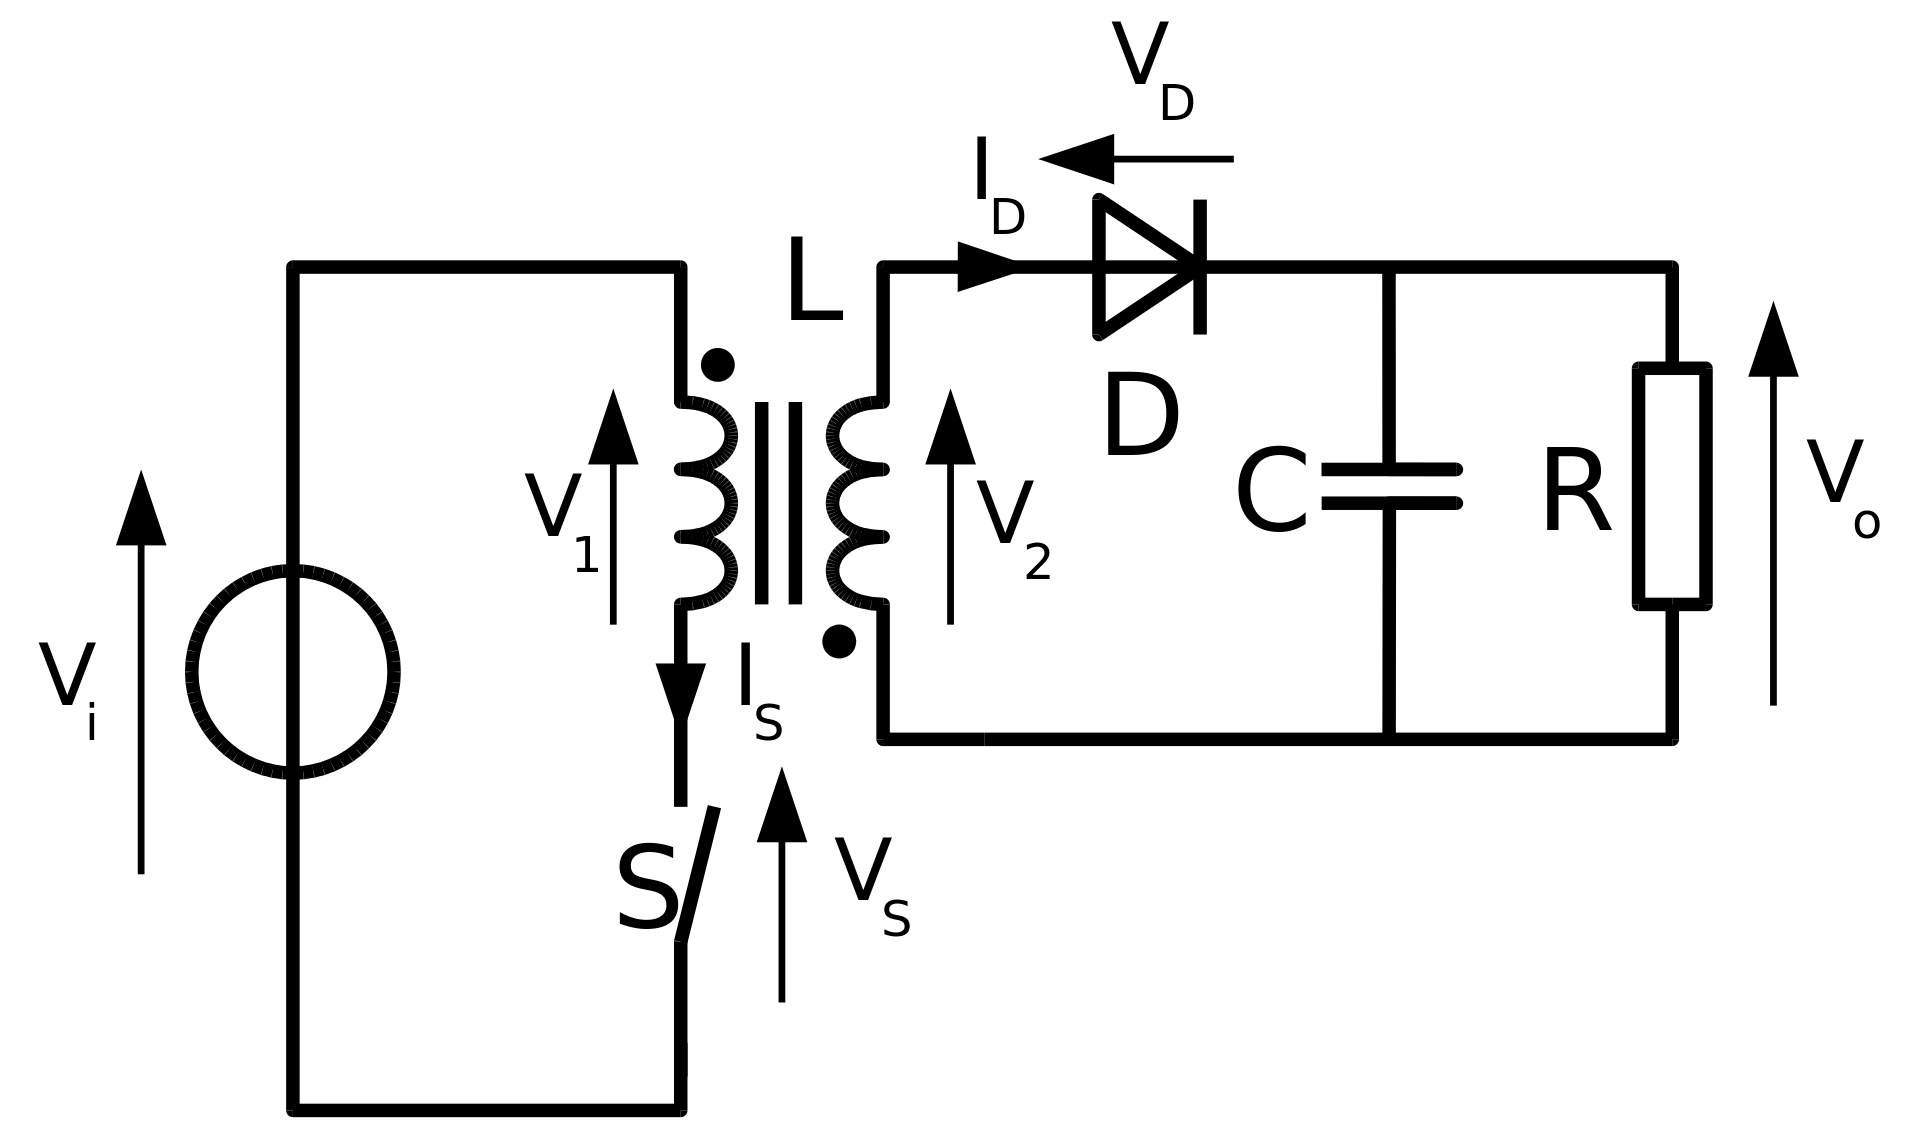
\includegraphics[width = 0.5\textwidth]{img/flyback.png}
        \caption{Flyback converter}
        \label{fig:flyback}
    \end{figure}

    Our alternative in choices were active clamp flyback converter and forward converter. The dominant advantages of active clamp topology are increased efficiency by applying ZVS and reduced switch voltage stress, which can also be achieved with snubbers in ordinary flyback converters. Although seemingly advantageous, we had to abandon the idea of active clamp flyback converter because all IC's we could find had startup voltages higher than the input voltage range of the project. This meant we had to use a digital controller, but it had to be quite precise to switch at the correct instant so that efficiency would be high and circuit would be linear. Our second alternative, forward converter, was disregarded because forward converter requires two inductors and two diodes. We preferred less components to deal with.
    \subsection{Parameter Selection}

    There are two main parameters in a flyback converter: the magnetizing inductance of the transformer and the turns ratio.

    \begin{itemize}

        \item DCM vs CCM selection:

        According to \cite{dcm}, peak MOSFET and diode currents are higher in DCM. Further, DCM losses are claimed to be higher than CCM losses. Combined with the fact that DCM means nonlinear operation, it may seem as if it is all negative. However, the same source provides the typical Bode plots of CCM and DCM, where we see that the control of DCM operation may be less tricky than CCM. Nonetheless, we selected an IC that can perform control. Thus, we chose CCM so that we could design our parameters in simpler linear relations.

        \begin{figure}[H]
            \centering
            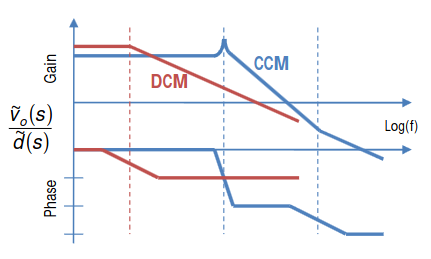
\includegraphics[scale=0.8]{img/bode.png}
            \caption{Bode plots in DCM and CCM}
            \label{fig:bode}
        \end{figure}

        \item Switch frequency $f_s$ selection:

        We decided to operate at 200 KHz because it is possible by both by analog and digital controllers. All other selections were made upon this selection.
        
        \item Turns ratio $N = \frac{N_2}{N_1}$ selection:

        Input voltage ranges between 12V and 18V while output voltage must remain constant. In the ideal lossless case the voltage relation of a flyback converter is given as:

        \begin{align*}
            V_o = \frac{N_2}{N_1}\frac{D}{1-D}
        \end{align*}

        Plot \ref{fig:DvsN} shows the variation of maximum and minimum required duty cycle with respect to different $N = \frac{N_2}{N_1}$.

        \begin{figure}[H]
            \centering
            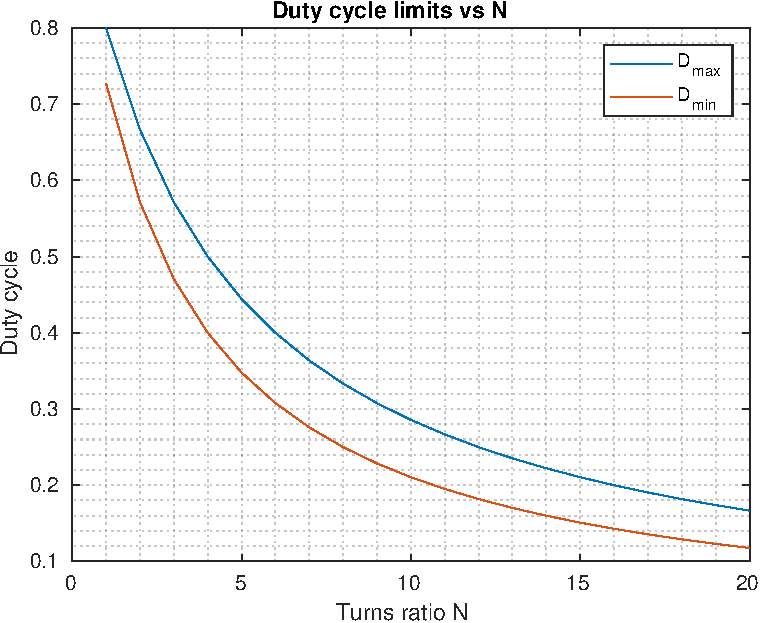
\includegraphics{img/DvsN.pdf}
            \caption{D vs N plot of Flyback converter}
            \label{fig:DvsN}
        \end{figure}
        
        Using this plot, we decided on out duty cycle range. 0.4-0.5 is a good nominal operating interval because it allows us to compensate for unprecedented increase and decrease requirements. Therefore, we set the turns ratio as $N = 4$.

        \item Magnetizing inductance $L_m$ selection:
        
        Next, we needed to determine the magnetizing inductance $L_m$. The key idea in choosing $L_m$ is to both ensure CCM is possible and to use as much of the flux bearing capabilities of the core as possible. We decided 40\% magnetizing current ripple is a reasonable value because it means we can continue to work in CCM even if load is much less than its rated value. 

        Similarly to the previous part, we have used MATLAB to create the plot of required magnetizing inductance for each input current average case. Then we made sure that the inductance value satisfies the maximum 40\% $i_M$ ripple constraint in all cases. To do so, we have used the characteristic plots of the flyback converter to derive the following relationship:

        \begin{align*}
            I_{LM, avg} = \frac{I_{in,avg}}{D}
        \end{align*}

        Then, assuming a predicted and not so absurd 88\% efficiency value, we determined the input current average for a number of input voltages. Finally, the given relation determines the $L_m$ value with respect to any desired current ripple and input current:

        \begin{align*}
            L_m = \frac{V_{in}D}{f_s\Delta I_{LM}}
        \end{align*}

        Figure \ref{fig:VinvsLm} illustrates the relationship between the input voltage and the required $L_m$ to ensure maximum 40\% magnetizing current ripple.

        \begin{figure}[H]
            \centering
            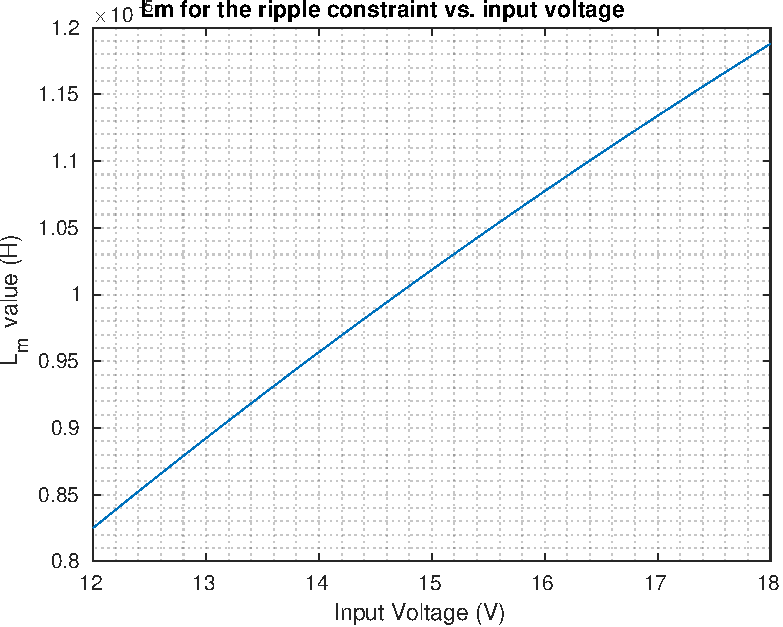
\includegraphics{img/VinvsLm.pdf}
            \caption{Required $L_m$ at each input voltage}
            \label{fig:VinvsLm}
        \end{figure}

        Referring to the Figure \ref{fig:VinvsLm} we decided to set $L_m = 12\mu$H. Note that this value overestimates $L_m$ than its ideal case. 
        
        Now we assure CCM operation and determine the output current limits for constant output voltage and varying input voltage. We continue with perfect efficiency in this calculation.

        At the DCM and CCM boundary, 
        \begin{align*}
            \Delta i_{LM} = 2 i_{LMavg}\\
            \frac{V_sDT_s}{L_m} = 2 i_{LMavg} =\frac{2i_{in,avg}}{D}\\
        \end{align*}

        \begin{table}[H]
        \centering
        \caption{DCM boundary output average currents at maximum and minimum input voltage}
        \begin{tabular}{|c|c|l}
        \cline{1-2}
        \textbf{Input Voltage (V)} & \textbf{DCM Boundary Current (mA)} &  \\ \cline{1-2}
        12                         & 156                                &  \\ \cline{1-2}
        18                         & 225                                &  \\ \cline{1-2}
        \end{tabular}
        \label{tab:DCM}
        \end{table}

        Referrring to Table \ref{tab:DCM}, we see that the least output current must be larger than 225 mA, which roughly corresponds to 25 \% load. Even in this case, we continue to operate at CCM.
    \end{itemize}

    Table \ref{tab:elec_sum} is a table summarizing the electrical parameters of our flyback converter.

    \begin{table}[H]
    \centering
    \caption{Electrical Parameters of the Converter}
    \begin{tabular}{|c|c|}
    \hline
    \textbf{Parameter} & \textbf{Value} \\ \hline
    DCM vs CCM         & CCM            \\ \hline
    $f_s$              & 200 KHz        \\ \hline
    N                  & 4              \\ \hline
    $L_m$              & $12\mu$H       \\ \hline
    \end{tabular}
    \label{tab:elec_sum}
    \end{table}


\newpage    
\section{Magnetic Design}

    After finalizing $L_m$ parameter, we then worked on magnetic design. A quick market research showed that many cores were not readily available on the market. Thus, we went on with a upcycled ferrite core. The reused ferrite core in hand is an E core made up of 3C94 material \cite{core}.
    
    The concerns in magnetic design are whether or not the core gets saturated, if and how much air gap must be present and whether or not there is enough room to wind the wires around the legs of the core.
    \subsection{Core Design}

    Figure \ref{fig:photo of core} is a photograph of our E core. All decisions are made for this core. There are two main parameters in core design; namely, air gap length and turn number.

    \begin{figure}[H]
        \centering
        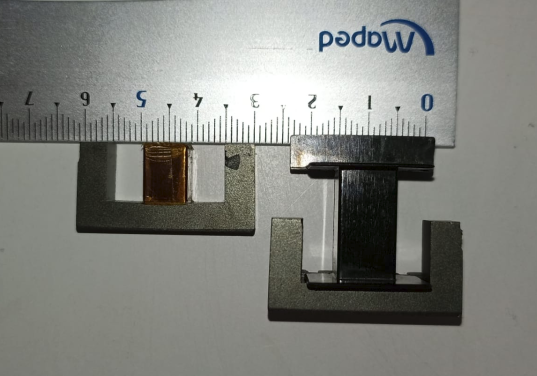
\includegraphics[width=0.5\textwidth]{img/core.png}
        \caption{Our E core}
        \label{fig:photo of core}
    \end{figure}

    Firstly, an air gap is necessary for flyback converters because flyback converter stores energy in the core during on time and releases the energy to the load during off time. Therefore, air gap is used to enhance the energy storing capability of the core.

    \begin{itemize}
        \item Gap length and primary side winding turn number:

        Up to this point, we only had the decision of $L_m = 12\mu$ H at hand and the inductance relation:

        \begin{align*}
            L = \frac{N_p^2}{R}
        \end{align*}

        Reluctance is a function of air gap length so inductance is a function of both decision parameters. As an easy way of choosing both parameters at once, we decided to plot the variation of one parameter with respect to the other for the given inductance value. Since the permeability of air is much smaller than ferrite material, reluctance of the core with the gap almost equals the reluctance of the air gap. Therefore, we assumed core reluctance is zero without the air gap to have a sense of air gap and turn number. Figure \ref{fig:airgapvsturns} is the plot we obtained.

        \begin{figure}[H]
            \centering
            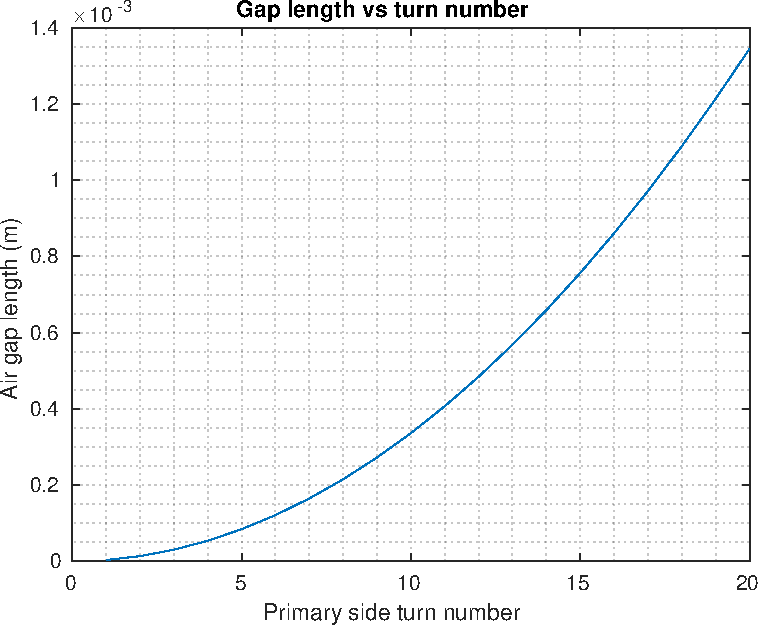
\includegraphics{img/airgapvsturns.pdf}
            \caption{Air gap length and primary side turns for $L_m = 12\mu$H}
            \label{fig:airgapvsturns}
        \end{figure}

        After some iterations, we set primary side turn number to 9 so that air gap length is approximately 0.27mm. For reference, thickness of A4 paper is almost 0.1 mm. Note that almost 3 papers thick air gap verifies our approximation for the equivalent reluctance. Indeed, the reluctance of the air gap is  6750000 $\frac{Aturns}{Wb}$.
        
        \item Core magnetic flux density:

        One of the most important criteria in core design is ensuring the core stays linear, at least however much real life permits. To check this, maximum possible magnetizing current peak should not disrupt core linearity. In other words, such a flux should not lead to saturation.

        We have used the approximate reluctance value to sweep across primary peak currents to obtain the operating level flux densities. 

        \begin{align*}
            I_{pri,peak} = I_{LMavg} + I_{LMavg}\frac{ripple \: ratio}{2}
        \end{align*}

        The outer legs of the E core are slightly smaller in area than the middle leg. Therefore, magnetic flux densities are different at these two types of legs. We see both densities in figure \ref{fig:B}.

        \begin{figure}[H]
            \centering
            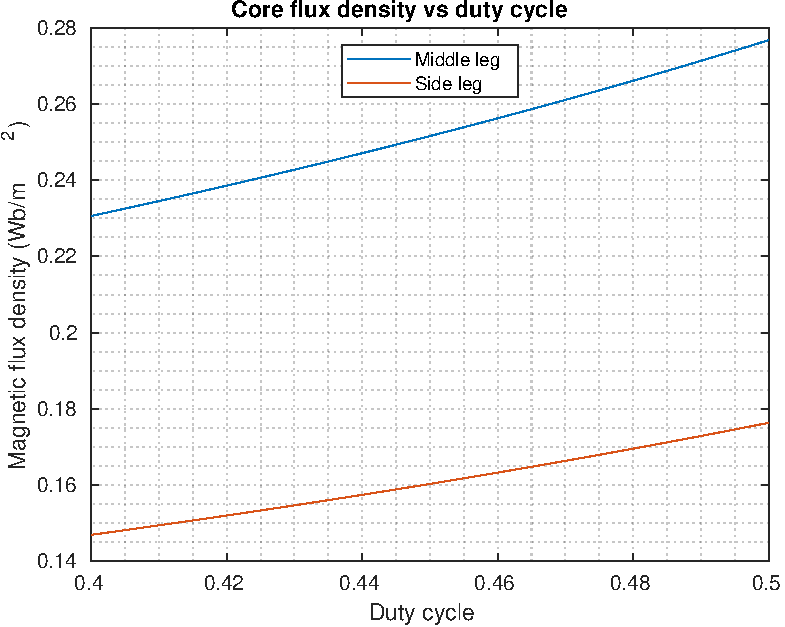
\includegraphics{img/B.pdf}
            \caption{B field density vs duty cycle}
            \label{fig:B}
        \end{figure}

        The material saturates at around 300 mT \cite{core} so we are within the limits and the converter remains linear.
    \end{itemize}
    
        \begin{table}[H]
        \centering
        \caption{Core design parameters}
        \begin{tabular}{|c|c|}
        \hline
        \textbf{Parameter}         & \textbf{Value} \\ \hline
        Primary side turn number   & 9              \\ \hline
        Secondary side turn number & 36             \\ \hline
        Air gap length             & 0.27mm         \\ \hline
        B field                    & 140 mT - 280 mT \\ \hline
        \end{tabular}
        \label{tab:core}
        \end{table}

    
    \subsection{Winding Design}
    For the actual wires of the flyback transformer we considered two alternatives. The first analysis is done with standard single strand copper wires. First consideration on this is the skin depth since the switching frequency is selected as 200 kHz and related AC losses are affected by skin depth a lot. For the selected $F_{sw}$ the skin depth results in,

    \begin{equation*}
        \delta = \sqrt{\frac{\rho}{\pi F_{sw} \mu_0 }} = 1.4587\cdot 10^{-4}m
    \end{equation*}

    Later, maximum allowable strand cross-section is yields,
    
    \begin{equation*}
        \textrm{Strand Area} = \pi \delta ^2  = 0.0668 mm^2 
    \end{equation*}

    \subsubsection{Solid Copper Variant}

    
    This is around 29 AWG. Current rating of this wire gauge is 0.182 amperes however we can define a risk factor to push the copper a little more to utilize the core more effectively. In another words, with a risk factor of 2 double the amount of current will pass through the wire.

    The RMS of the input current is calculated as 4.55 amperes.
    Number of primary strands is, this RMS current divided into each strand. The result is we would need 33.3 parallel strands.

    \begin{center}
    ------------------------------------------------ \\
    A side note on this is that the input current is highly discontinuous at the switching frequency. It does not have a ripple over a fixed current hence by the frequency decomposition, the component at the switching frequency is quite large. \\
    -------------------------------------------------- \\
    \end{center}
    %\raggedright
    
    For the secondary side, same analysis can be made. Again using the RMS value of the current over the transformer. This results in 7.33 parallel strands.

    Primary wire count is number of parallel strands multiplied with the turn number,

    \begin{equation*}
        \textrm{Primary Wire Area} = N_{pri} \cdot primary\_parallel = 1.9391\cdot 10^{-5}
    \end{equation*}

    For the secondary

    \begin{equation*}
        \textrm{Secondary Wire Area} = N_{pri} \cdot turns\_ratio \cdot secondary\_parallel = 1.7064\cdot 10^{-5}
    \end{equation*}

    Numbers seem high however this consist of both parallel strands and the full wire length and it will be used to calculate the fill factor.
    \begin{equation*}
        \textrm{Fill Factor} = \textrm{Total Wire Area} / \textrm{Total Window Area} =   31.87 \%
    \end{equation*}

    \subsubsection{Litz Variant}

    Although the parallel wires are effectively acting as litz wires, a design with the actual litz wires are made, The design is given below and the total copper and fill factor are similar. This second design is expected to be better since the proximity and skin effect related losses will be less.

    \begin{table}[H]
        \centering
        \begin{tabular}{|c|c|l}
        \cline{1-2}
        \textbf{Turn Numbers} & \textbf{Wire Diameter and \# of Parallel} &  \\ \cline{1-2}
        9                         & 0.9 mm $\cross$ 2                                &  \\ \cline{1-2}
        36                         & 0.9 mm $\cross$ 1                                  &  \\ \cline{1-2}
        \end{tabular}
        \caption{Transformer Winding Design with Litz Wire}
        \label{tab:DCM}
    \end{table}

    The fill factor of the design with litz wire is calculated as $30\%$

    This fill factors are both within the reasonable limits. The fill factors of 30 percent can be easily wound. The expected fill factor is actually will be smaller since the litz wire have around 1.28 packing factor which means that it has 0.22 percent empty spaces inside. On the hand created litz case, this is expected to be lower.

    \begin{figure}[H]
        \centering
        \sbox0{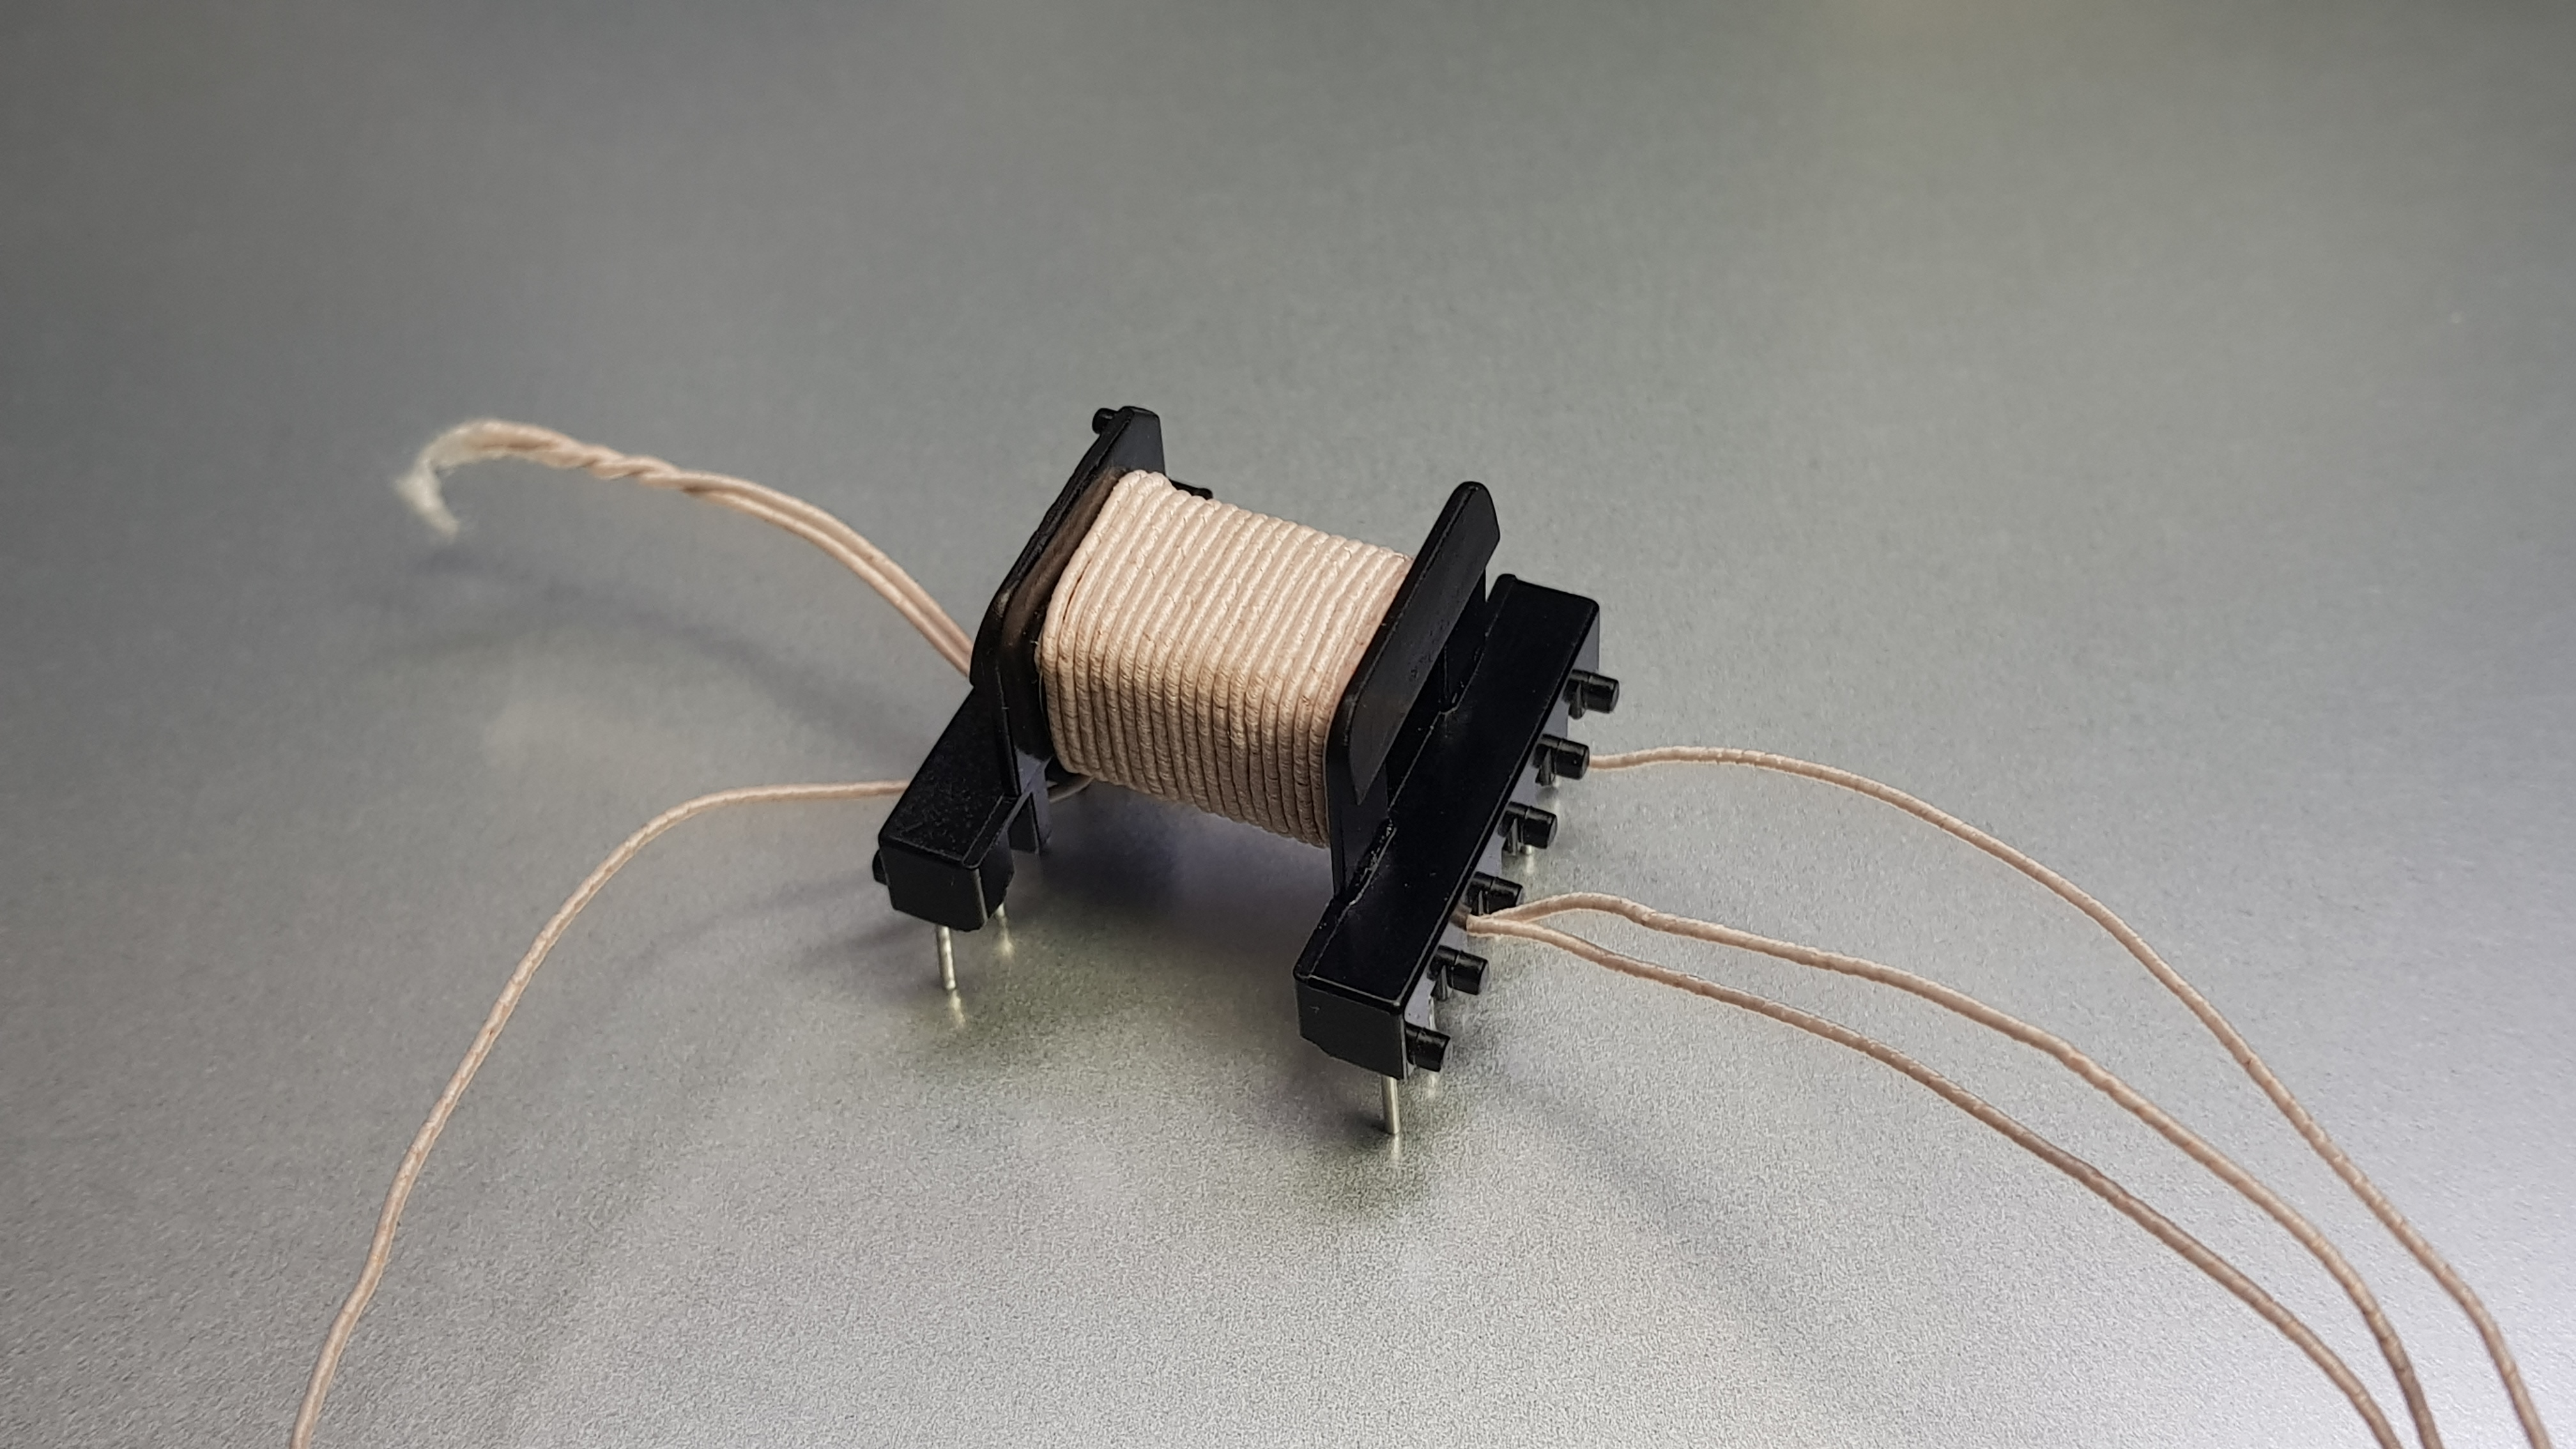
\includegraphics{img/tr_1.jpg}}%
        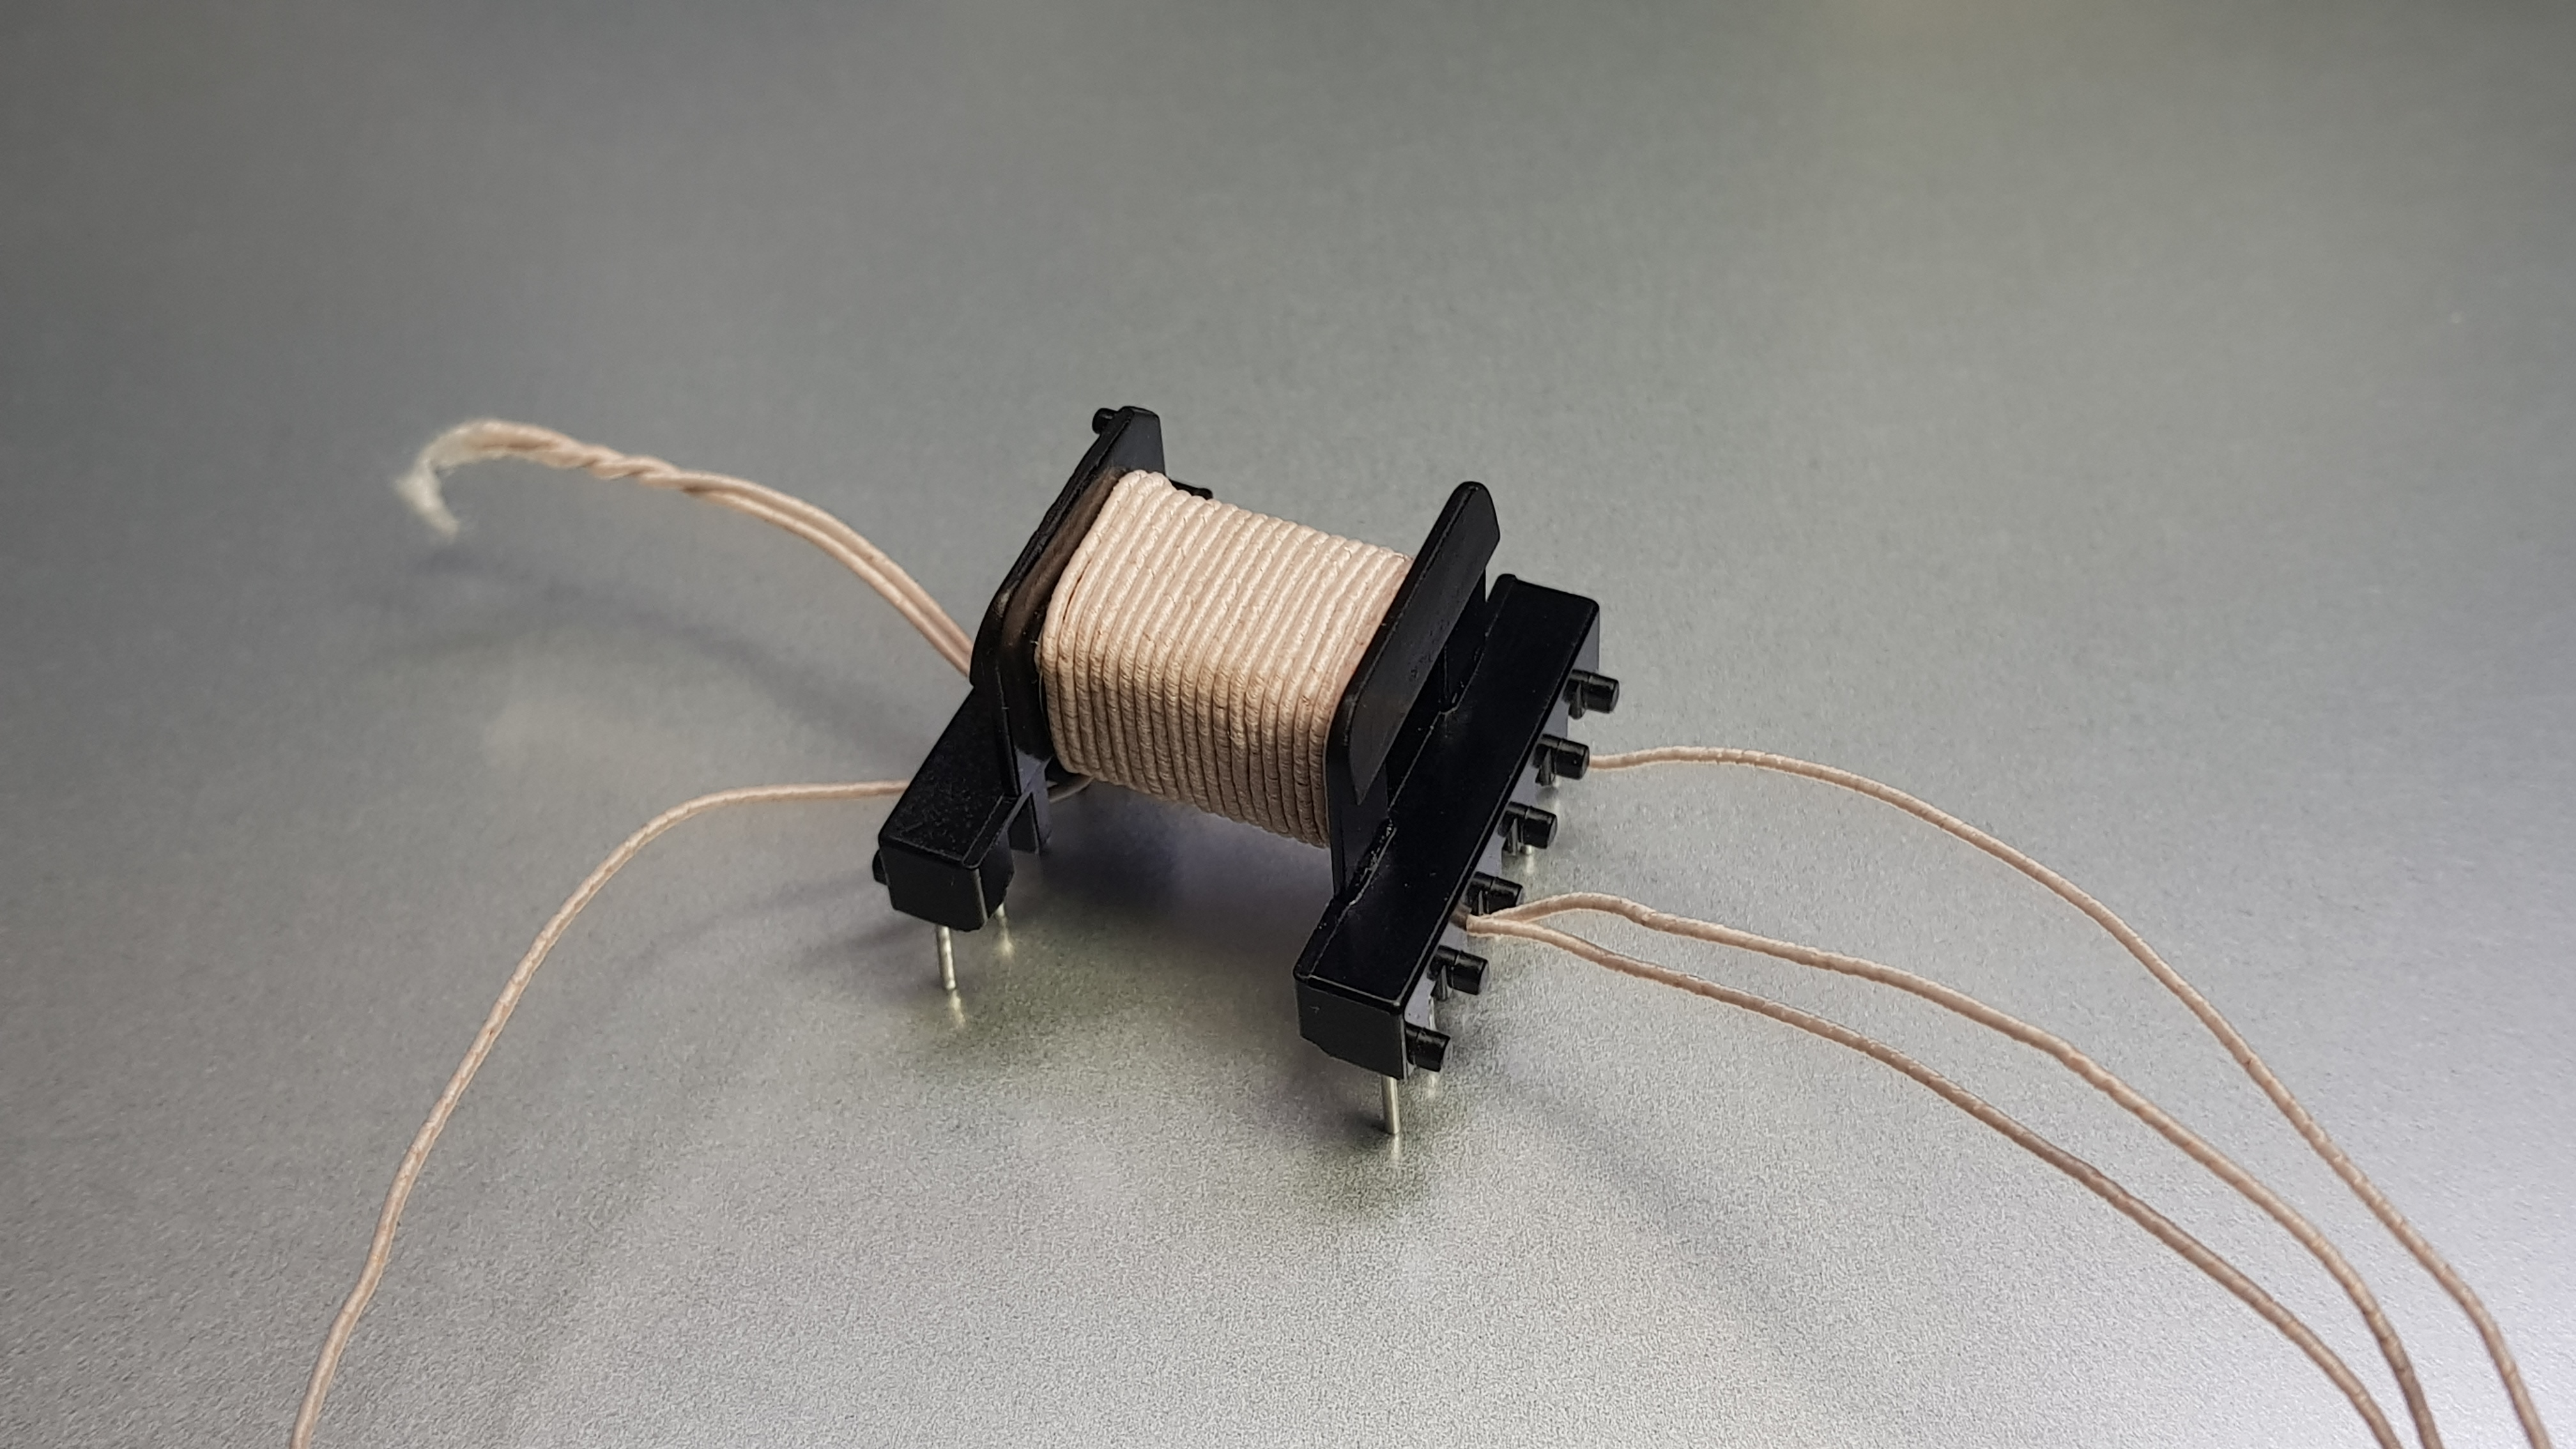
\includegraphics[clip,trim={.15\wd0} {.2\ht0} {.15\wd0} {.22\ht0},scale = 0.12]{img/tr_1.jpg}
        \caption{Photograph of the first version with Litz wire. (Fill factor 30\%)}
        \label{fig:tr_1}
    \end{figure}

    Later it is deduced that the core had plenty empty spaces inside.This space can be filled with copper to reduce the copper loss for the transformer, however the leakage inductance will get higher due to the windings move away from the center of the core. A new version for the litz is wound. This time the fill factor of the E cores with the litz cable is expected to be around 80\% if wound tightly. The primary side wound with a cable that has double the previous wire diameter without paralleling and secondary side kept at the same cable dimensions with 2 parallels.


    \begin{table}[H]
        \centering
        \begin{tabular}{|c|c|l}
        \cline{1-2}
        \textbf{Turn Numbers} & \textbf{Wire Diameter and \# of Parallel} &  \\ \cline{1-2}
        9                         & 1.8 mm $\cross$ 1                                &  \\ \cline{1-2}
        36                         & 0.9 mm $\cross$ 2                                  &  \\ \cline{1-2}
        \end{tabular}
        \caption{Transformer Winding Design with Litz Wire}
        \label{tab:DCM}
    \end{table}

    The fill factor of the design with litz wire is calculated as $60\%$

    \begin{figure}[H]
        \centering
        \sbox0{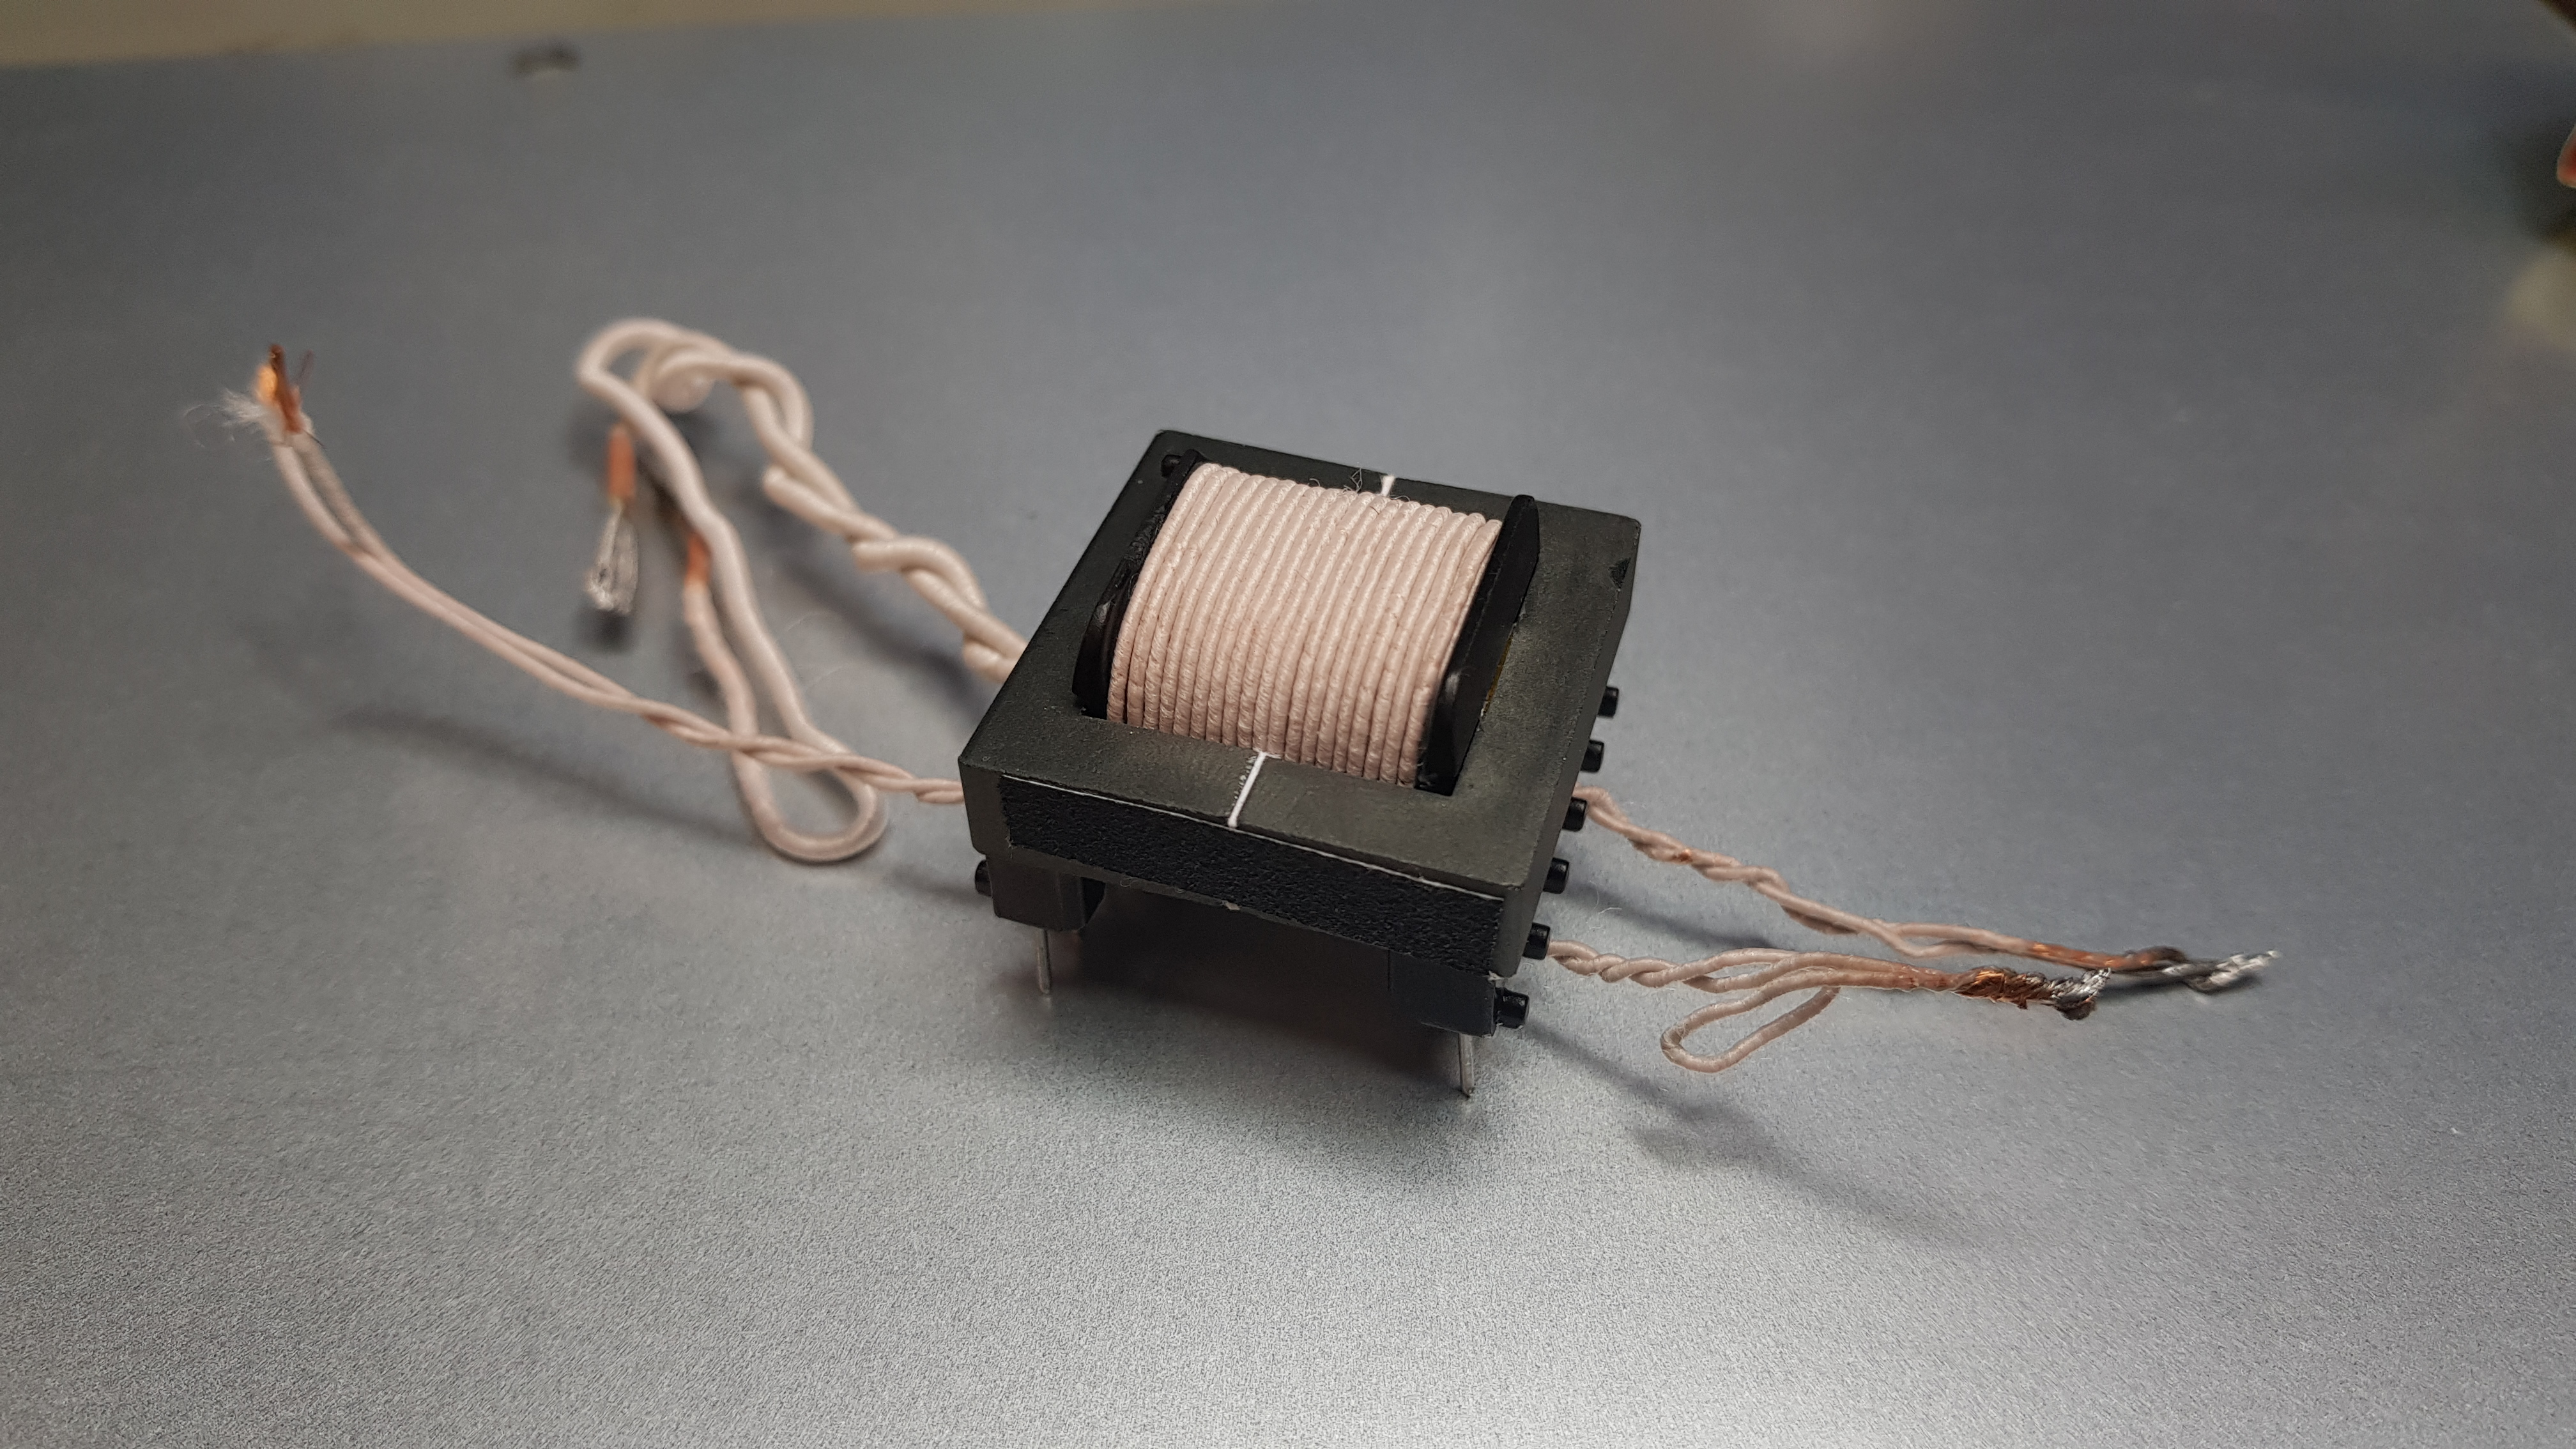
\includegraphics{img/tr_2.jpg}}%
        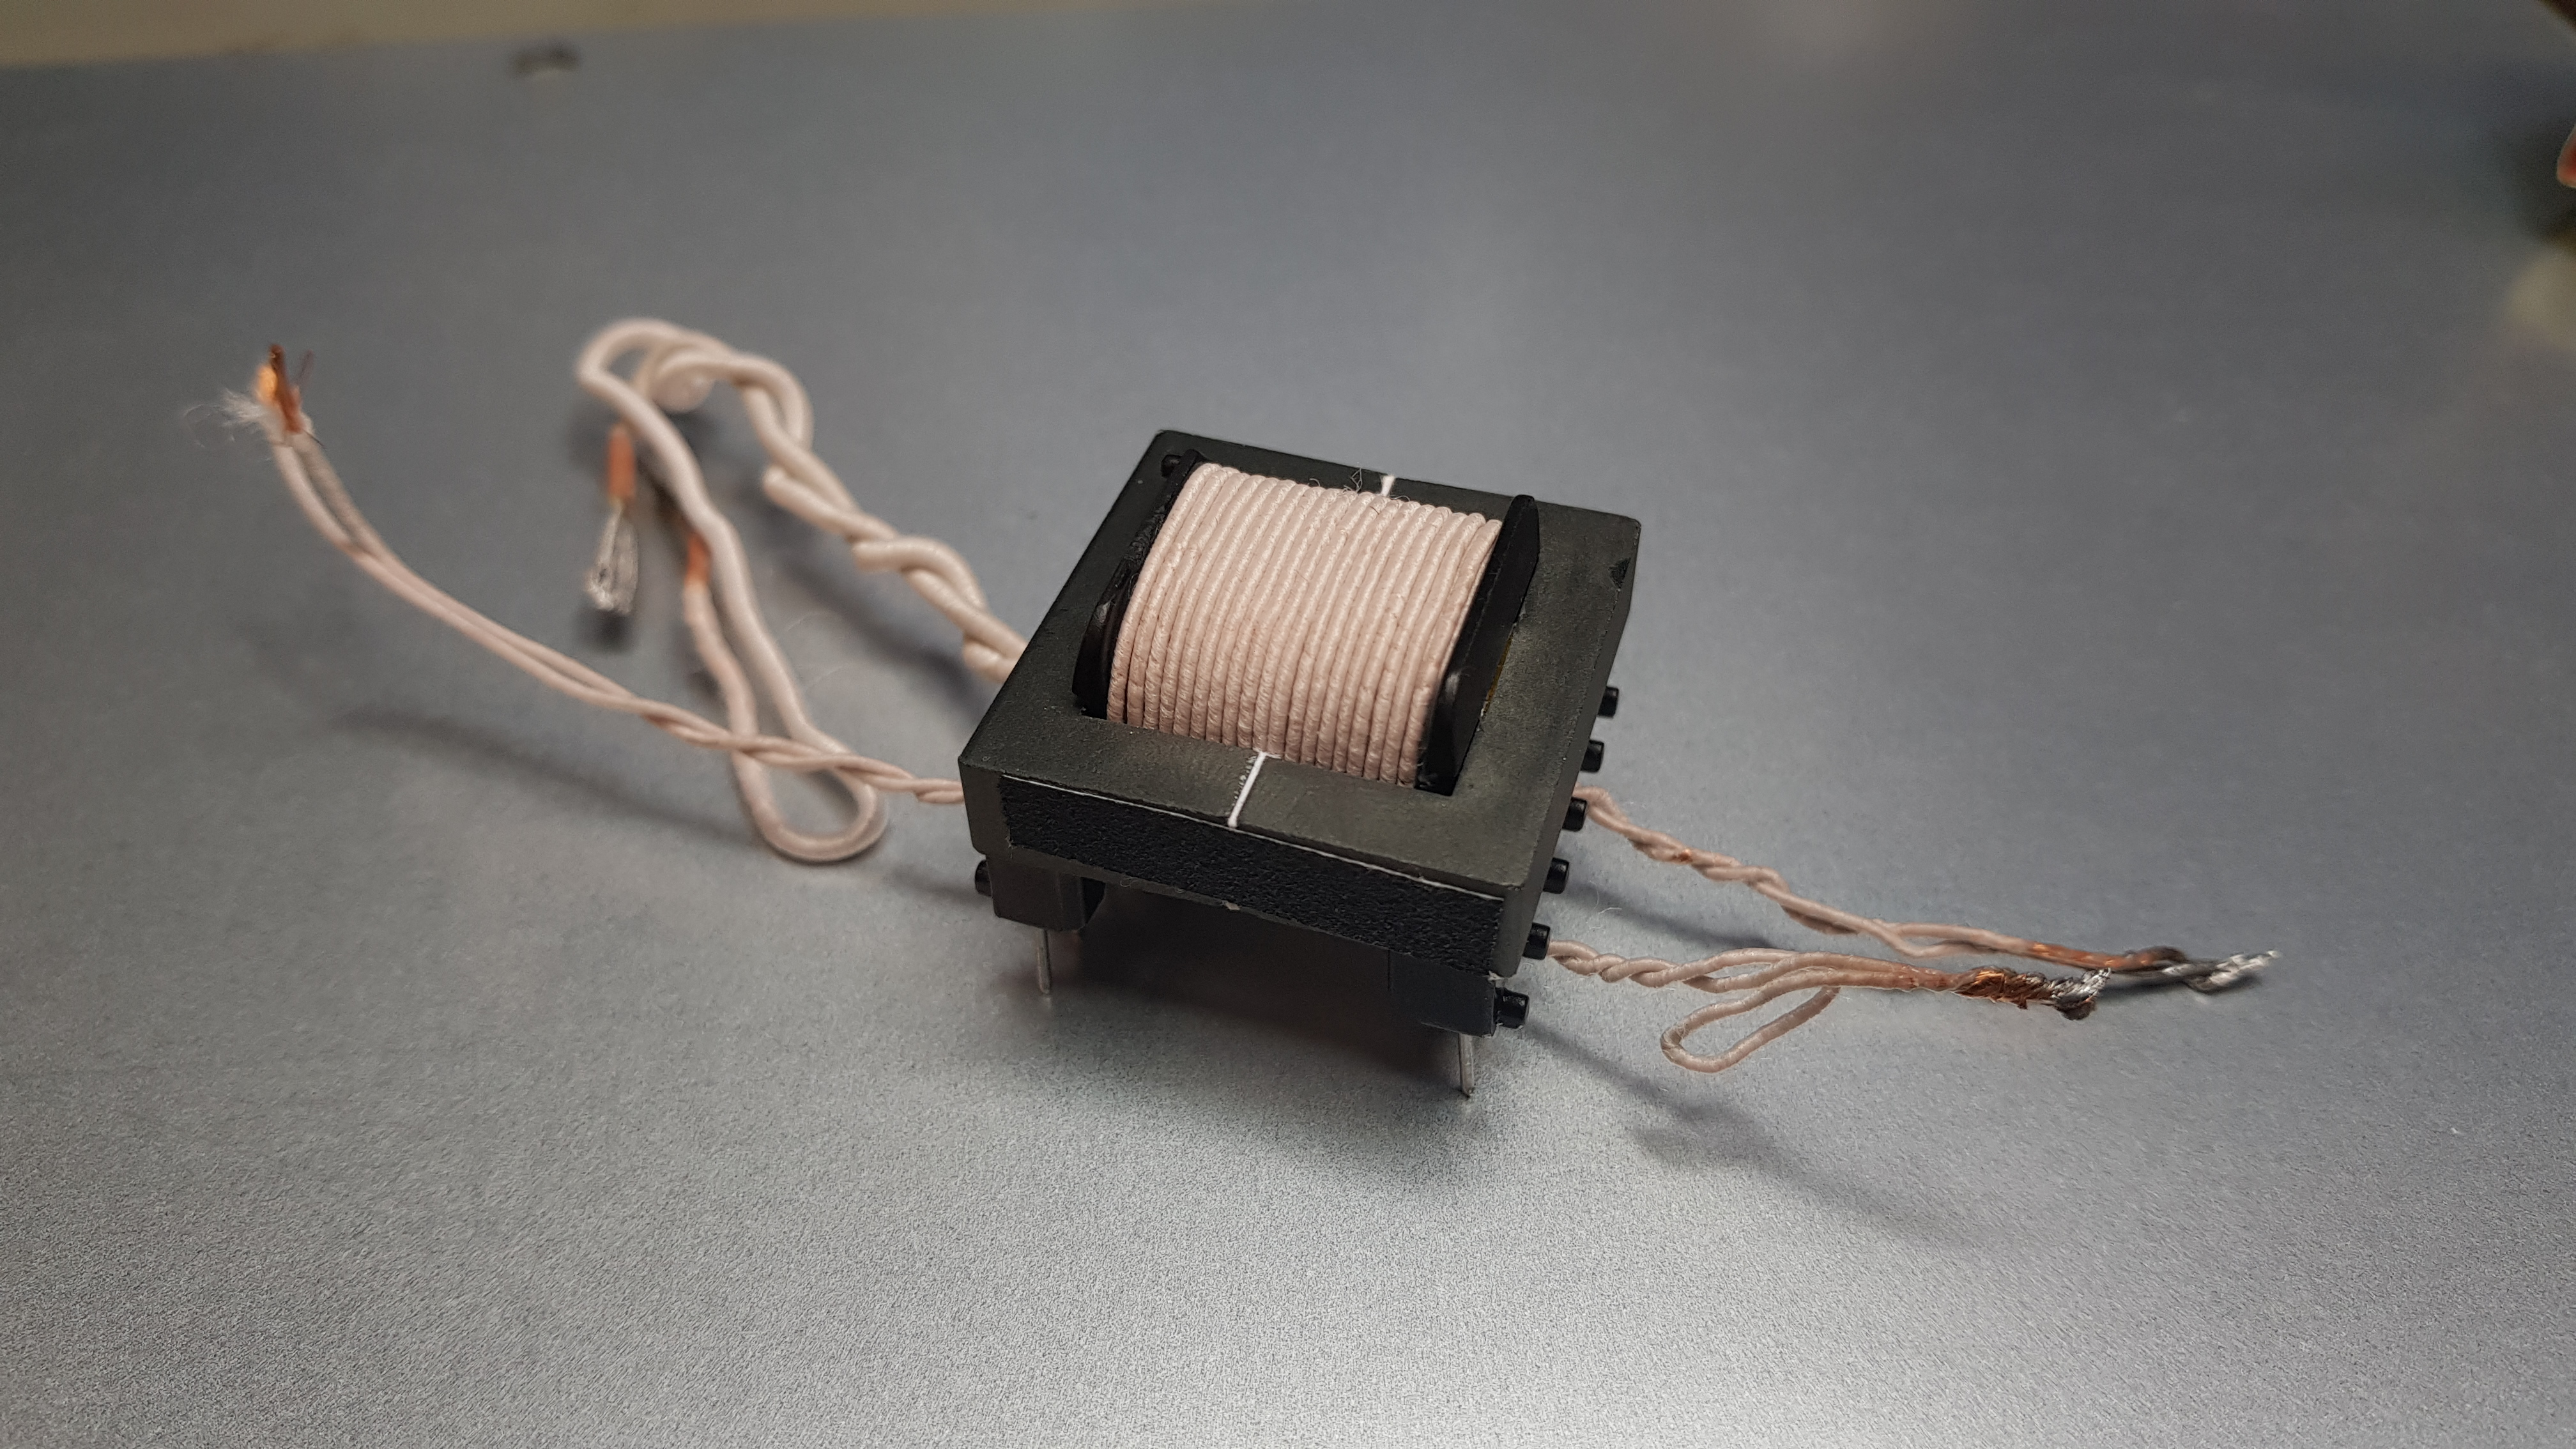
\includegraphics[clip,trim={.15\wd0} {.18\ht0} {.15\wd0} {.2\ht0},scale = 0.12]{img/tr_2.jpg}
        \caption{Photograph of the second version with Litz wire. (Fill factor 60\%)}
        \label{fig:tr_2}
    \end{figure}

    For the winding configuration, the layers are arranged such that first the half of the secondary is wound, then the primary is placed covered with the rest of the secondary. The sandwich pattern helps with reducing the leakage inductance.

    \subsubsection{Measurements of the Core}

    The core is then measured, $L_{pri} = 12.42 \mu H$, $L_{sec} = 192.8 \mu H$ \\

    
    A quick check for the turns ratio which should be 4, 

    \begin{equation*}
        \frac{N_{sec}}{N_{pri}} = \sqrt{\frac{192.8\mu H}{12.42 \mu H}} = 3.94 \simeq 4
    \end{equation*}

    For the leakage inductances measured from primary and secondary,\\
    $L_{leak\_pri} = 0.32\mu H$, $L_{leak\_sec} = 4.97 \mu H$ \\

    Leakage inductance came out to be $2.5\%$.

    

    

    \subsection{Losses}   
    \subsubsection{Copper Loss}
    For the copper loss we need to calculate the wire primary and secondary, total wire lengths.

    The primary wire length calculated is 0.3341 meters. The secondary counterpart is 2.6964 meters.

    The resistance is calculated as,

    \begin{equation*}
        \textrm{R\_pri} = \frac{\rho l_{pri}}{A\cdot N_{parallel}} = 0.0056 \Omega
    \end{equation*}    

    \begin{equation*}
        \textrm{R\_sec} = \frac{\rho l_{sec}}{A\cdot N_{parallel}} = 0.0911 \Omega
    \end{equation*}    

    Power is then $P = i\cdot R^2$ with the RMS currents.

    The total copper loss is, for primary 0.3242 W and for secondary 0.2083 W.

    Total is calculated at the highest currents hence the performance will be better.

    \subsubsection{Core Loss}

    The core loss is calculated from the power loss density and the peak magnetic flux density curves at fixed frequency given by the manufacturer on the datasheet of the related core.

    These are empirical values and the our selected data is from 200 kHz line.

    The datapoints from the datasheet is digitized on matlab and a polynomial equation is fitted. 

    The magnetic flux density is different on the side legs of the E core than the center leg hence two volumes are calculated separately. 

    The total loss is calculated from the $\Delta B $ but the data is for AC magnetic flux variation hence $\Delta B $ given is expected as the right approach for more accurate calculation. A safety factor of 2 is given for margins of errors. The total core loss for highest operation is found as 1.22 W.



    
\newpage
\section{Controller Design}
    UC3843 allows for cascade peak current and voltage control. Both functionalities of the IC are used. The following circuit diagram \ref{fig:datasheet_circuit} is taken from the datasheet of UC3843 \cite{ic} and demonstartes the recommended operation of the PWM controller. 
    
    \begin{figure}[H]
        \centering
        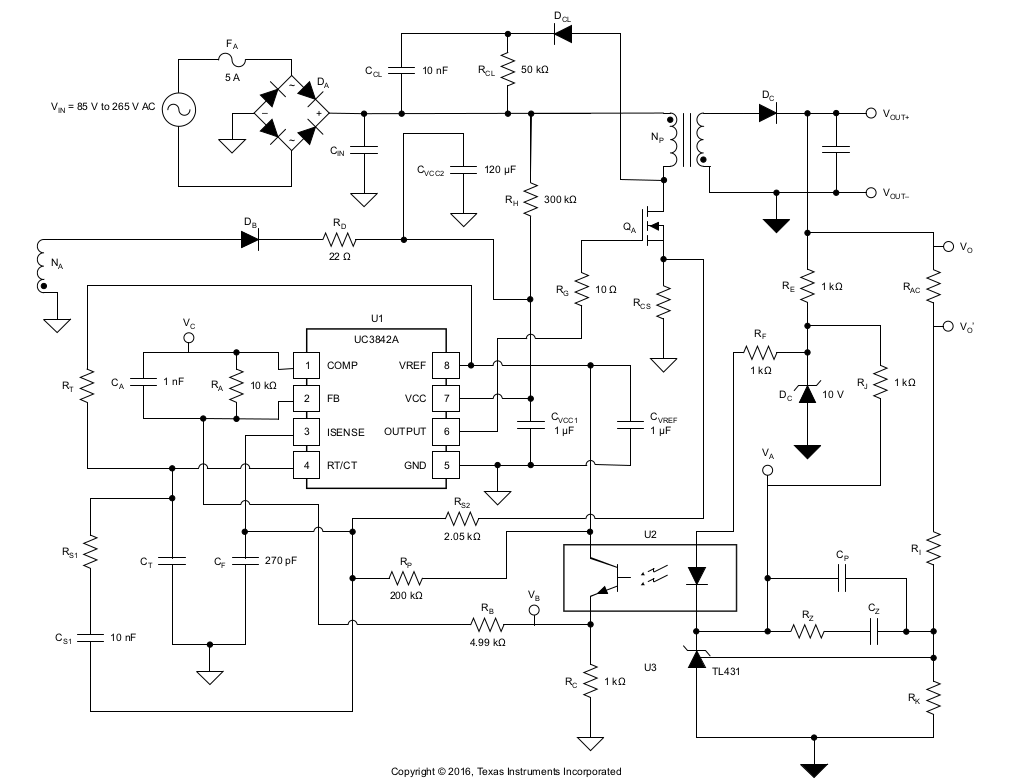
\includegraphics[width = \textwidth]{img/circuit_datasheet.png}
        \caption{Circuit diagram demonstrating the recommended application of UC3843A \cite{ic}}
        \label{fig:datasheet_circuit}
    \end{figure}
    
    We have implemented the recommended control circuit. Since our input is already DC we do not have the rectifier section as well as the auxiliary winding. In addition, we have decided to discard the pole placement capacitor $C_P$ for the optocoupler network because we have achieved a satisfactory performance without its tuning. The circuit schematic with the values we have used for the components are given in Figure \ref{fig:circuit_schematic}.

    \begin{figure}[H]
        \centering
        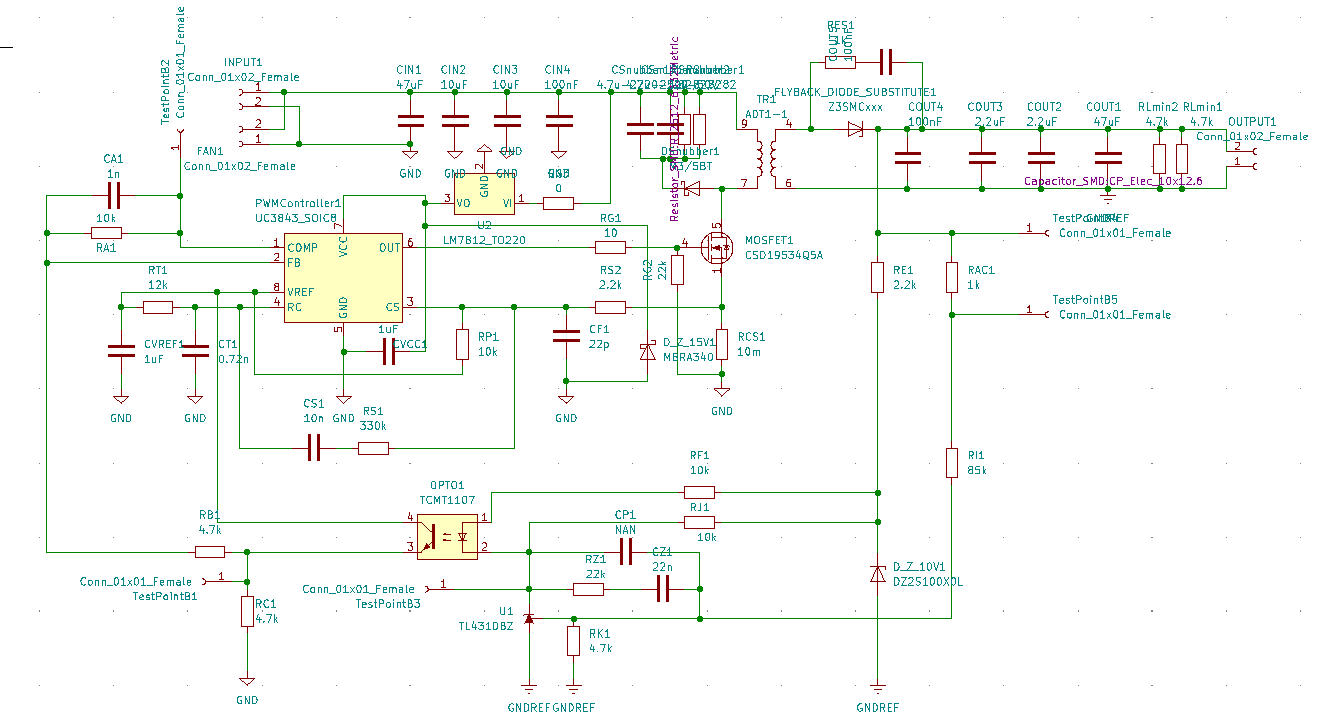
\includegraphics[width= \textwidth]{img/circuit_schematic.png}
        \caption{Circuit schematic with R and C values used in the circuit. Input and output capacitance may differ.}
        \label{fig:circuit_schematic}
    \end{figure}
    
    While components like $R_z$, $C_z$, $R_A$, $C_A$, $R_B$ are tuned by trial and error, some components entailed detailed calculations. To begin with, $R_K$ and $R_L$ are selected to set 2.5V at TL431 reference when output is exactly 48V. Pull up resistor for the current sense leg $R_P$ is set as 10.67 $k\Omega$ to set the operating range of the current sense leg to in between 0.6 and 0.8V approximately with 10$m\Omega$ current sense resistor. This value for the pull up resistor was determined by simulations. $R_T$ and $C_T$ are determined according to the formula $f_s = 1.72/(R_TC_T)$. 


    \begin{table}[H]
    \centering
        \begin{tabular}{cc}
        \textbf{Component}   & \textbf{Value ($\Omega$ for resistors, F for capacitors)} \\
        $R_A, R_F, R_J, R_P$ & 10k                                                       \\
        $R_B, R_C, R_K$      & 4.7k                                                      \\
        $R_E, R_S$           & 2.2k                                                      \\
        $R_{G2}, R_Z$        & 22k                                                       \\
        $C_A$                & 1n                                                        \\
        $C_F$                & 220p                                                      \\
        $C_S$                & 10n                                                       \\
        $C_T$                & 0.72n                                                     \\
        $C_Z$                & 22n                                                       \\
        $R_{AC}, R_{ES}$     & 1k                                                        \\
        $R_{CS1}$            & 10m                                                       \\
        $R_G$                & 10                                                        \\
        $R_I$                & 85k                                                       \\
        $R_S$                & 330k                                                      \\
        $R_T$                & 12k                                                      
        \end{tabular}
    \caption{Values used in the control circuit}
    \end{table}

\section{Computer Simulations \& Analysis}

    \subsection{Ideal Simulations}
    After determining a value for $L_m$, ideal simulations are done in LTspice. Ideal Flyback converter circuit constructed for the simulation is given in Figure \ref{fig:ideal_sim_circuit}. The model includes an ideal diode, an almost ideal switch, an ideal transformer model with magnetizing inductance, and an output capacitance whose value is calculated to make output peak-to-peak voltage ripple equal to $2\%$. The components named with "spice magic" are only included to increase simulation speed.  \\
    
    \begin{figure}[H]
        \centering
        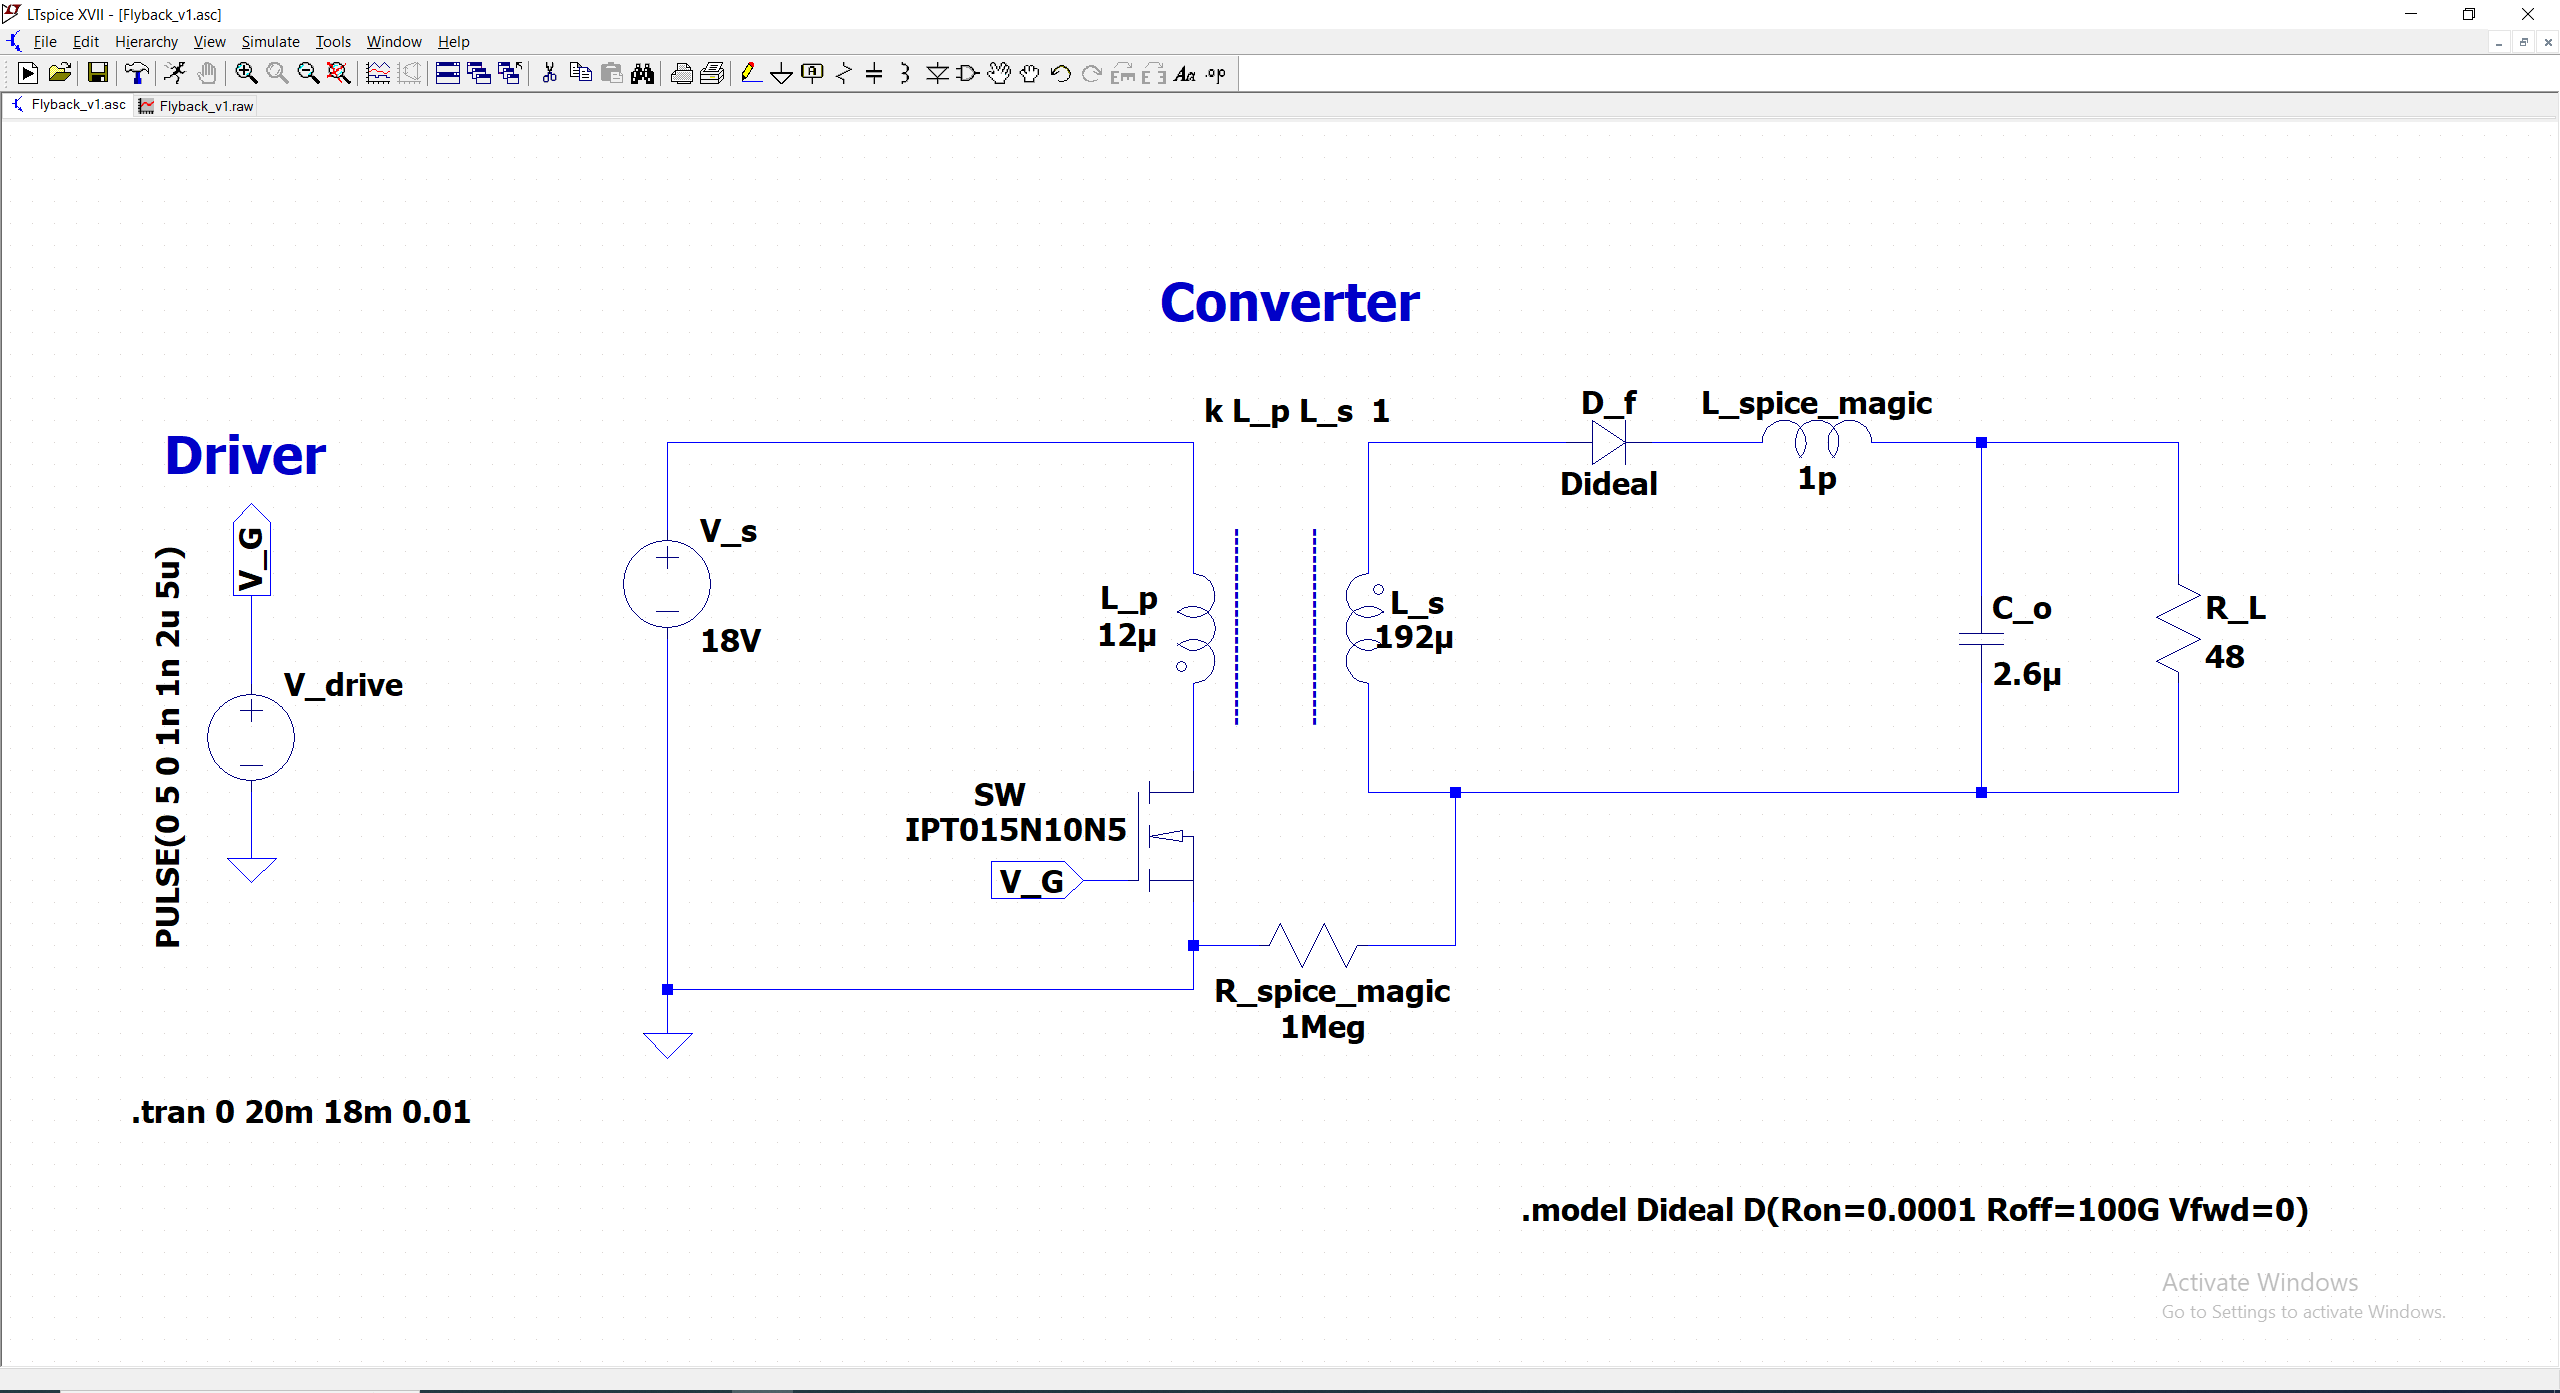
\includegraphics[scale=0.3]{img/Spice_Sim/Ideal/ideal_simulation_circuit.PNG}
        \caption{Simulated LTspice circuit schematic (ideal case)}
        \label{fig:ideal_sim_circuit}
    \end{figure}

    The design choices were made so that the magnetizing current ripple is at least $40\%$. Primary and secondary current waveforms are given in Figures \ref{fig:ideal_Lm_ripples_12V} and \ref{fig:ideal_Lm_ripples_18V} for $12V$ and $18V$ input voltages, respectively. As one can see, we have desired current ripple which is consistent with our design. \\

    \begin{figure}[H]
        \centering
        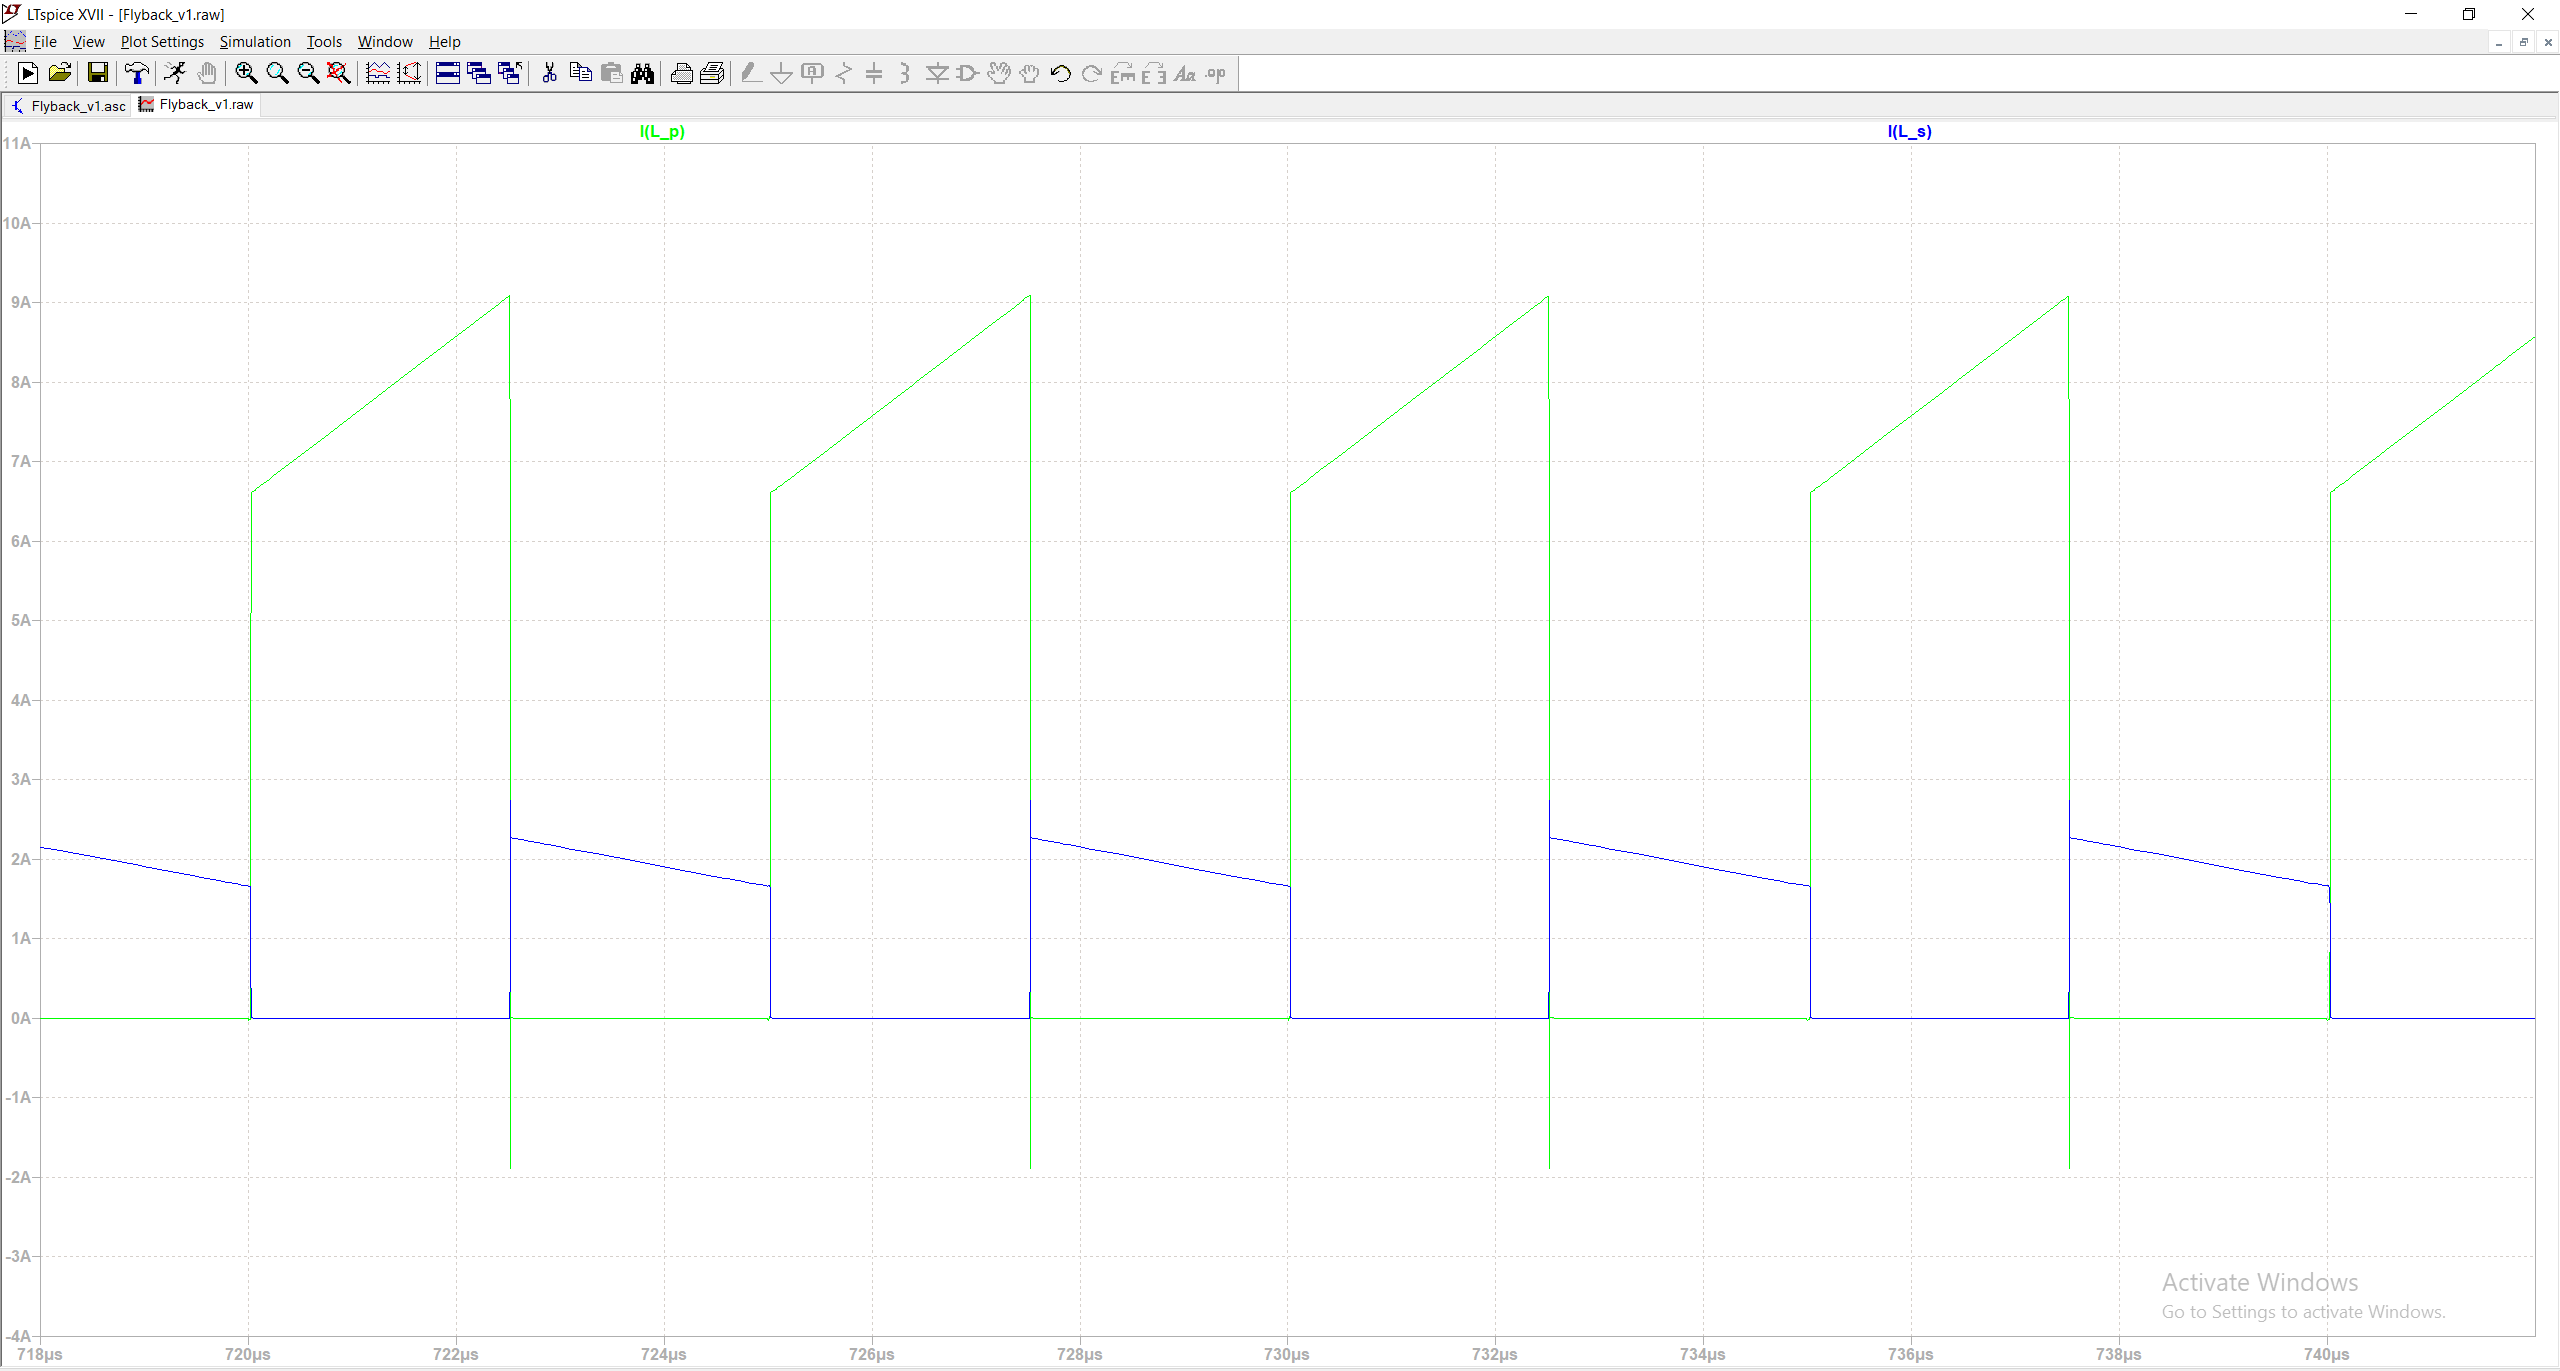
\includegraphics[scale=0.3]{img/Spice_Sim/Ideal/ideal_Lm_ripples_12V.PNG}
        \caption{Primary and secondary current waveforms for 12V input voltage}
        \label{fig:ideal_Lm_ripples_12V}
    \end{figure}

    \begin{figure}[H]
        \centering
        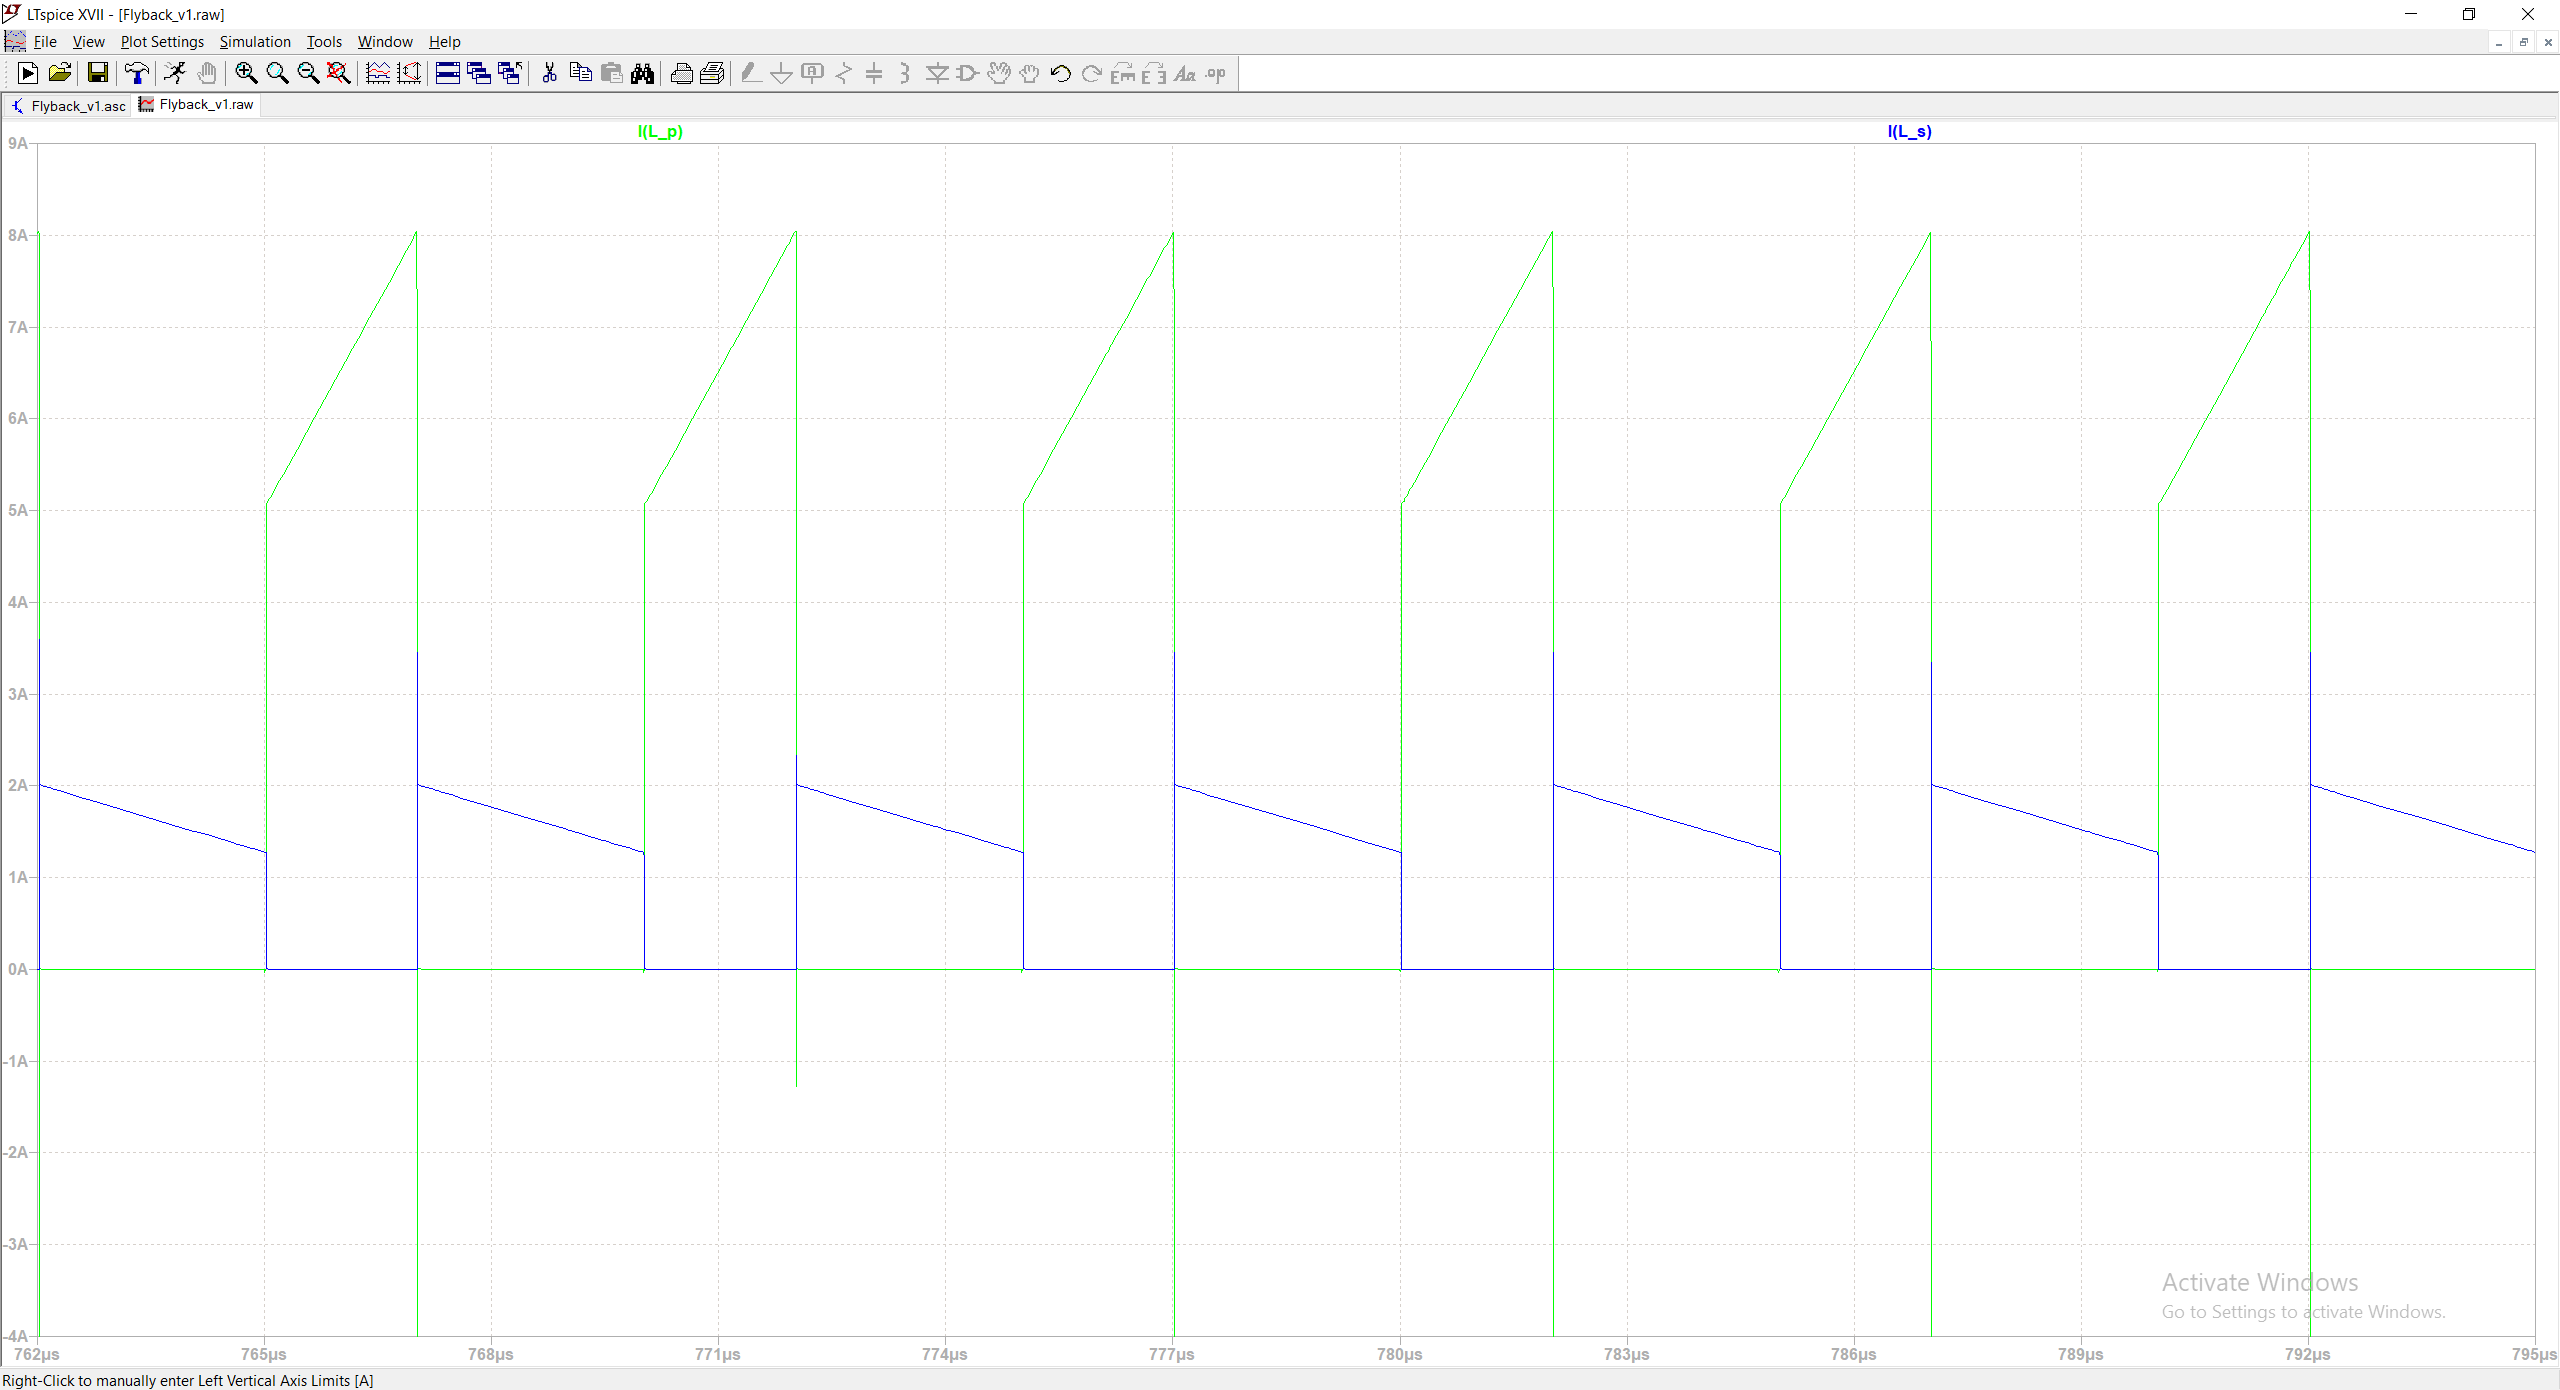
\includegraphics[scale=0.3]{img/Spice_Sim/Ideal/ideal_Lm_ripples_18V.PNG}
        \caption{Primary and secondary current waveforms for 18V input voltage}
        \label{fig:ideal_Lm_ripples_18V}
    \end{figure}

    We also observed the voltage stresses on the diode and on the switch in the simulation. The expected switch voltage during the off times are calculated as $V_{SW} = V_s + V_o\frac{N1}{N2} = 30V$, which is calculated for 18V input voltage (worst case). Also, the diode voltage is calculated as $V_D = V_s\frac{N2}{N1}+V_o = 120V$ during on times of the switch, again for the worst case. One can see from Figure \ref{fig:ideal_V_stress} that the simulation result is consistent with the theoretical one. \\

    \begin{figure}[H]
        \centering
        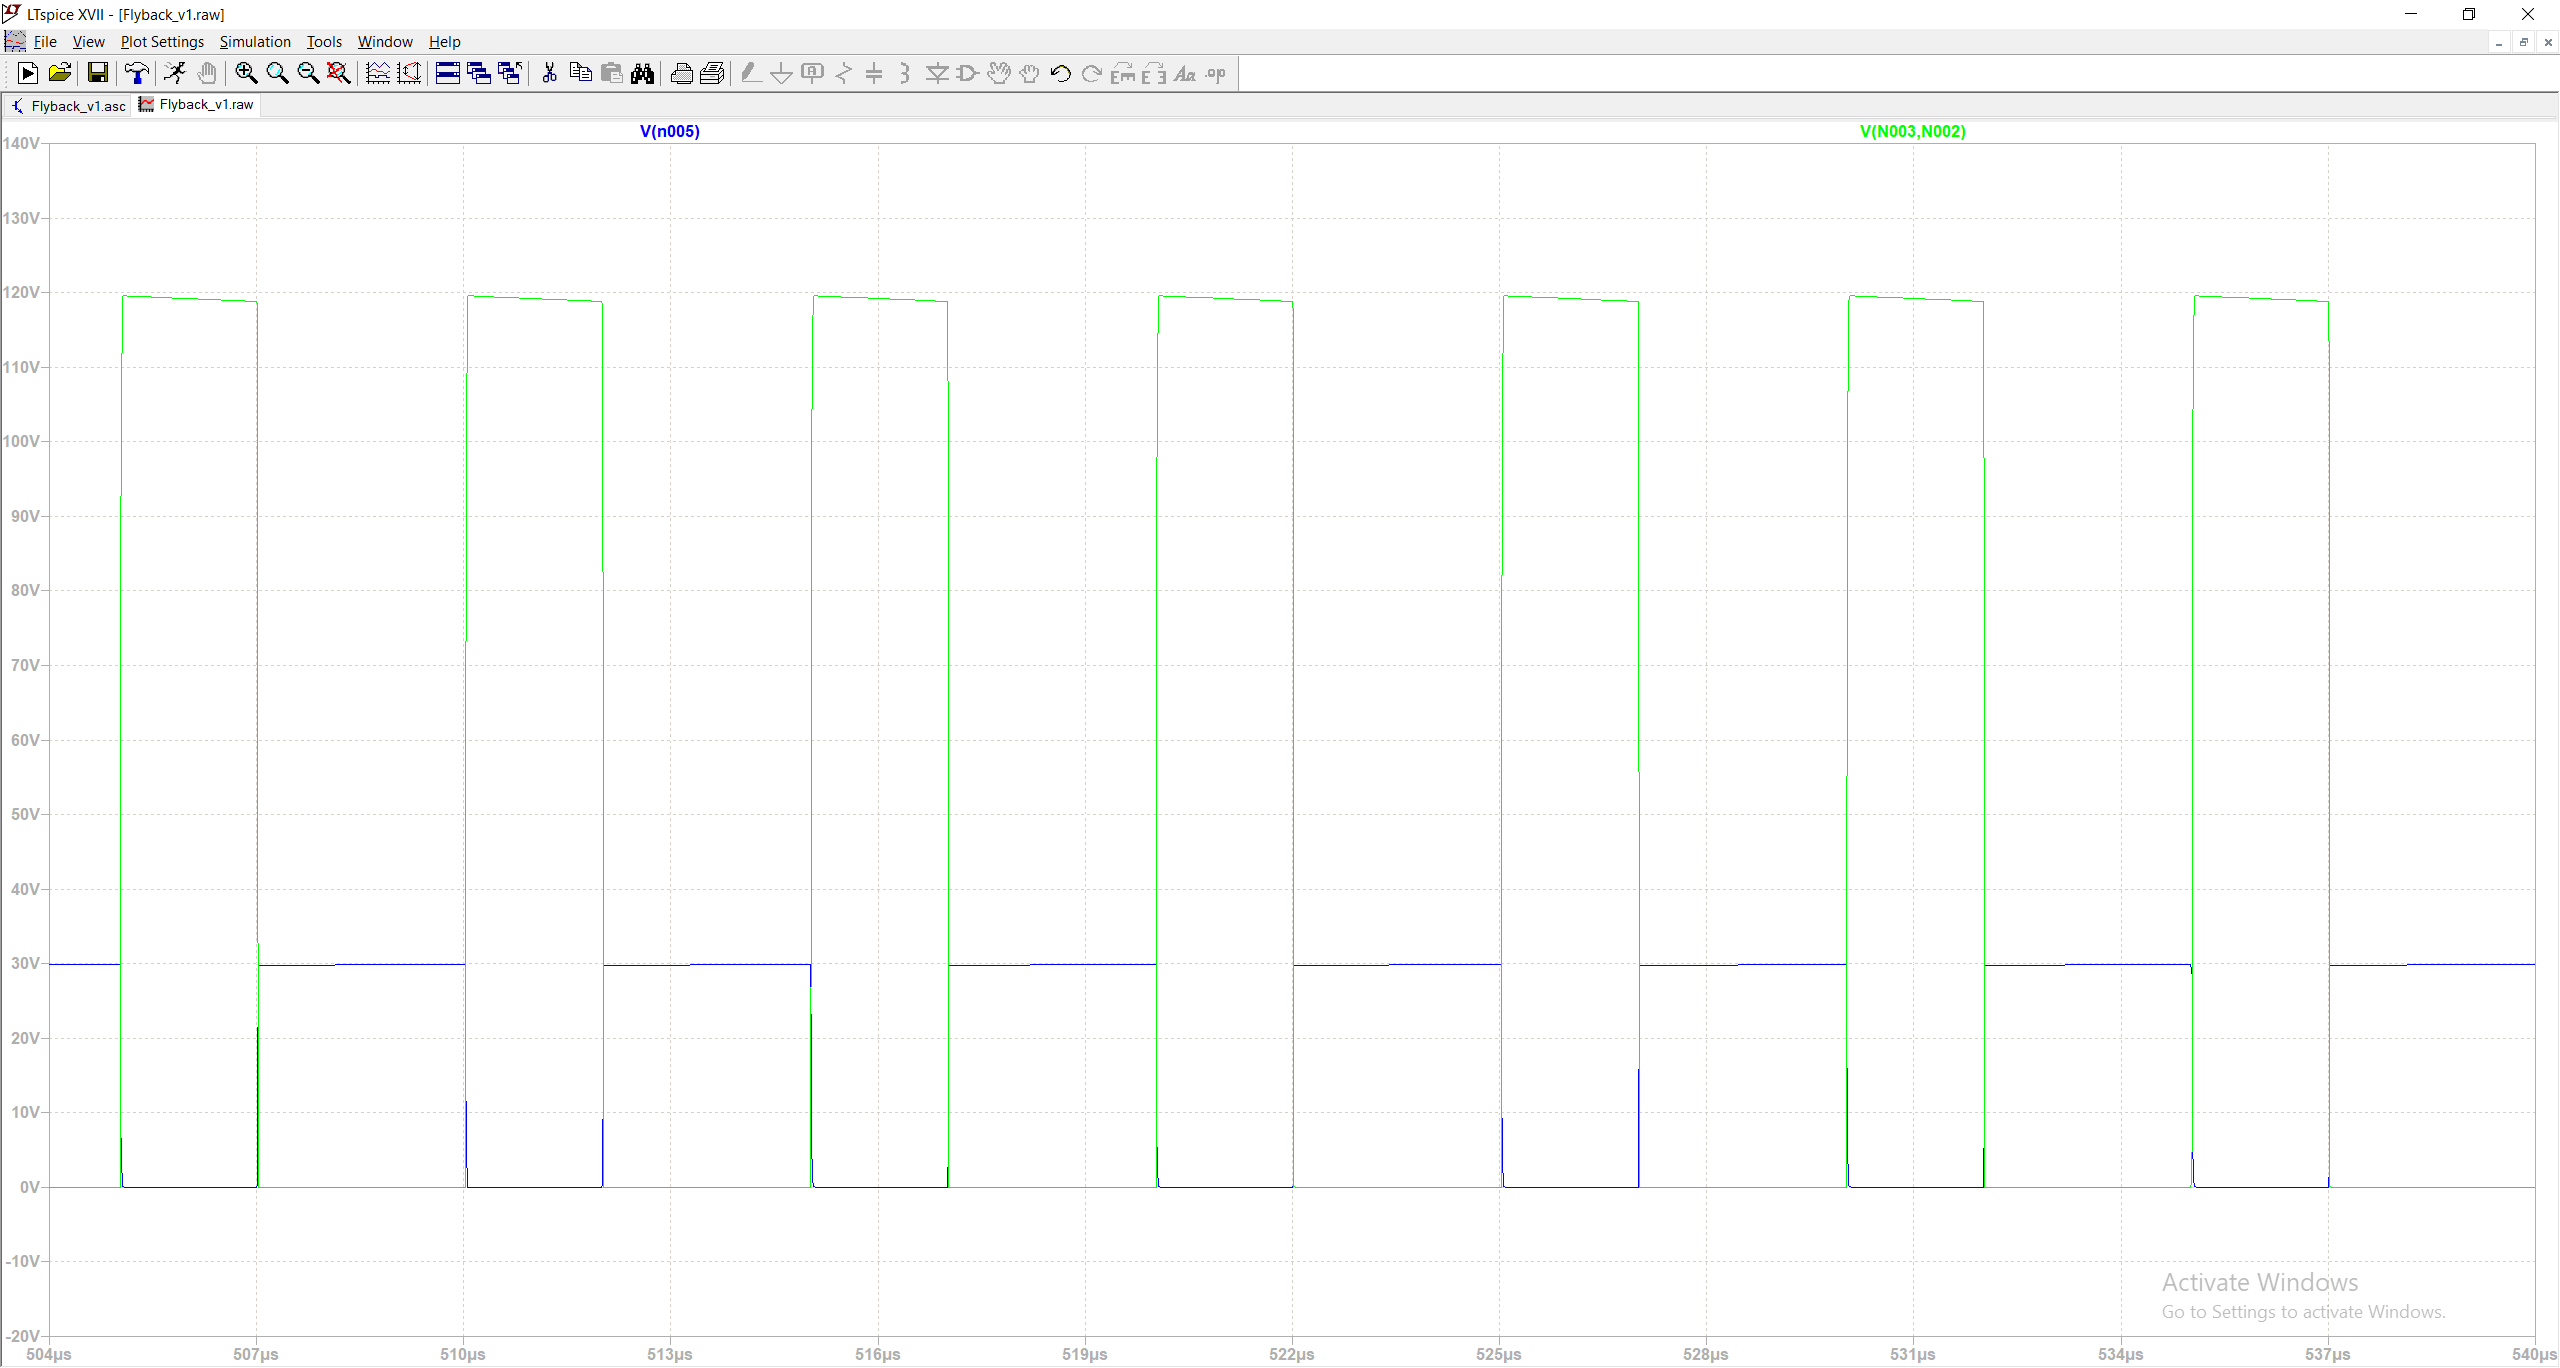
\includegraphics[scale=0.3]{img/Spice_Sim/Ideal/ideal_diode_switch_stresses_Vs_18V.PNG}
        \caption{Diode and switch voltage stresses for 18V input voltage}
        \label{fig:ideal_V_stress}
    \end{figure}

    Finally, the output voltage ripple can be calculated using the equation $\frac{\Delta V_o}{V_o} = \frac{D}{RC f_s} \approx 2\%$. One can see it is consistent with Figure \ref{fig:ideal_Vo}.

    \begin{figure}[H]
        \centering
        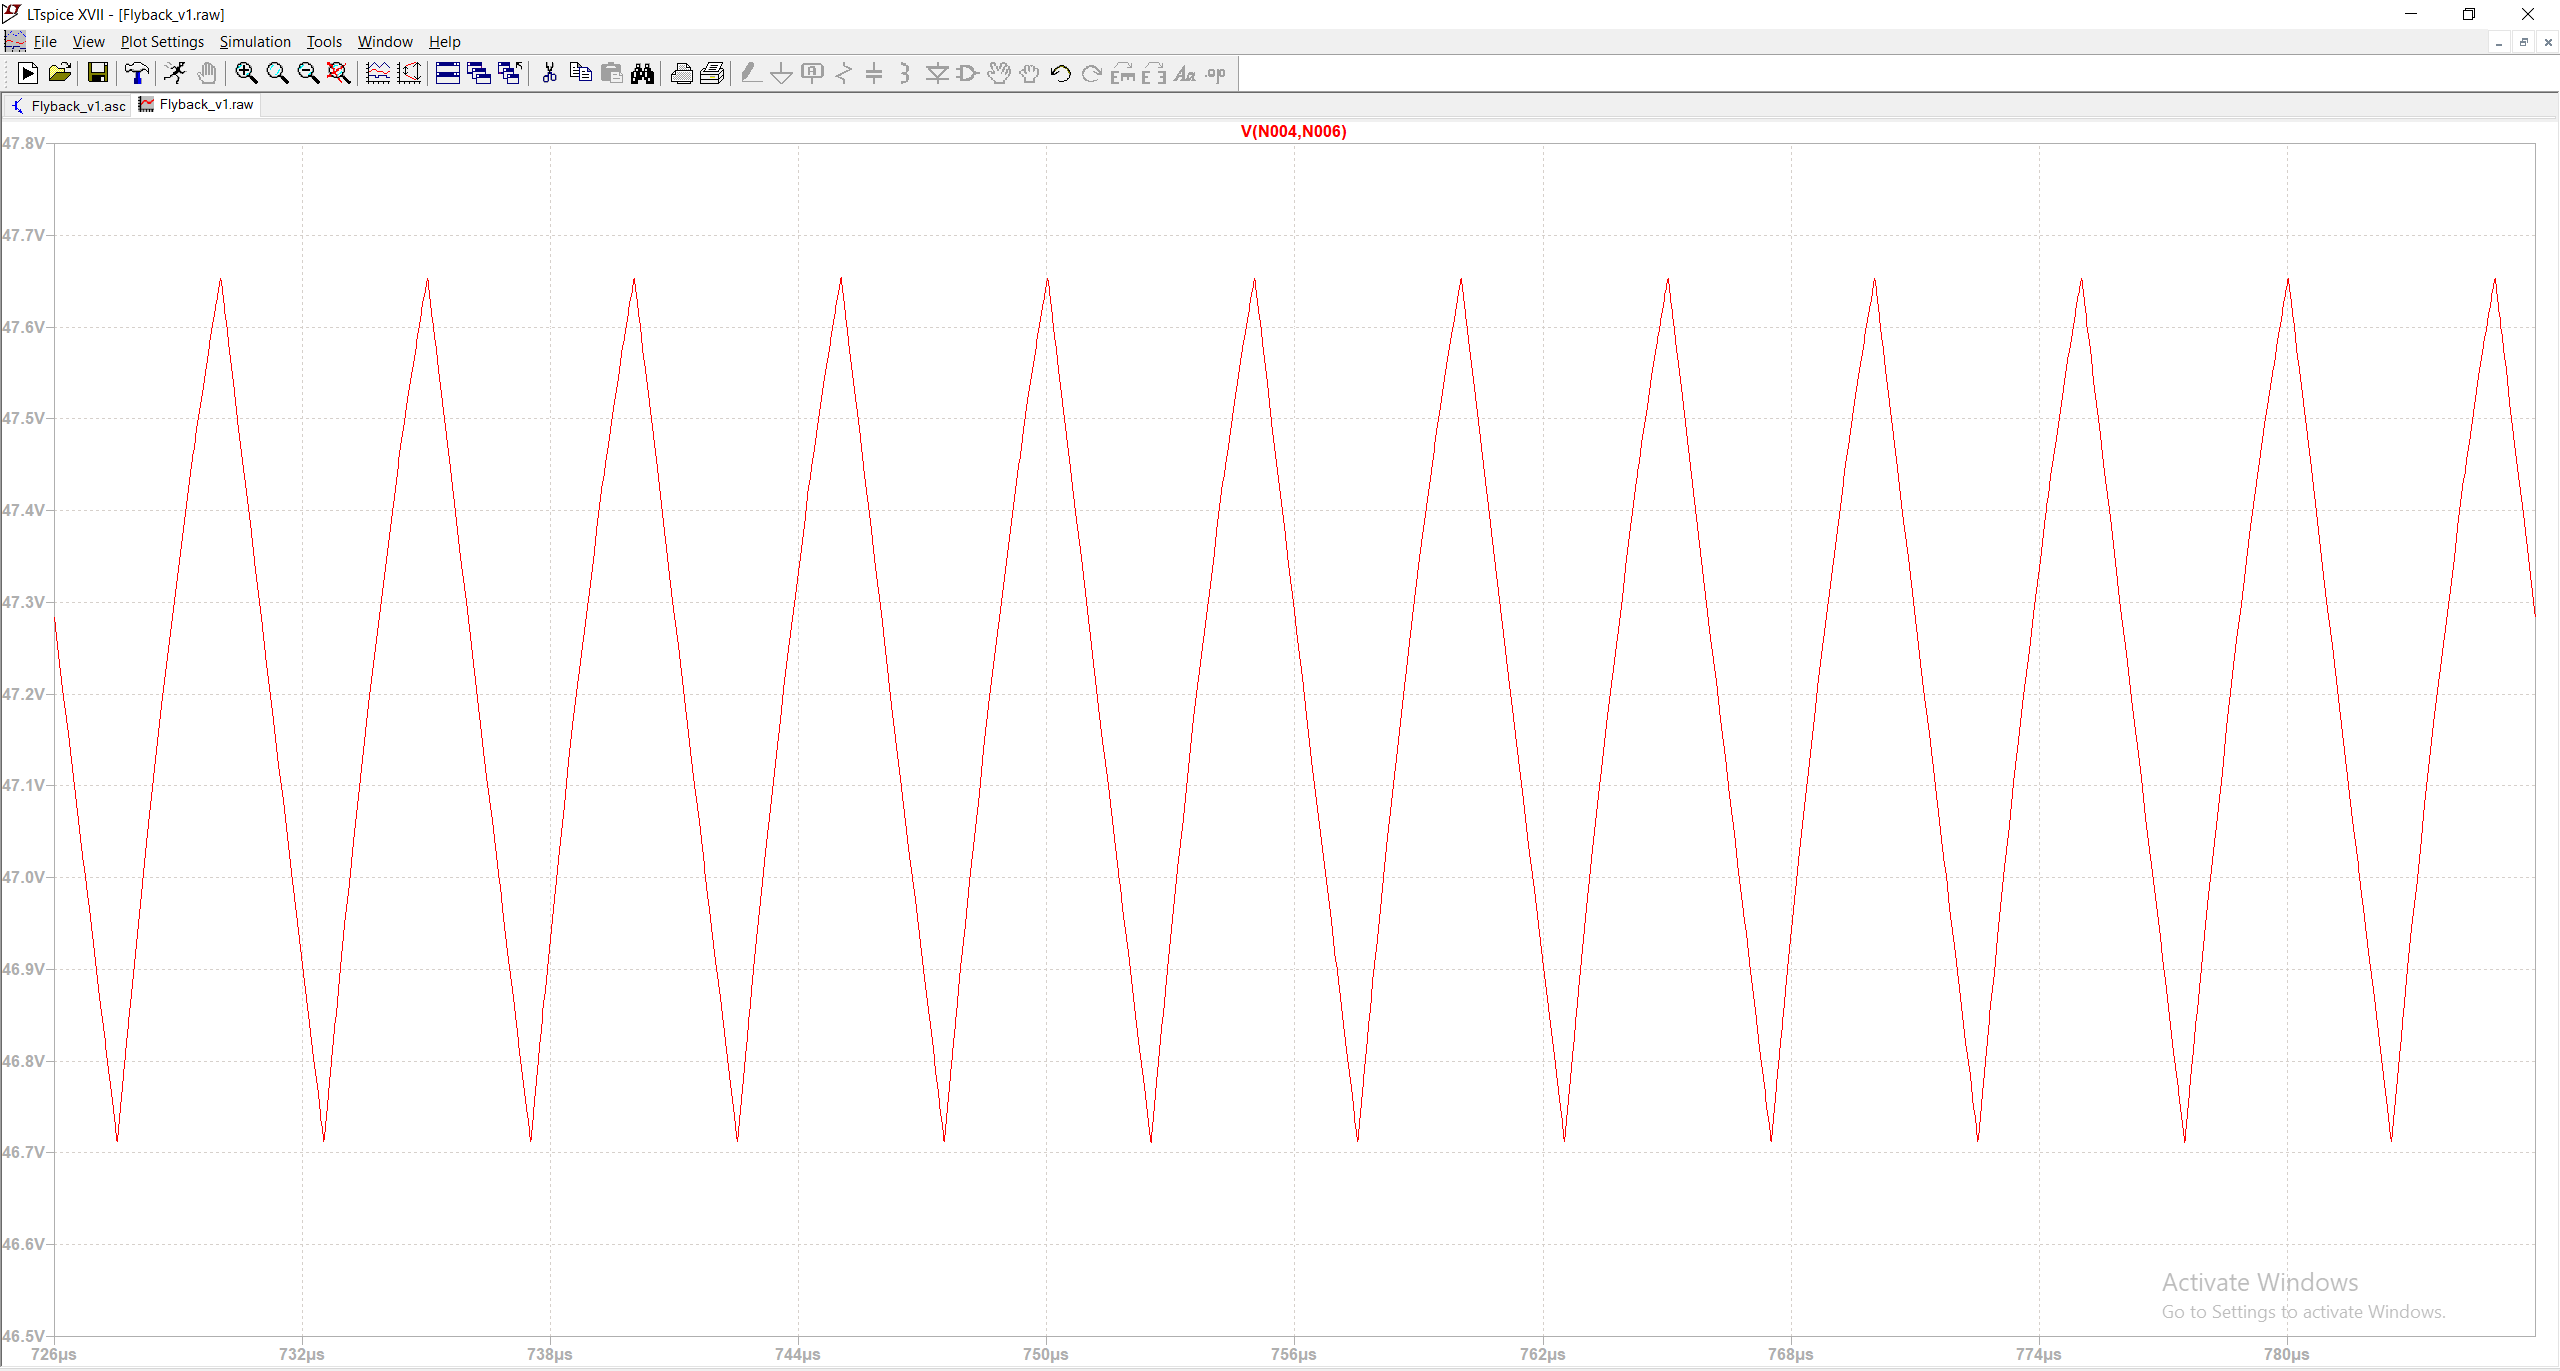
\includegraphics[scale=0.3]{img/Spice_Sim/Ideal/ideal_Vo_ripple_2.6uF.PNG}
        \caption{Output voltage waveform}
        \label{fig:ideal_Vo}
    \end{figure}
    
    \subsection{Non-ideal Simulations \& Snubber Design}
    
    The parasitic effects, primary leakage inductance (which is measured as 3\%), and non-ideal semiconductors are added to the ideal circuit. When we include the parasitic effects and simulate the circuit for 12V input voltage, the leakage inductance creates high voltage stress on the MOSFET during the transition to off-state. This will not blow up our MOSFET as the avalanche energy of the MOSFET is enough to absorb all the energy stored in the leakage inductance. However, since the voltage swing caused by the ringing will be too high, we either had to design a snubber or use a TVS (Transient Voltage Suppression) diode. We made simulations with a TVS diode with 30V rating, which is also included in the schematic. The non-ideal model of the circuit can be seen in Figure \ref{fig:non-ideal_sim_circuit}. \\

    \begin{figure}[H]
        \centering
        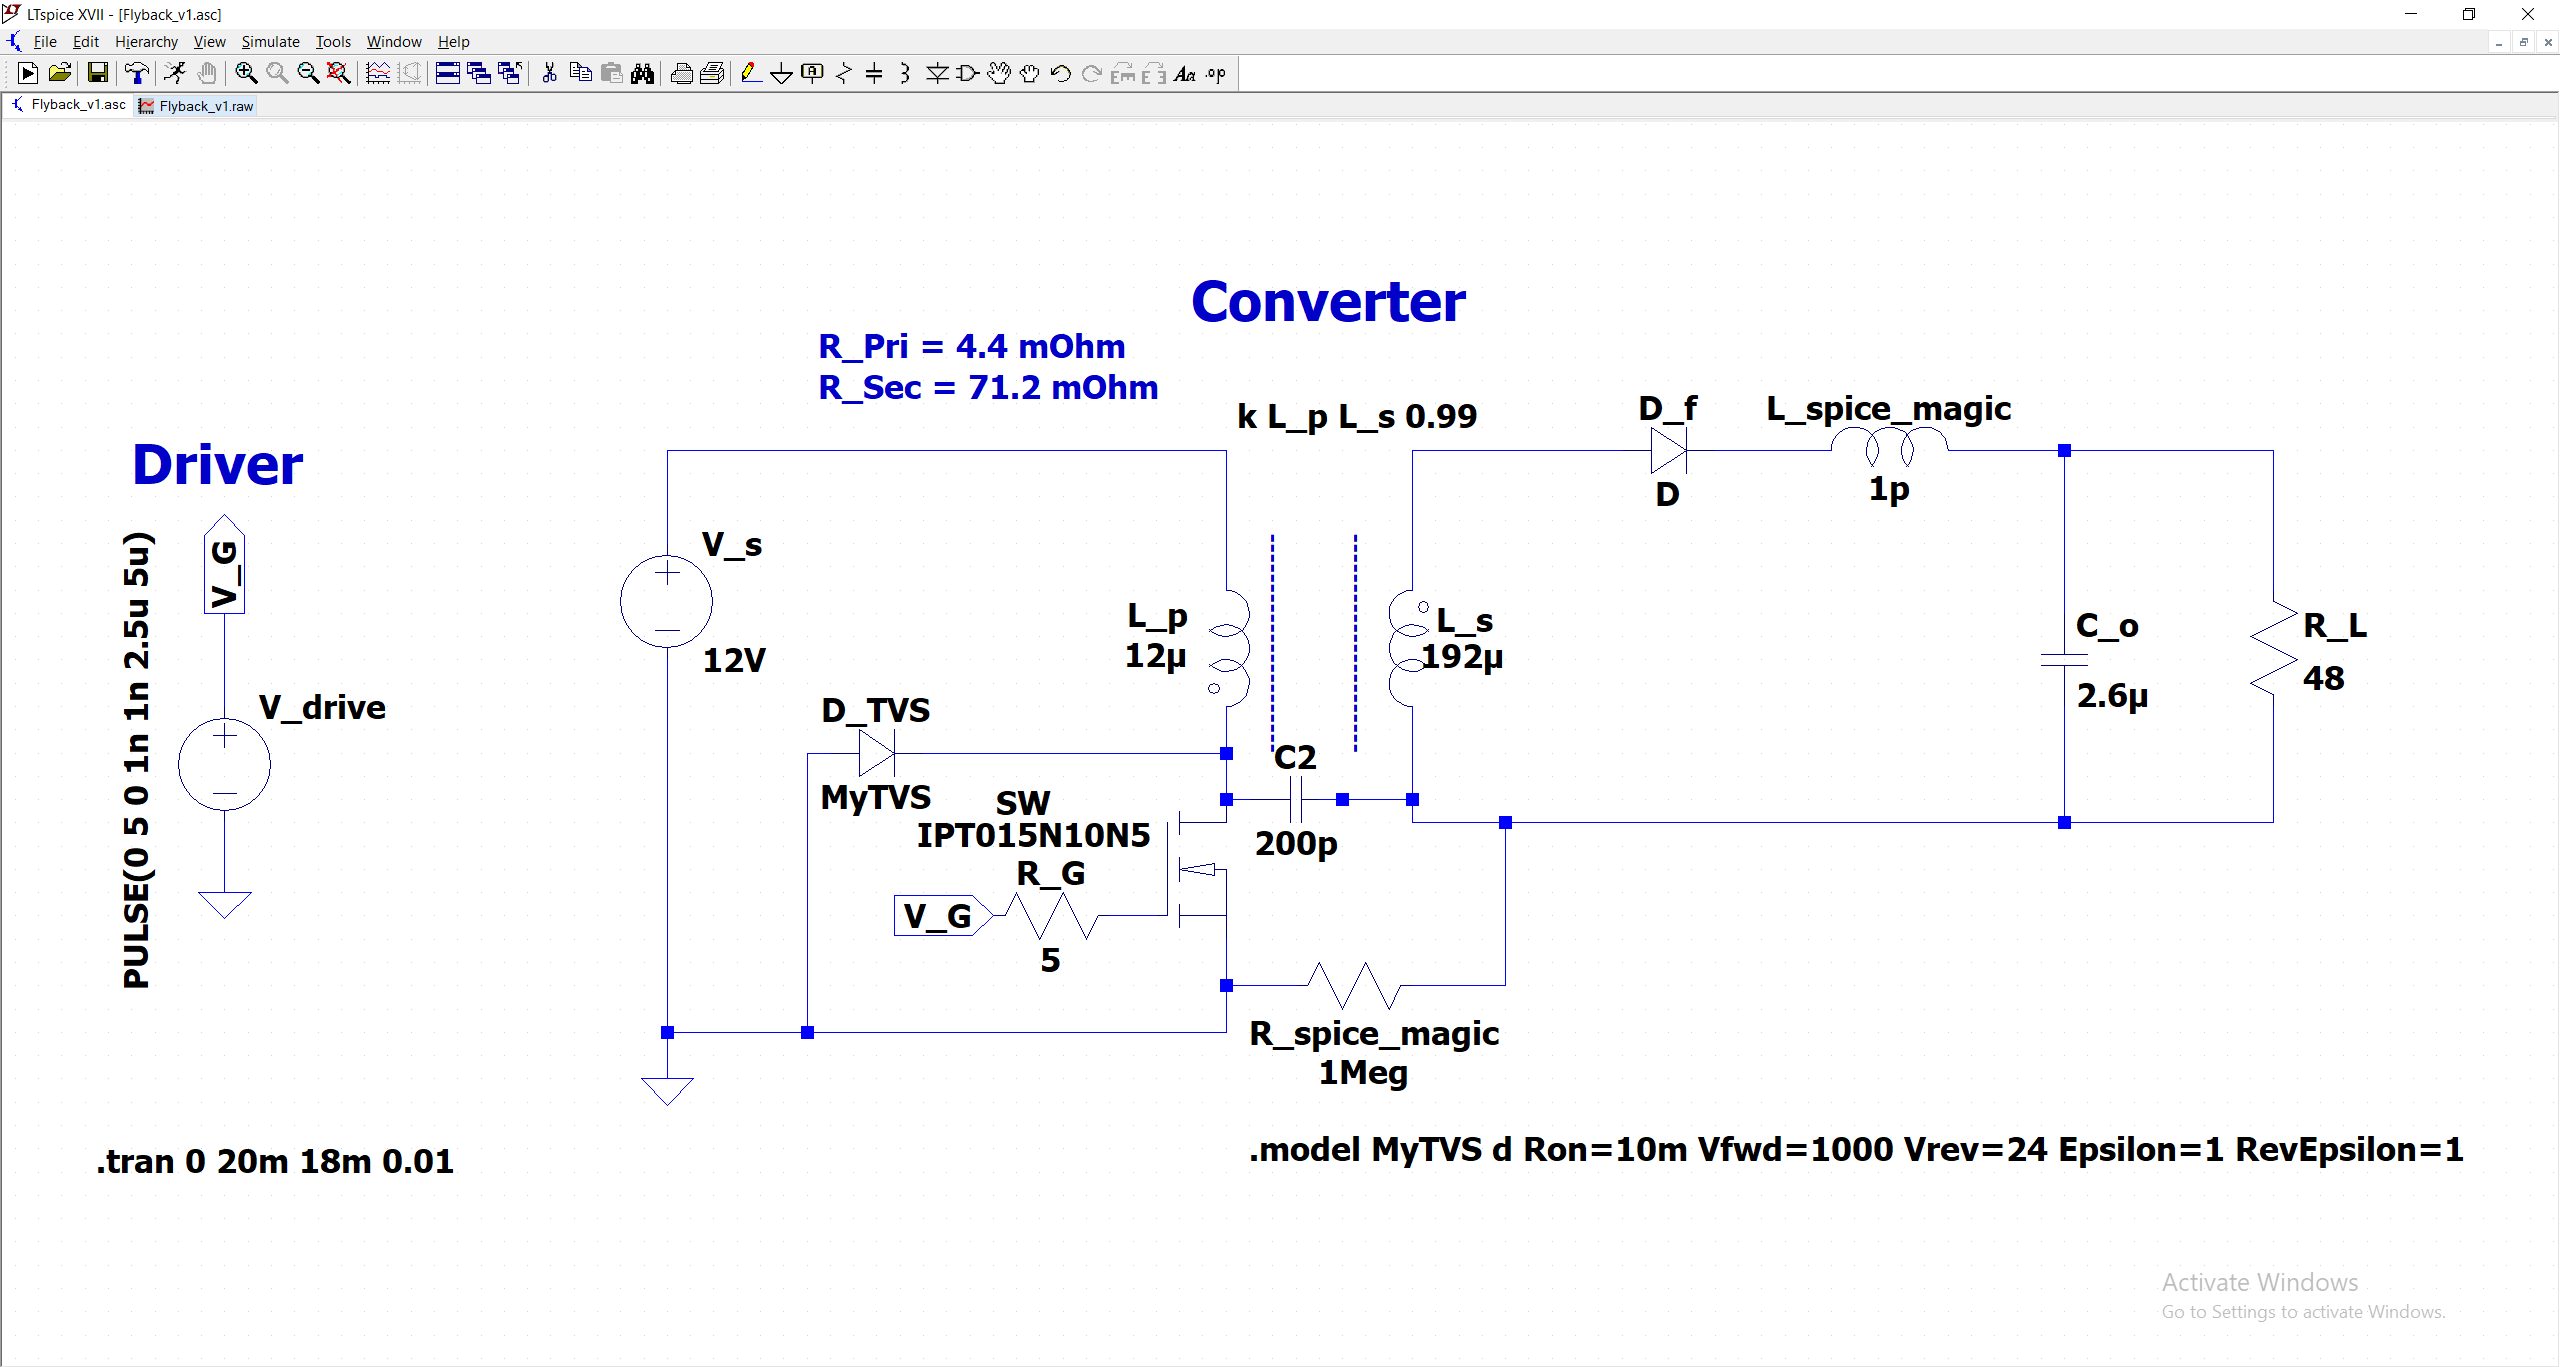
\includegraphics[scale=0.3]{img/Spice_Sim/Non-ideal/non-ideal_simulation_circuit.PNG}
        \caption{Simulated LTspice circuit schematic (non-ideal case)}
        \label{fig:non-ideal_sim_circuit}
    \end{figure}

    Still, there will be some amount of ringing due to the unsuppressed energy. We will see its effect on the transients of the waveforms. The non-ideal simulation results for magnetizing current ripples are given in Figure \ref{fig:non-ideal_Lm_ripple}. The voltage stress on the switch is seen in Figure \ref{fig:non-ideal_V_stress}. Finally, the output voltage waveform is given in Figure \ref{fig:non-ideal_output}. Note that with the duty for ideal case (which is 50\% for 12V input) the output voltage is reduced to 40V. However, since the analog IC does close-loop control, it can increase the duty as much as it is required. Figure \ref{fig:non-ideal_output} shows the output voltage for 12V and 54\% duty, also showing that our circuit is still stable at this operating point.\\

    \begin{figure}[H]
        \centering
        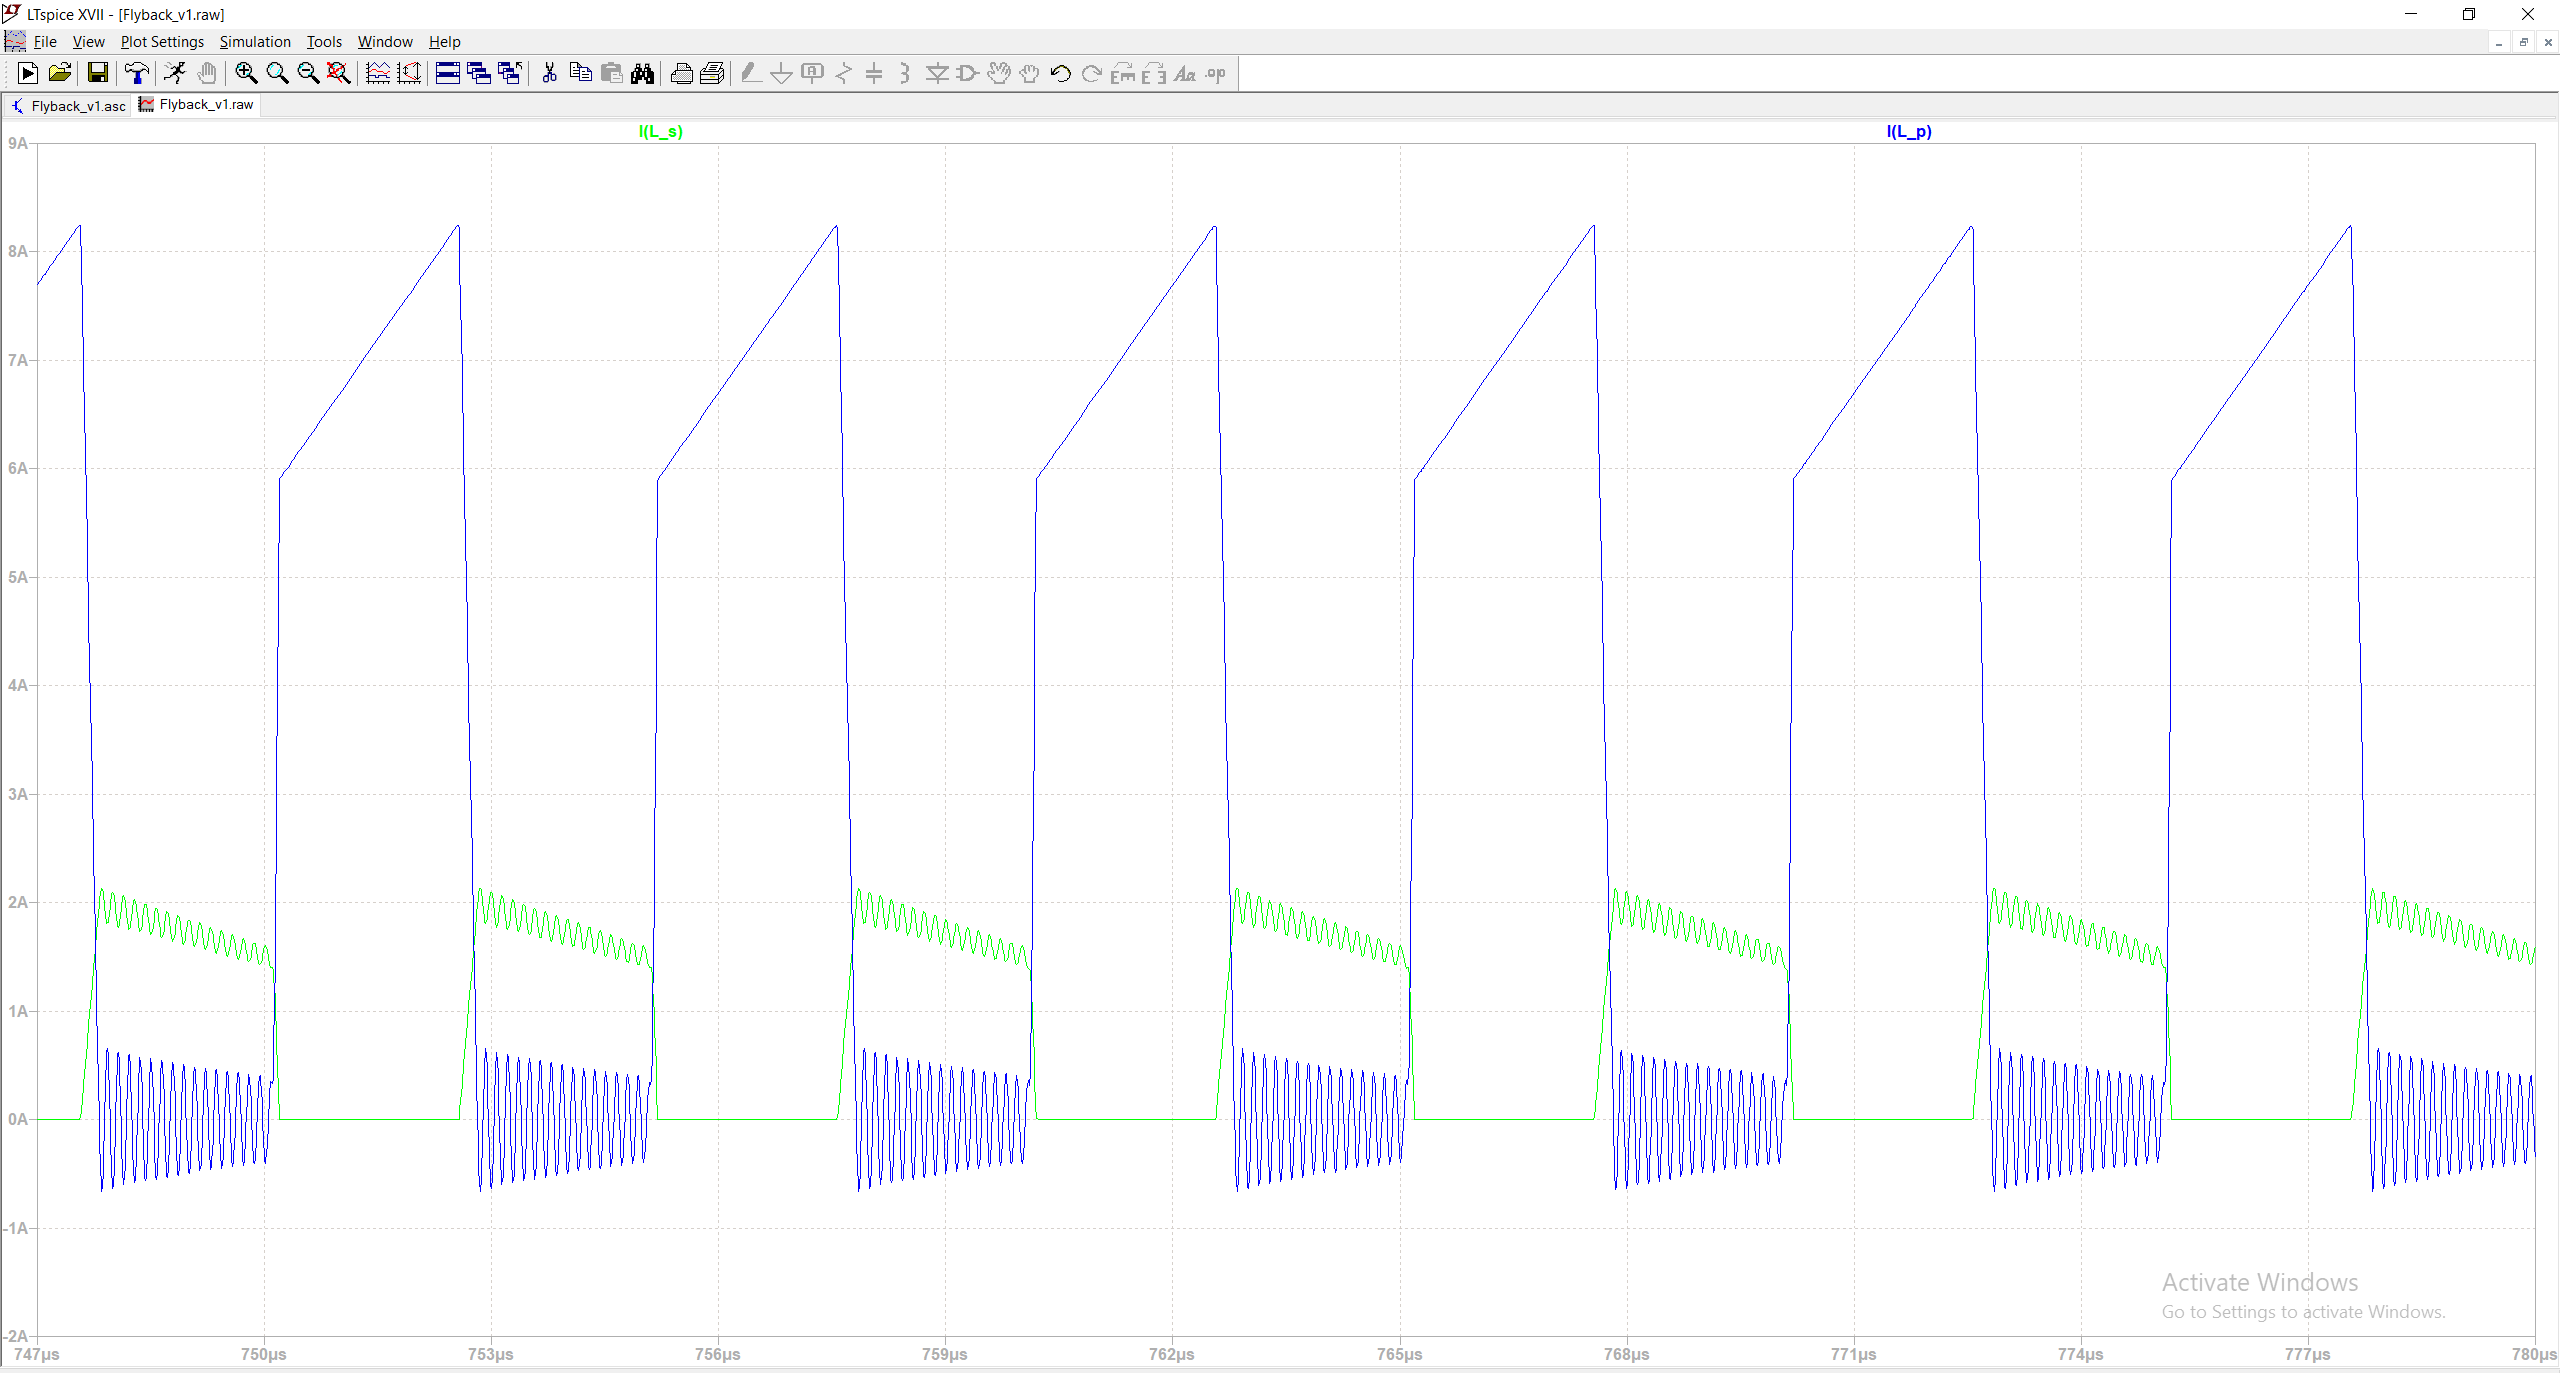
\includegraphics[scale=0.3]{img/Spice_Sim/Non-ideal/non-ideal_Lm_ripples_12V.PNG}
        \caption{Primary and secondary current waveforms for 12V input voltage (non-ideal case)}
        \label{fig:non-ideal_Lm_ripple}
    \end{figure}

    \begin{figure}[H]
        \centering
        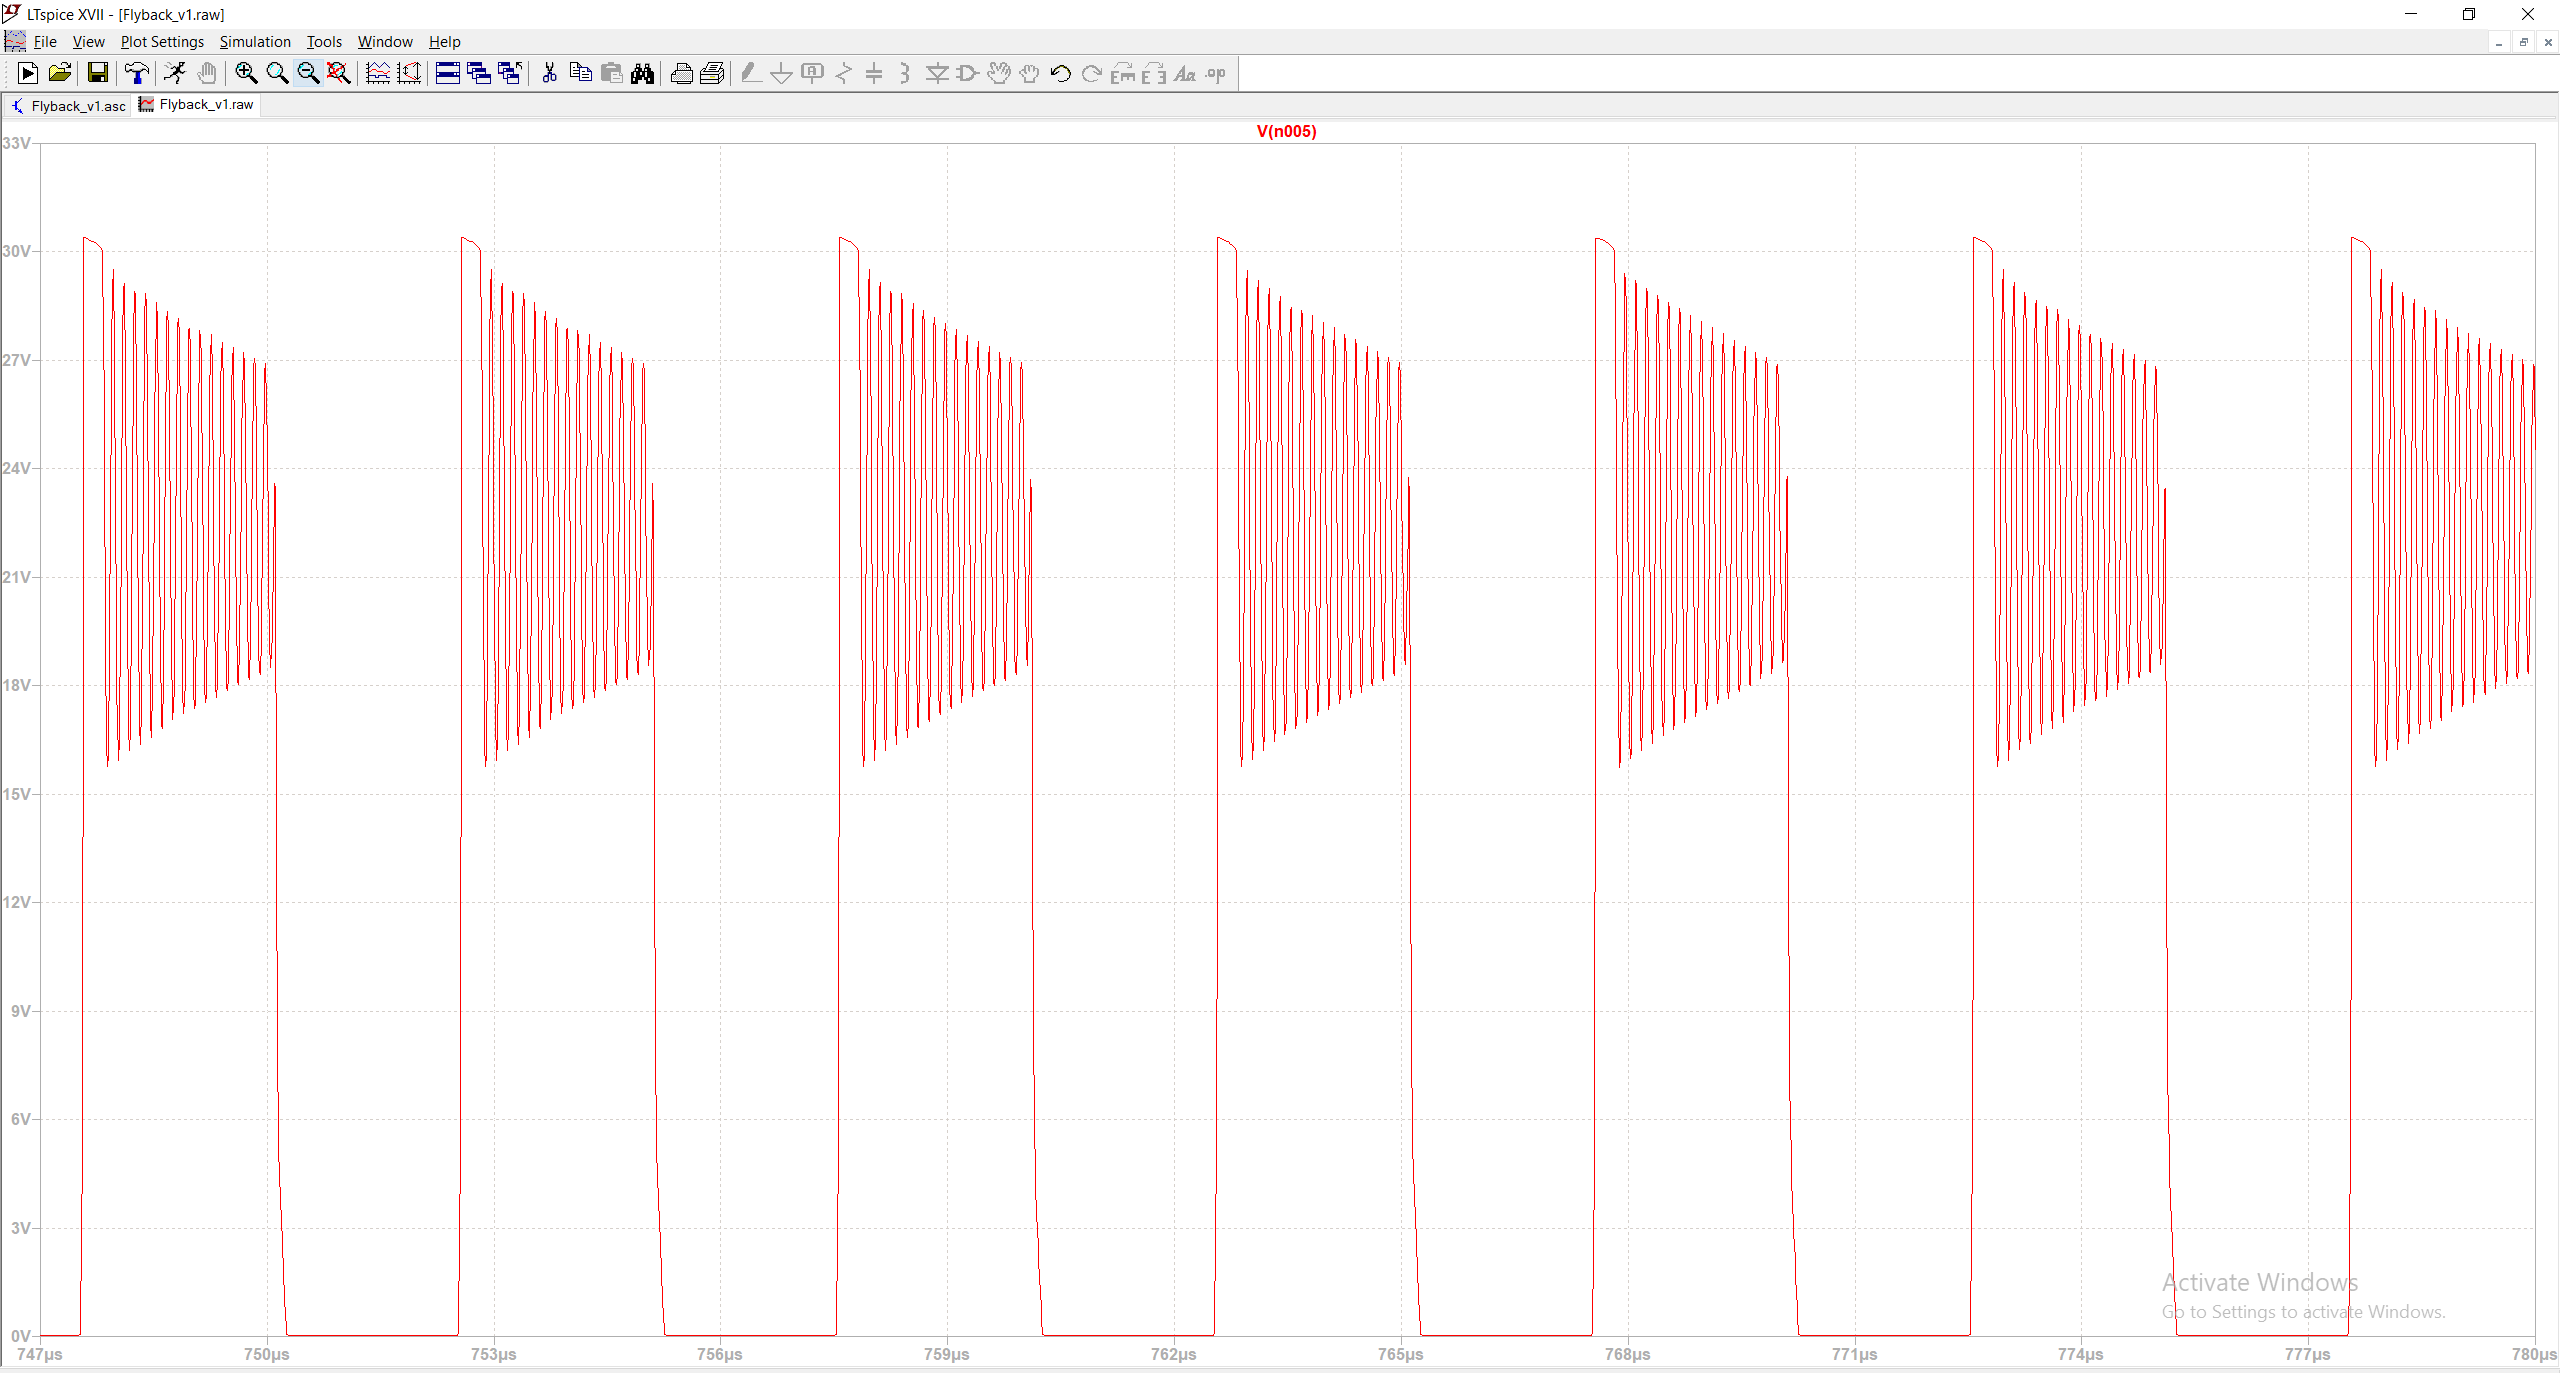
\includegraphics[scale=0.3]{img/Spice_Sim/Non-ideal/non-ideal_diode_switch_stresses_Vs_12V.PNG}
        \caption{Switch voltage stress for 12V input voltage (non-ideal case)}
        \label{fig:non-ideal_V_stress}
    \end{figure}

    \begin{figure}[H]
        \centering
        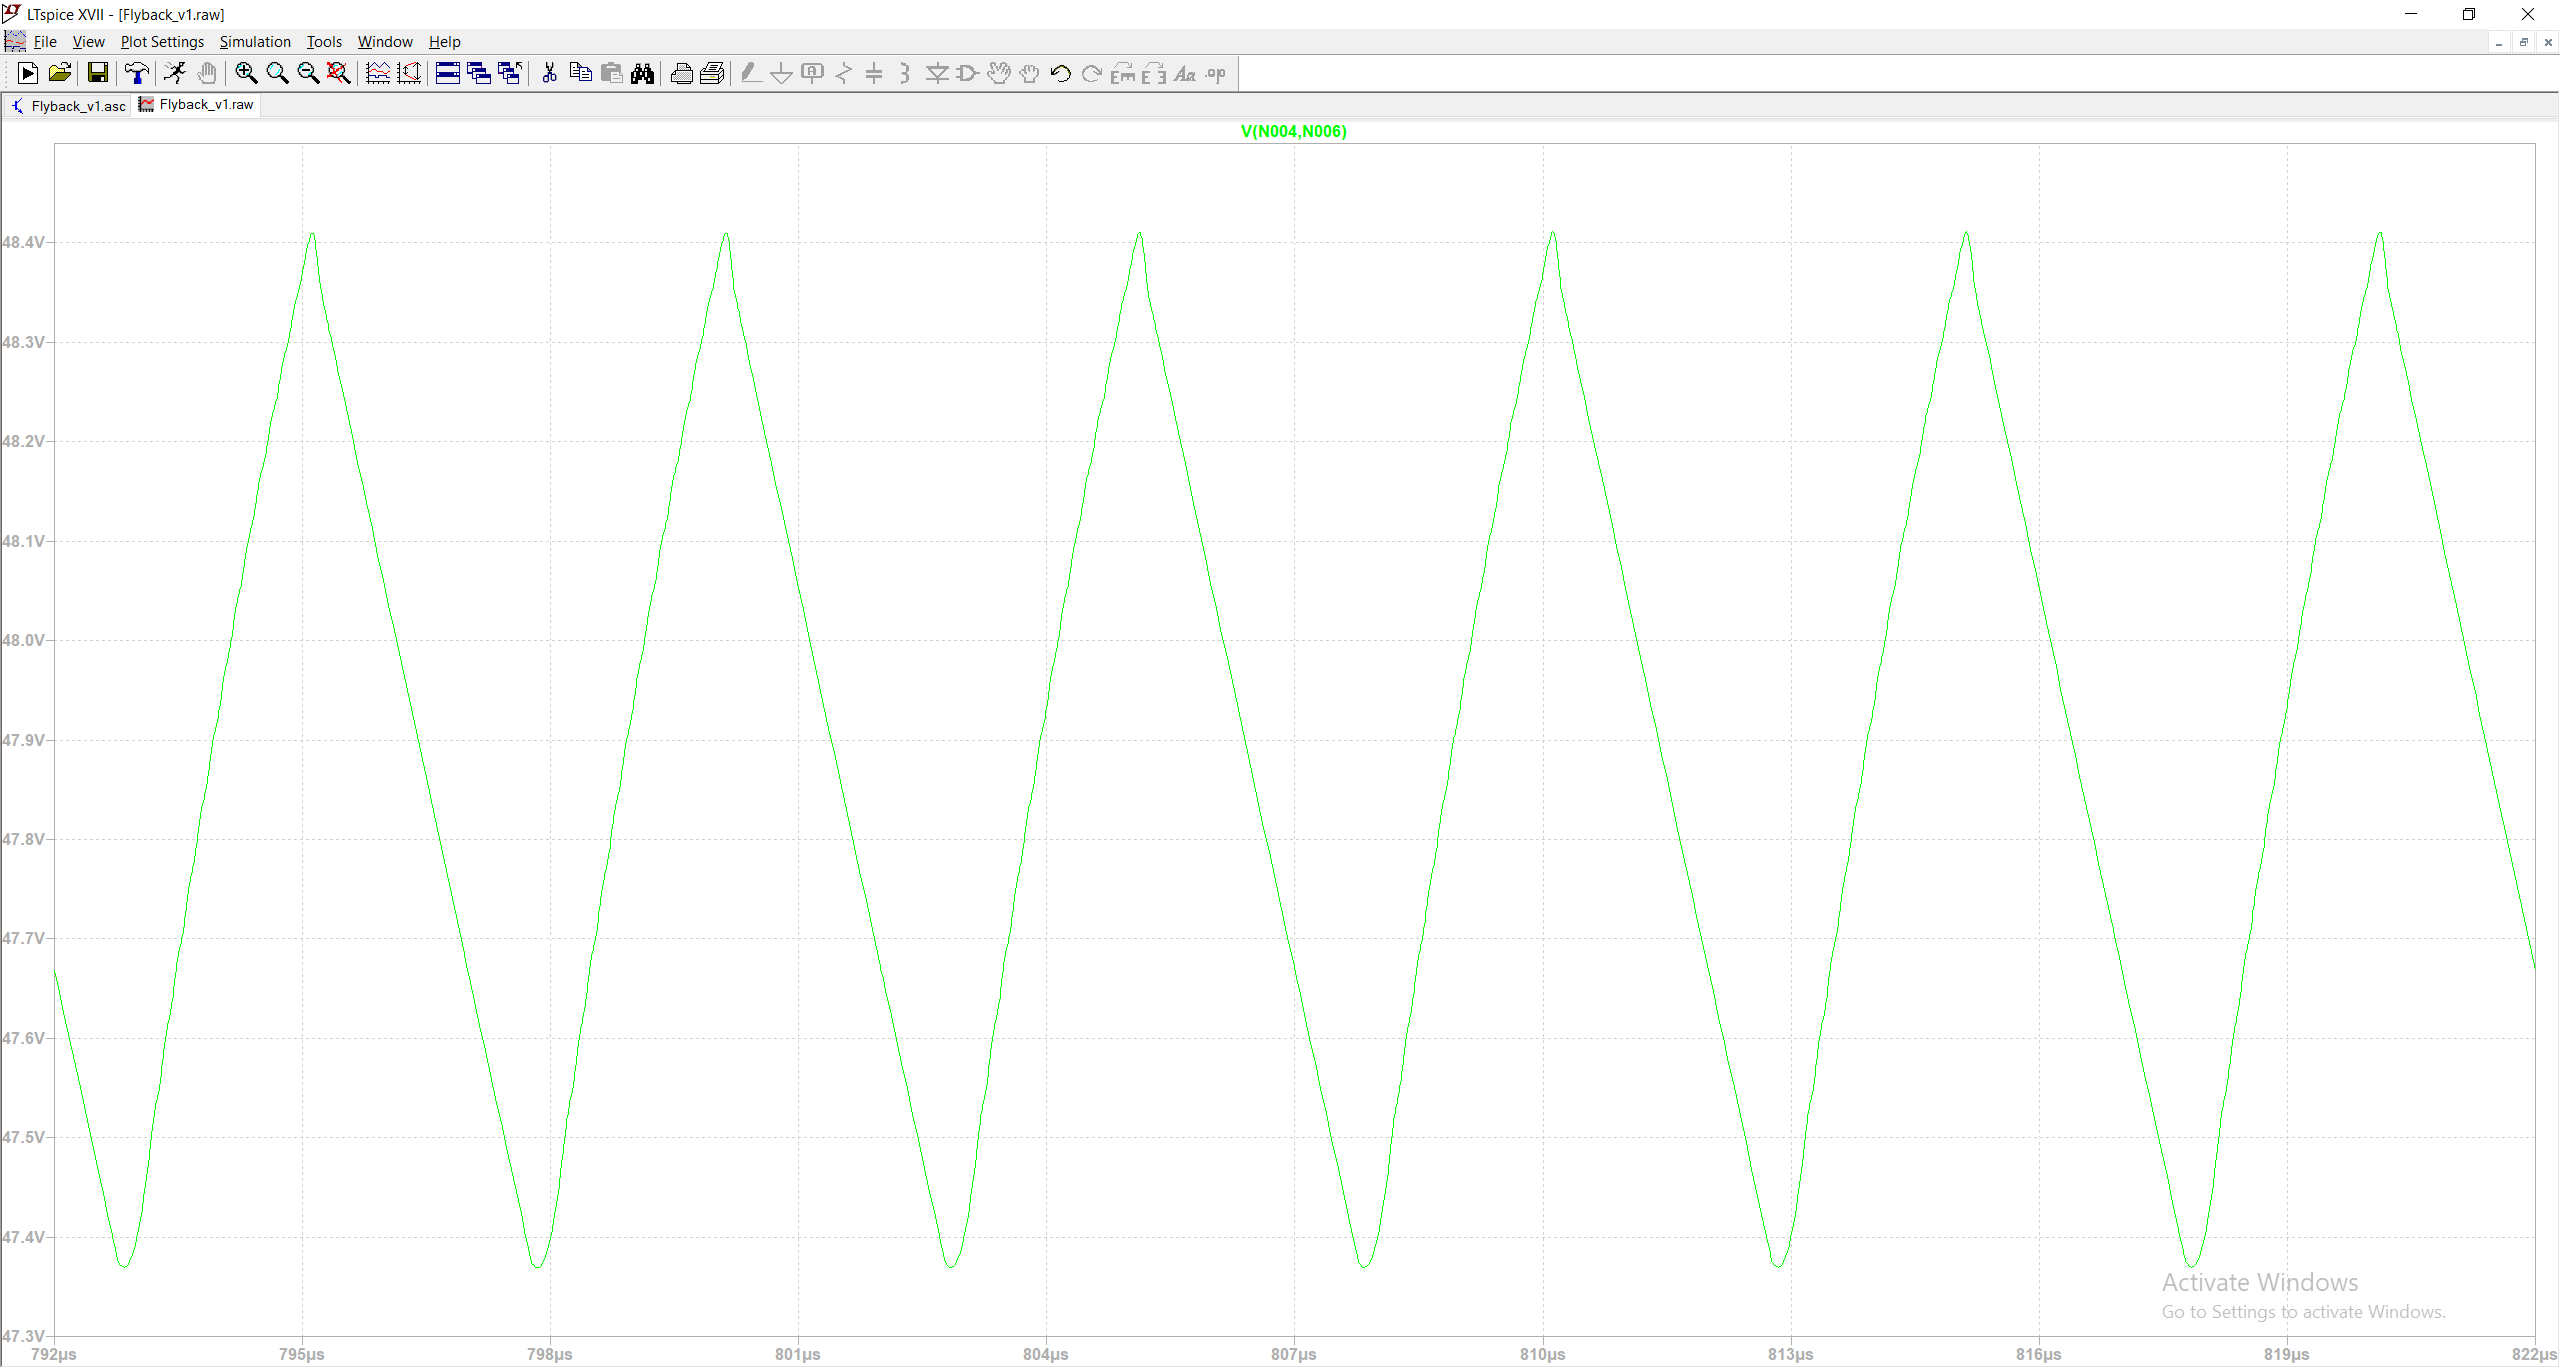
\includegraphics[scale=0.3]{img/Spice_Sim/Non-ideal/non-ideal_output_54duty.PNG}
        \caption{Output voltage ripple with 54\% duty (non-ideal case)}
        \label{fig:non-ideal_output}
    \end{figure}

    However, we realized that this method is not sensible since the energy dissipated on the TVS is extremely high. Hence, we decided to use an RCD snubber. We made many simulations (with various snubber types) to decide on sensible snubber resistance and capacitance values for our case, which limits the ringing to an extent (smaller than 80V max) but also does not increase the losses drastically. The schematic for the final version of the snubber in the primary side is given in Figure \ref{fig:snubber}. The ringing on the MOSFET voltage for these values are given in Figure \ref{fig:snubber_ringing}.

    \begin{figure}[H]
        \centering
        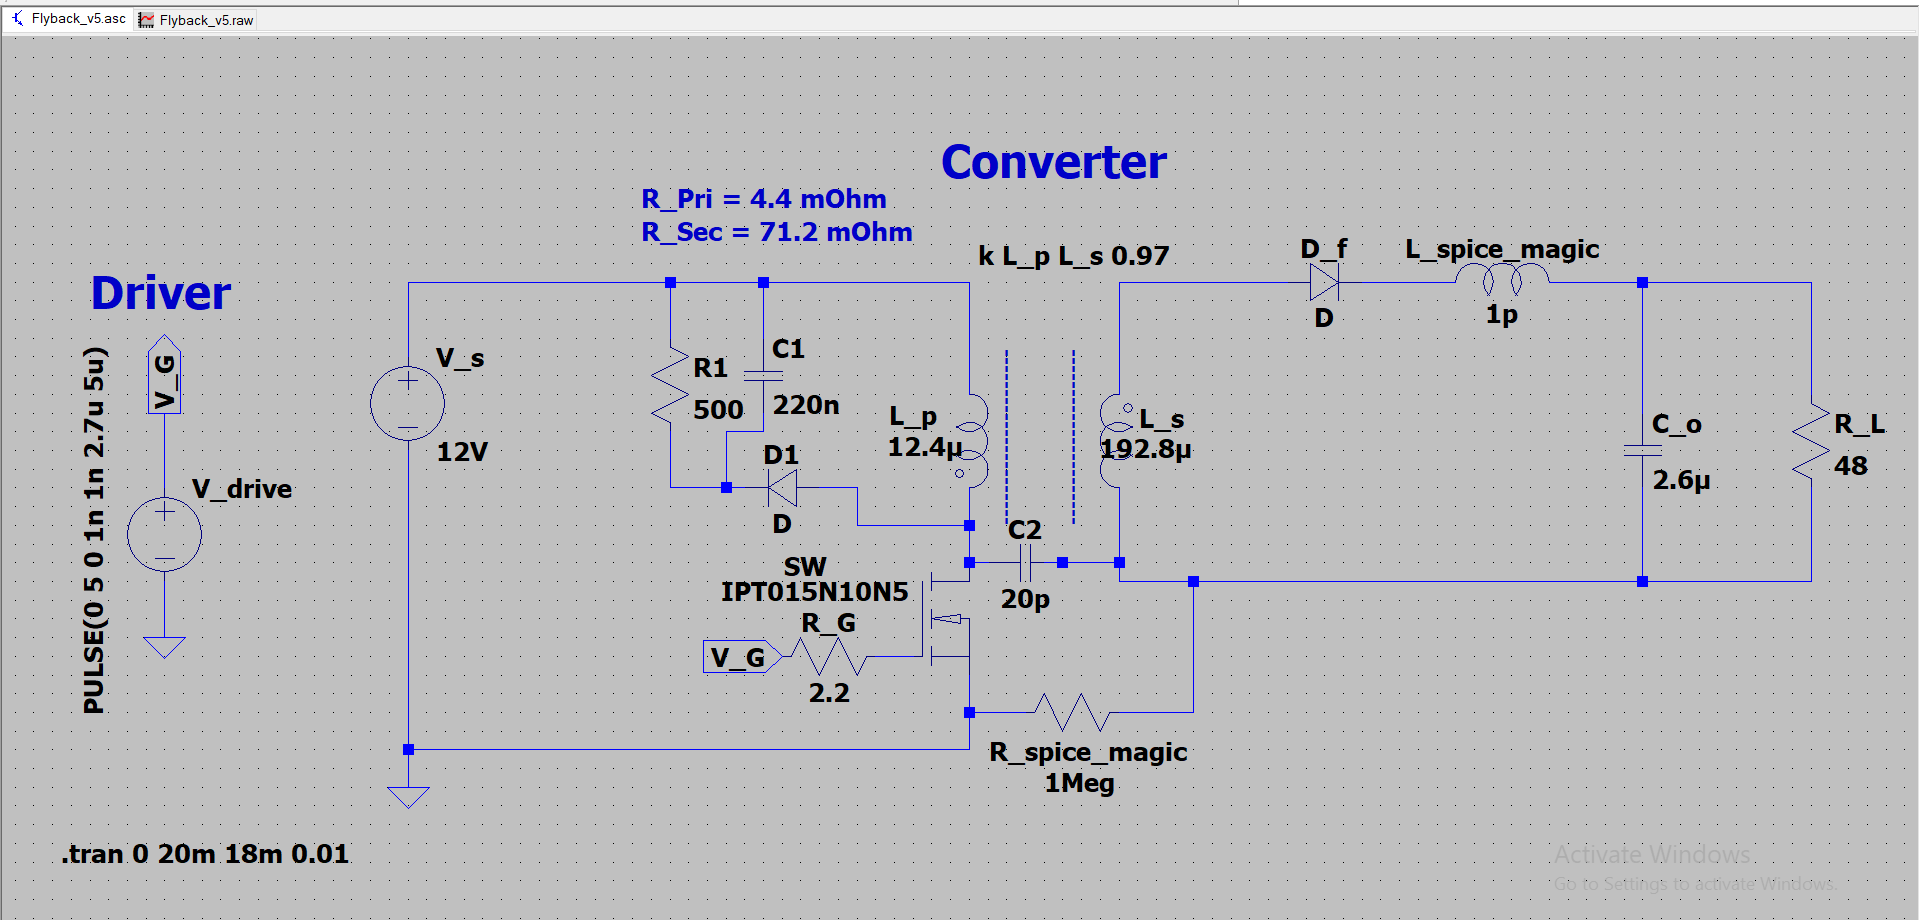
\includegraphics[scale=0.4]{img/snubber_schematic.PNG}
        \caption{Snubber circuit simulation schematic for the primary side}
        \label{fig:snubber}
    \end{figure}

    \begin{figure}[H]
        \centering
        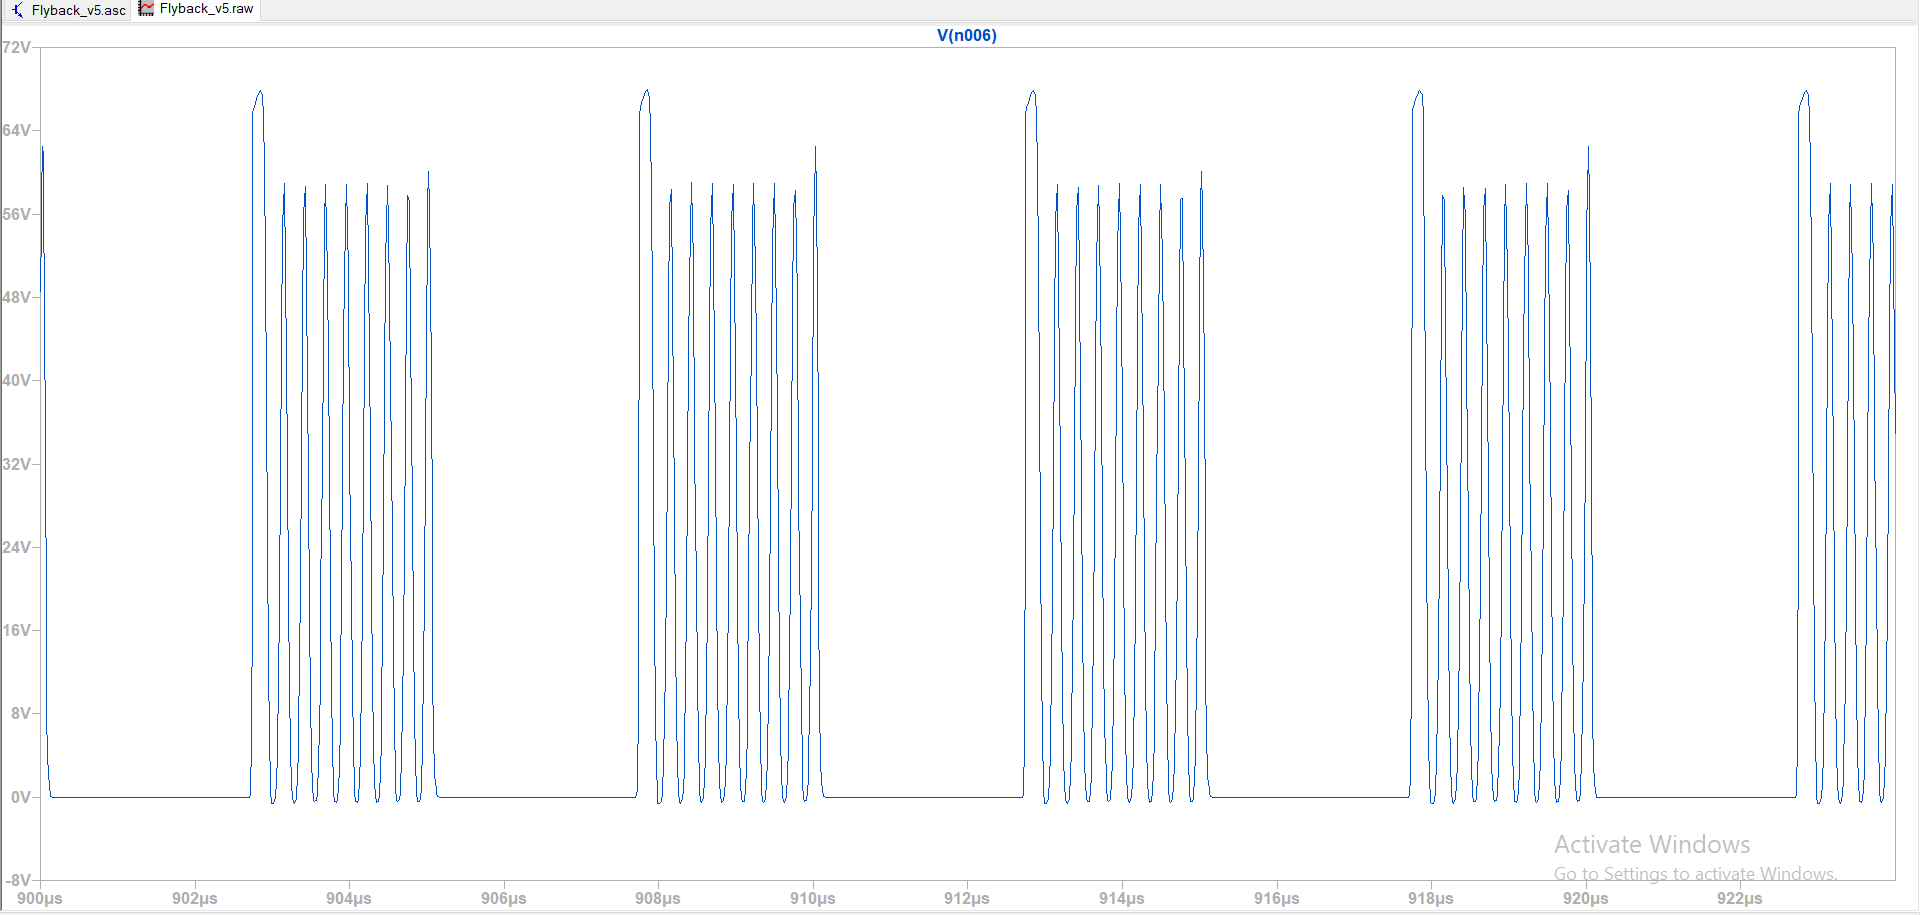
\includegraphics[scale=0.4]{img/snubber_ringing.PNG}
        \caption{Ringing on the MOSFET with the RCD snubber (simulation results)}
        \label{fig:snubber_ringing}
    \end{figure}

    We can see that there is still a lot of ringing, but considering our MOSFETs voltage ratings (100V with high avalanche rating) this is not harmful. Furthermore, the Spice simulation somehow creates more ringing; possible parasitic or other effects damps the ringing very fast in the real case, as seen from the experiments we did. The reflection of this ringing voltage may create voltage stress on the secondary side diode. Hence, we also added an RC snubber in parallel to the secondary side diode. \\

    The losses on the snubber in the simulation is 5.93W, which is significantly high. However, this is due to the energy stored in the leakage inductance before the turn-off moment of the switch, due to high primary side peak current. The stored energy in the leakage is equal to $\frac{1}{2}Li^2$ and if all of the energy in the leakage is spent on the snubber, the power dissipated is equal to $\frac{1}{2}Li^2f_s = 3.72W$ for 10A peak current (which is the chosen limit for our peak current mode controller, for the ideal case). Hence, we saw that a large loss in the snubber is expected for this flyback topology, for an application with high input side current. A two switch topology, a zero-current switching topology, or something else might have been more appropriate for this case in terms of losses. Furthermore, the switching frequency may be reduced to a much lower value to lower the snubber losses.

    \subsection{Controller Simulations}

    Controller simulations also take part in the LTSpice environment. The controller is the main part of the simulations, however exact spice model is unavailable, as a solution a counterpart model LT1243 is used which has the same working principle and parameters. 
    
    \begin{figure}[H]
        \centering
        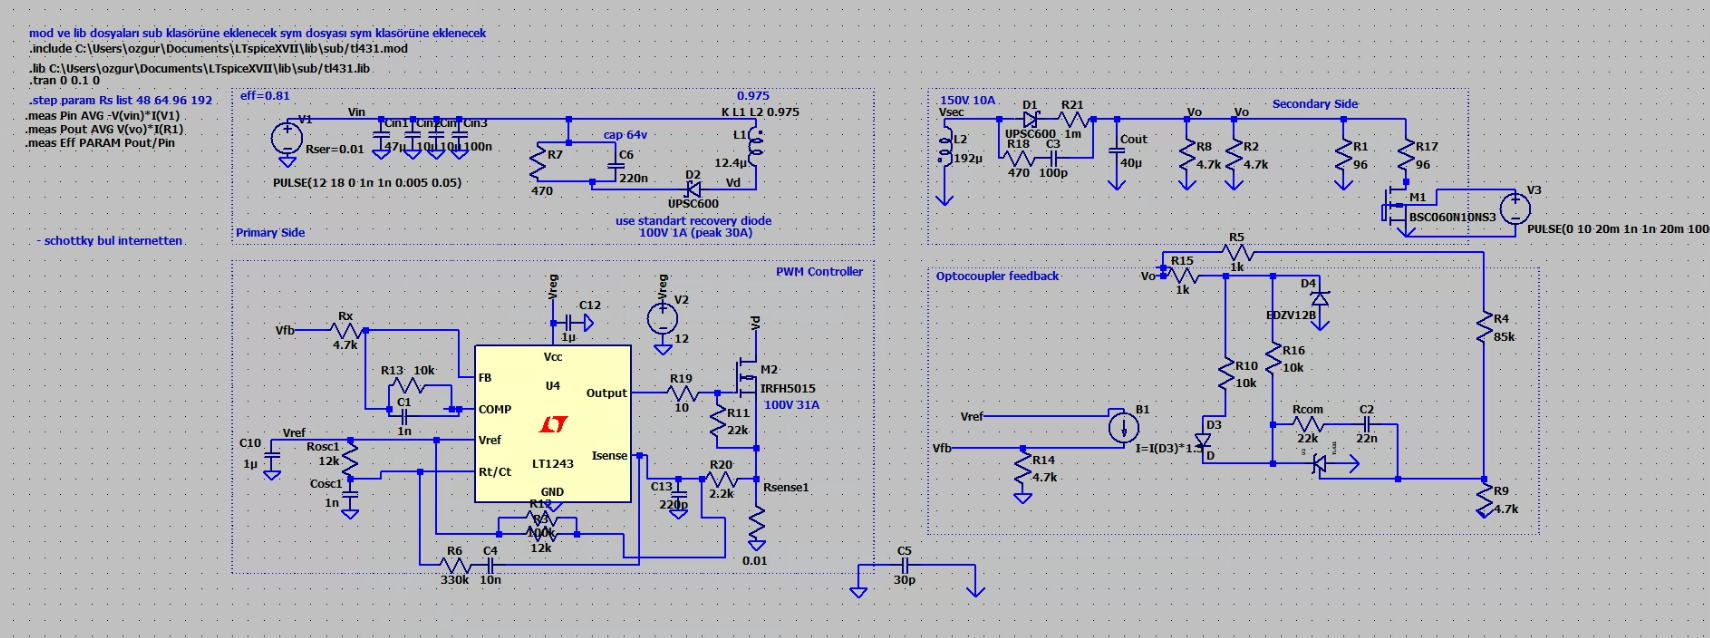
\includegraphics[scale=0.4]{img/controller.png}
        \caption{Controller integrated simulation in LTSpice.}
        \label{fig:controller}
    \end{figure}

     Starting with the secondary side. The compensation circuitry is first designed allowing the output to set the desired voltage. Later in the transient case the output voltage is compensated with the Rcom and C2. These values depend highly on the converters transfer function and operation range and are found via iterative testing.\\

    The optocoupler is used in analog fashion, and proper biasing with R10 is required. The D4 zener diode is used to set the high voltage to a constant 12V and the TL431 at the bottom changes with its feedback function to alter the voltage level at the cathode of the optocoupler diode.\\

    The optocoupler is modelled with a behavioral current source with a gain factor similar to the one that is expected to be used. A generic optocoupler also works in this configuration but if not found this is a method to emulate the workings. \\

    For the primary part this is where the active switching elements are used and controller takes place. The timer configuration for setting the switching frequency worked as expected with the formula mentioned before. Compensation part is continued for the primary side however a generic design is enough which is 10k for R13 and 1 nF for the C1. Vcc of the controller is regulated with a 12V voltage regulator that is LM78m12 and it is capable of supplying the controller and mosfet even for high frequencies such as 200 kHz. \\

    Due to the high input currents, the shunt resistor is selected as 10 milliohms and expected to dissipate around 1W of power when RMS current is about 7.5 Amperes with peaks up to 12 Amperes. For higher resistance values for the shunt resistor, the power loss increases. The controllers peak current limit is however set to 1 volts meaning that the shunt resistor with 10 milliohms is unefective for this configuration with resulting in a sensed voltage of 0.12 volts at peak current. The solution is biasing the current reading pin of the controller. A resistor that is connected between the reference voltage pin and the current sense pin effectively rises the sense value with that a current limit can be set. A quick note on that, the current sense filters resistor and the biasing resistor that mentioned just previously is used together to set the biasing hence the current limit can be set. \\

    The filter on the current sense is important in order for the controller since high frequency noises can introduce extra turn off signals for the mosfet hence the switching frequency might be altered. The used filter is not a harsh one but softer filters introduce aforementioned unexpected outcomes hence the filter is important at the current sense. \\

    After the values for the components are set, the transformer is changed to the non-ideal case and the the results stayed as expected. Then the transient tests are done in simulation environment with varying input voltage and changing the load. A single time sequence with varying input voltage and changing output load is shown below. \\

    \begin{figure}[H]
        \centering
        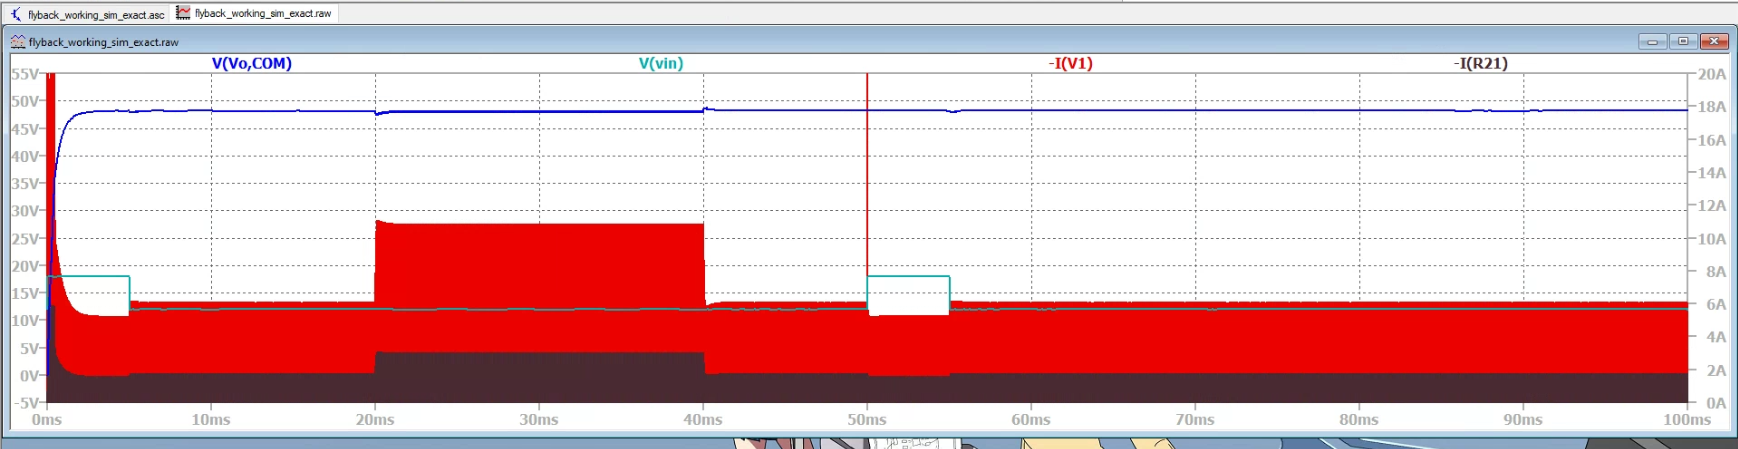
\includegraphics[scale=0.4]{img/sim.png}
        \caption{Transient simulation capturing all the necessary aspects.}
        \label{fig:sim}
    \end{figure}

    

    

    
\section{Component Selection}

    Aside from the core, which was luckily found, there are 4 components to choose.
\begin{itemize}
    \item IC: UC3843AN \cite{ic}. 

    The criteria in choosing the PWM controller IC were that it is able to operate at out input voltage range so that no auxilliary windings are necessary and that it has no PWM limit. 

    UC3843AN satisfies both constraints. It operates at voltages higher than 8V and can provide 100\% duty cycle. A separate feedback network can be built and connected to the IC for closed loop operation. Moreover, it can provide up to 1A gate current. 

    \item MOSFET: CSD19534Q5A \cite{mos}

    The most important criteria in MOSFET selection are rated voltage and current as well as slew rate. CSD19534Q5A has 100V rating in addition to having 10A current rating. This MOS also benefits from low losses thanks to $12.6 m\Omega$ on resistance.  

    \item Diode: PDS3200-13 \cite{diode}.

    The diode in the flyback converter suffers from high voltage stress because of secondary turn number being higher and the transformer polarity being reversed. In our simulations we saw the diode voltage climbed as much as 120V. Therefore we chose PDS3200-13, which has 200V, 3A rating as well as 780 mV forward voltage.

    \item Ceramic Capacitor: CL31B225KCHSNNE \cite{cap}.

    The output capacitor is chosen as $2.2\mu$F CL31B225KCHSNNE and two of these will be connected in parallel. The device itself is rated for 100V which is above 48V for safety reasons. Moreover,  the datasheet provides ESR vs frequency rating for the device and at 200 KHz this capacitor have approximately $30m\Omega$ ESR. Two of them in parallel have even lower ESR.

    \item Core clamp: B66232A2010X000 \cite{clamp}
    
    We have also selected a core clamp according to dimensions of our E core. 

\end{itemize}

Even though the output capacitor is calculated using the continuous conduction mode assumption and found that $2.6\mu F$ is enough to reduce the steady state output voltage ripple, there are more considerations. Input and output capacitors are chosen carefully by inspecting relevant application notes such as \cite{caps}. Aluminum electrolytic and aluminum polymer capacitors are used as bulk capacitors both at the input and output sides. These have high capacitance values, decreasing the high current demand from the input supplies during transients, and increasing the output voltage control performance. Multiple ceramic capacitors with different capacitances are used in both sides to mitigate the effects of high ripple currents caused by the high frequency switching with their low ESR (Equivalent Series Resistance) and frequency responses. Capacitor voltage ratings for input and output sides are chosen as 50V and 100V, respectively, to have a safety margin. SMD capacitors are used to preserve compactness and rigidness. Also, ripple current ratings and losses were of consideration while choosing capacitors to input and output sides.

\section{PCB Design, Mechanical Design, and Thermal Considerations}
We decided to realize our circuit on a PCB (Printed Circuit Board). PCB has several advantages such as allowing a more compact and reliable design with better thermal management and enhanced electrical design options. When designing a PCB for an isolated flyback converter with a switching frequency of 200kHz, there are several important things to consider. Some of them can be summarized as follows:

\begin{itemize}
  \item Current loops with high ripple should be kept as small as possible to reduce EMI and noise which may affect the controller performance or induce unwanted voltage stresses. (Also, the direction and position of these loops should be carefully considered.)
  \item All the paths (especially the high current carrying paths) should have a low impedance return path to the ground.
  \item The input and output side voltages should be carefully separated to ensure galvanic isolation.
  \item Gate loop of the switch should be as small as possible to protect the switch.
  \item Feedback signals should be protected from noise.
  \item Ground loops should be avoided.
  \item Enough clearance should be given to avoid voltage sparks around high voltage nodes.
  \item Thermal interface for lossy elements should be carefully considered.
  \item Test points should be added to ease the prototyping and testing process.
\end{itemize}

    \begin{figure}[H]
        \centering
        \sbox0{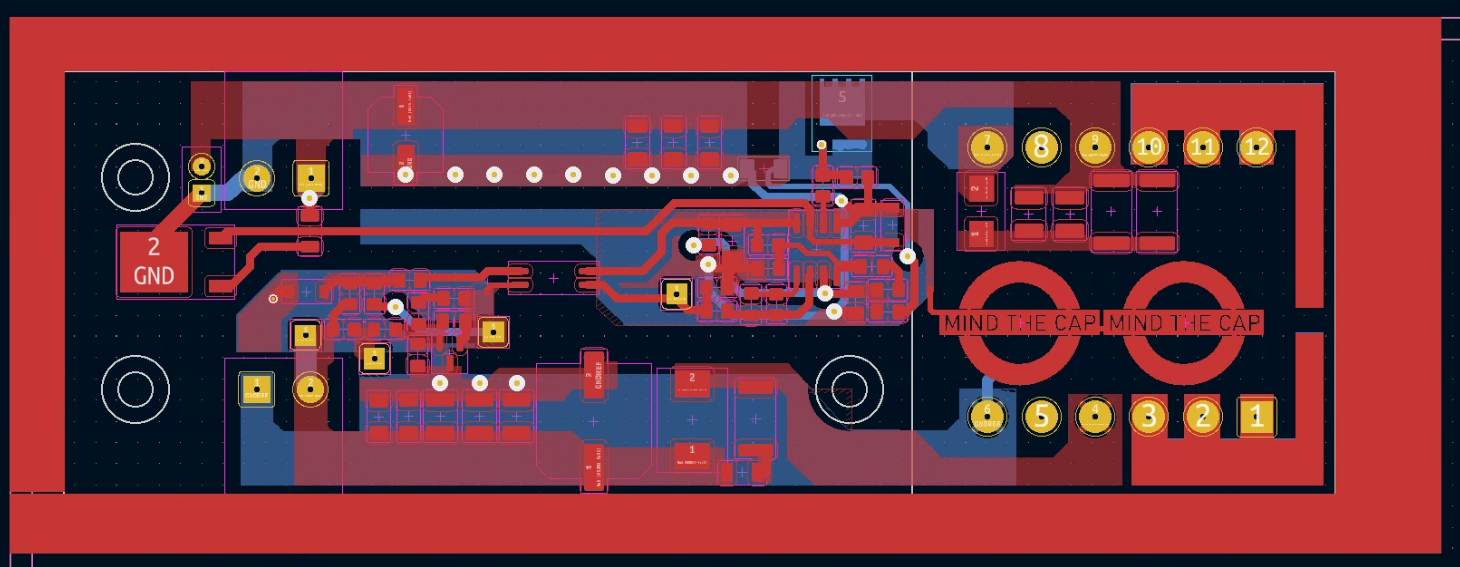
\includegraphics{img/pcb.png}}%
        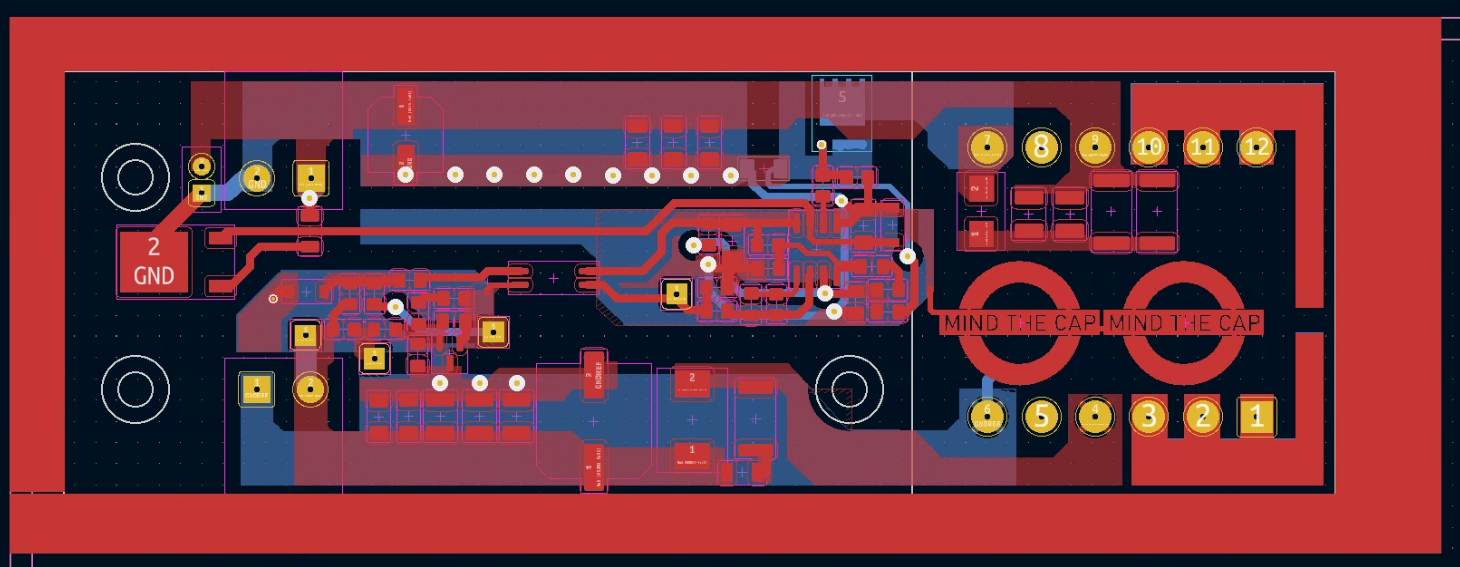
\includegraphics[clip,trim={.01\wd0} {.1\ht0} {.06\wd0} {.1\ht0},scale = 0.4]{img/pcb.png}
        \caption{PCB design with logo as the stitching capacitor.}
        \label{fig:tr_1}
    \end{figure}


Besides all these requirements, we wanted our converter to be small-sized and aesthetic. Also, we wanted to ease the production with adjusting proper spacing and positioning of the components and copper tracks. We designed our PCB by considering all of these requirements using KiCAD environment. \\

    \begin{figure}[H]
        \centering
        \sbox0{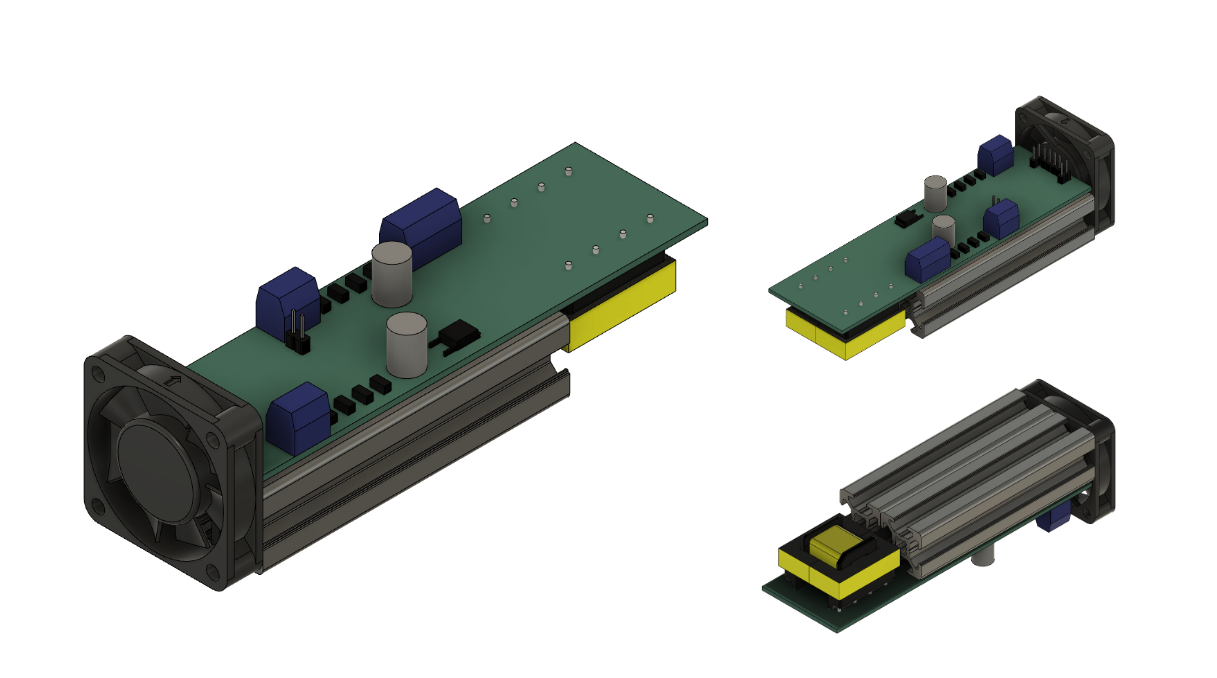
\includegraphics{img/mech.png}}%
        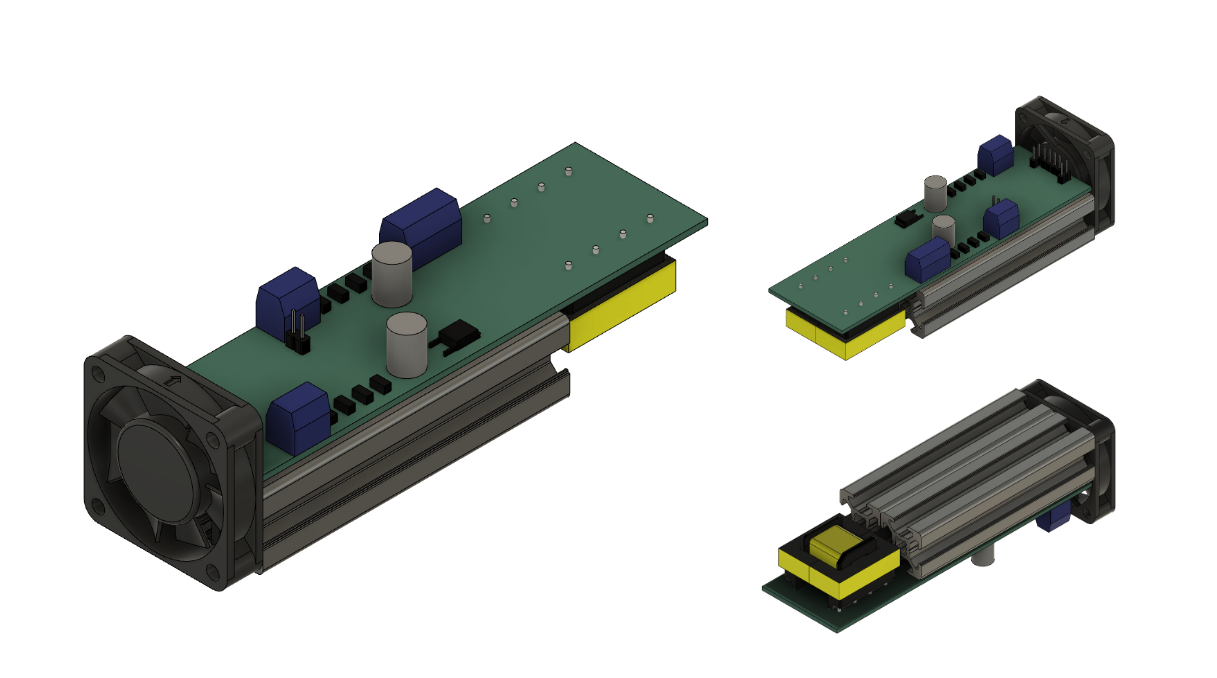
\includegraphics[clip,trim={.01\wd0} {.01\ht0} {.01\wd0} {.01\ht0},scale = 0.4]{img/mech.png}
        \caption{Initial thoughts on the mechanical and thermal aspects of the design.}
        \label{fig:tr_1}
    \end{figure}

An aluminum profile is used as a solid mechanical frame upon which the PCB will be constructed. This profile is also used as an heatsink to cool down the MOSFET in the circuit. Appropriate connectors are found for input and output connections. A place and a connector for a cooling fan is also placed for optional use. Finally, a plexiglass case is designed and produced for the converter. The photograph of the produced converter is given in Figure \ref{fig:produced_converter}. Size of the converter with the case is 50mm x 50mm x 140mm. \\

    \begin{figure}[H]
        \centering
        \sbox0{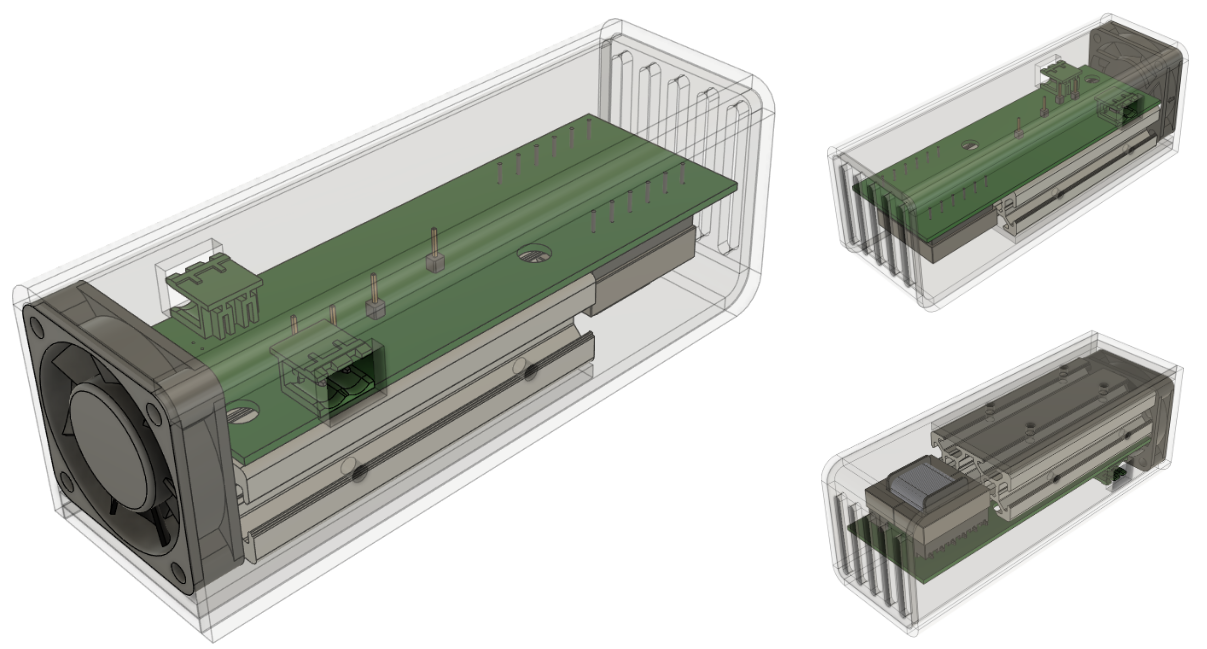
\includegraphics{img/final.png}}%
        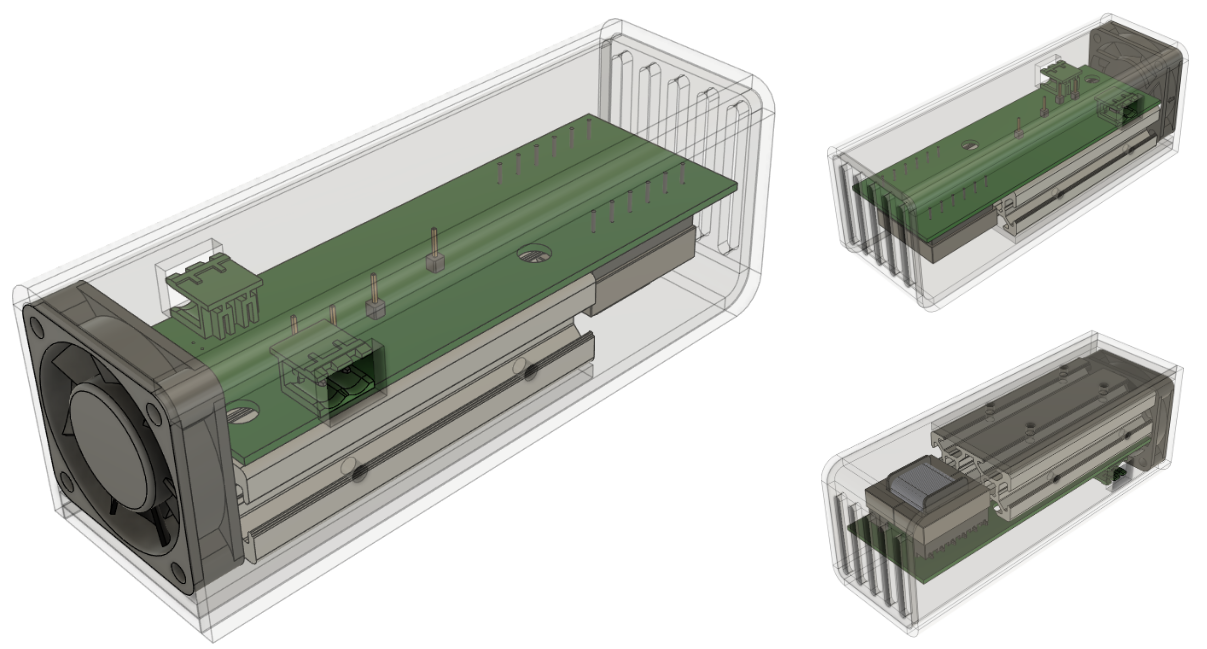
\includegraphics[clip,trim={.01\wd0} {.01\ht0} {.01\wd0} {.01\ht0},scale = 0.4]{img/final.png}
        \caption{Final 3D design and the acyrilic case.}
        \label{fig:tr_1}
    \end{figure}

\begin{figure}[H]
    \centering
    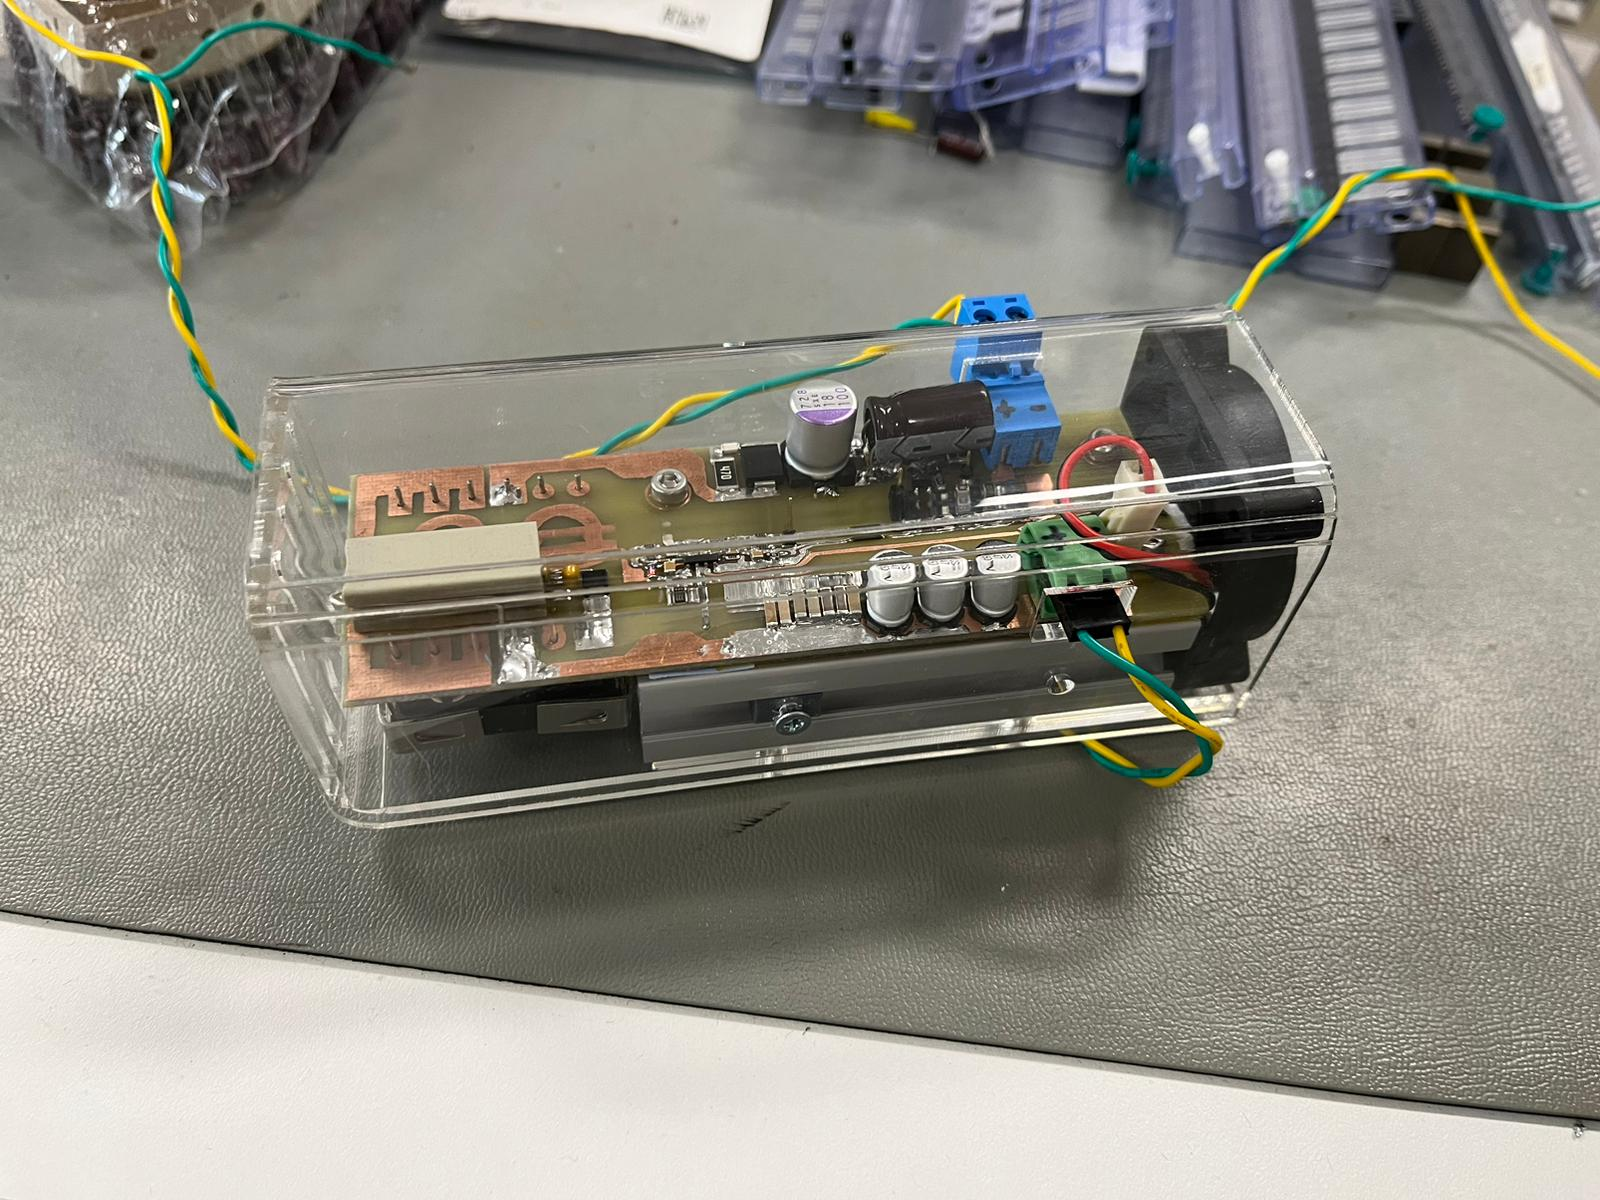
\includegraphics[scale=0.3]{img/sirin_mi_sirin_converter.jpeg}
    \caption{The 48V-48W flyback converter designed and produced by Mind the Cap}
    \label{fig:produced_converter}
\end{figure}

 \section{Experiments and Performance}
    Here we present the experimental data obtained during development and final demo.

    \begin{figure}[H]
        \centering
        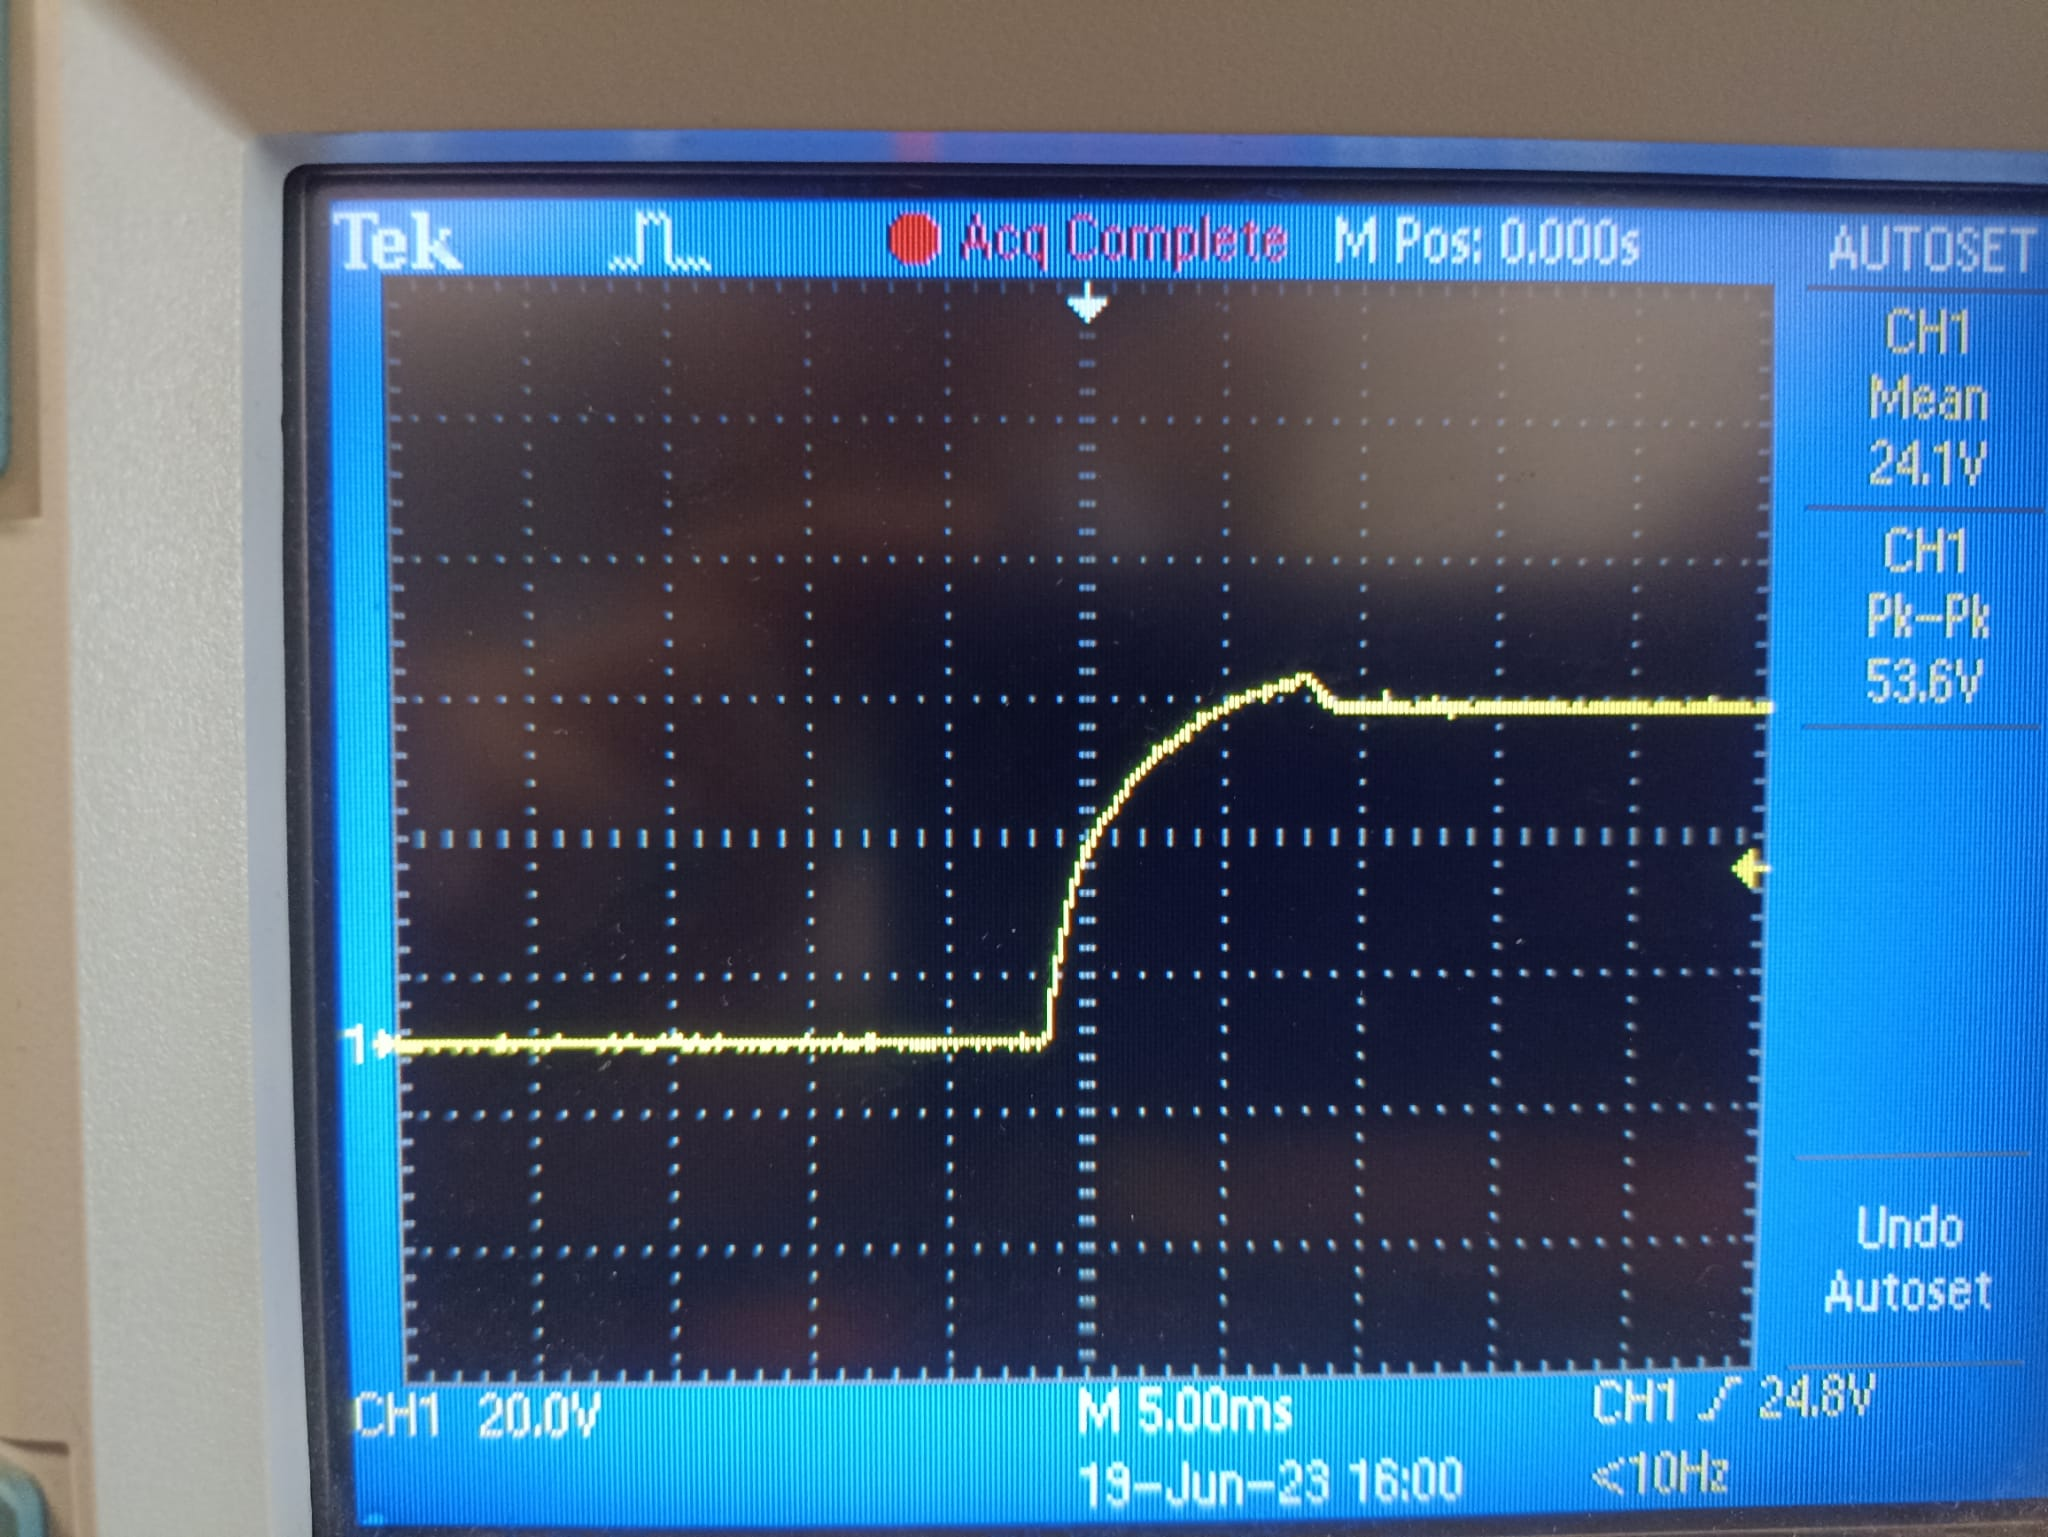
\includegraphics[width = \textwidth]{img/step_resp.jpeg}
        \caption{Step response to input voltage at half load}
        \label{fig:step-respo}
    \end{figure}

    Figure \ref{fig:step-respo} is the step response of the system to input voltage at half rated load. An overshoot is observed, which is likely caused by the lack of pole placement capacitor in the optocoupler network that adjusts the phase margin. The overshoot is about 5.6V corresponding to $11\%$ of the steady state voltage. This ratio indicates that the phase margin is less than $45^\circ$ under second order assumption. The figure also shows that the settling time is around 10ms.

    \begin{figure}[H]
        \centering
        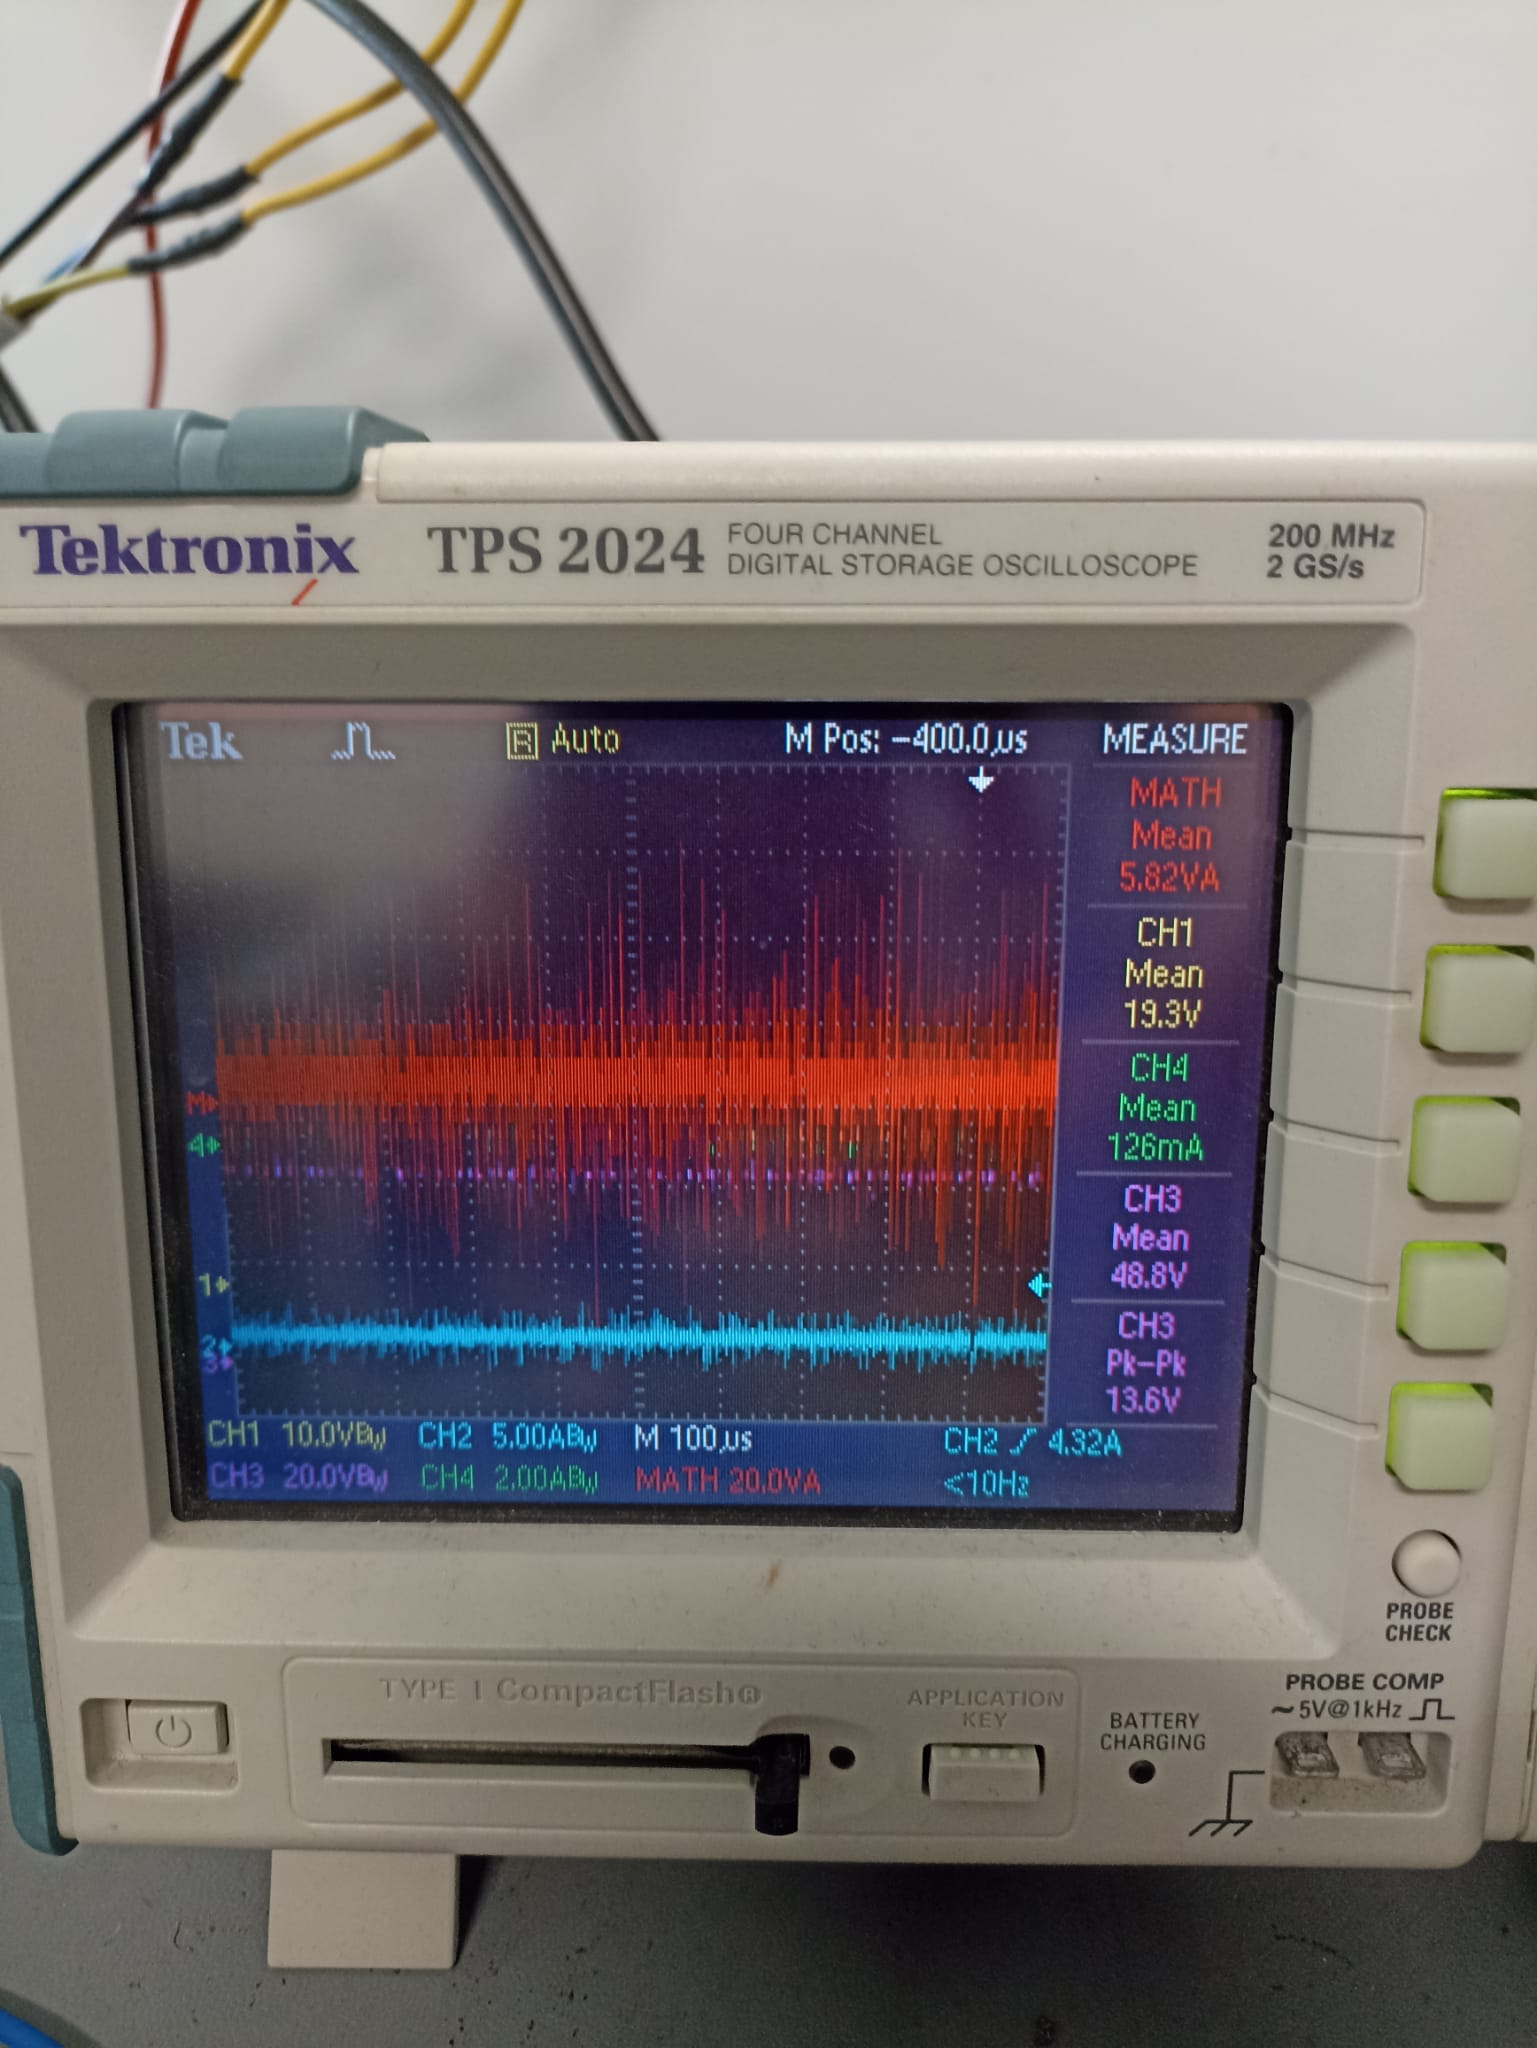
\includegraphics[width = \textwidth]{img/in1810perload.jpeg}
        \caption{Measurements at 18V input and $10\%$ load}
        \label{fig:meas-1}
    \end{figure}

    In Figure \ref{fig:meas-1} we see the measurements at $10\%$ load. At this stage, output was 48.488V.

    \begin{figure}[H]
        \centering
        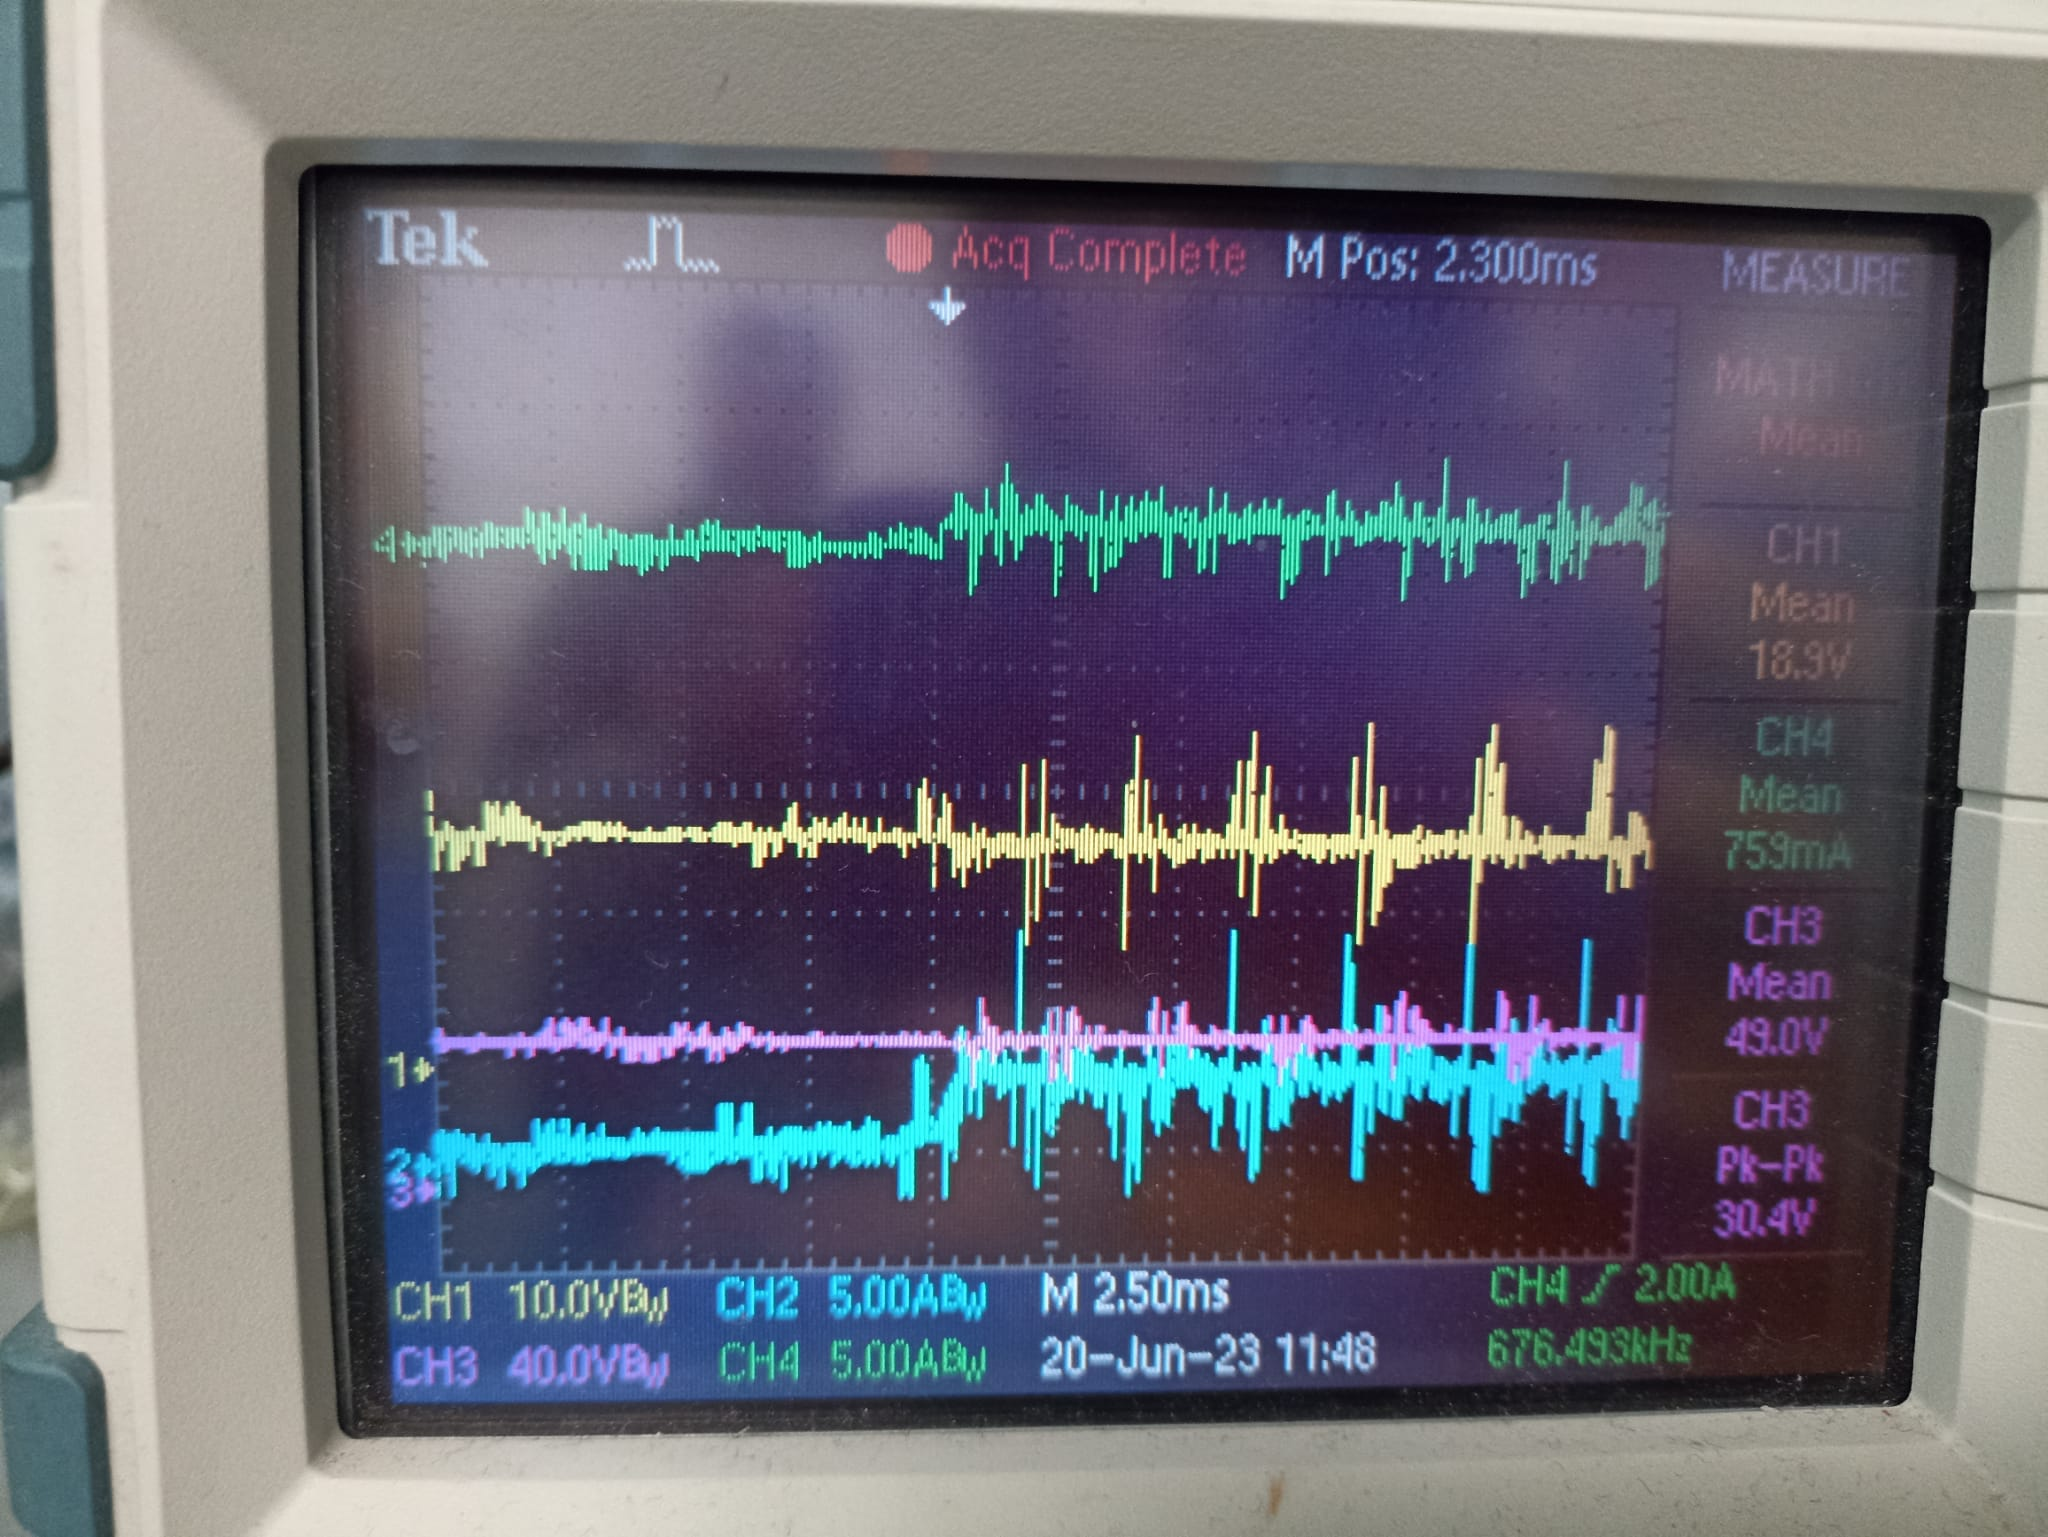
\includegraphics[width = \textwidth]{img/meas-load-change-to-76.jpeg}
        \caption{Measurements during load change to full load at 18V input}
        \label{fig:load-respo-76}
    \end{figure}
    
    In Figure \ref{fig:load-respo-76} we see the measurements during change to full load at 18V input.

    \begin{figure}[H]
        \centering
        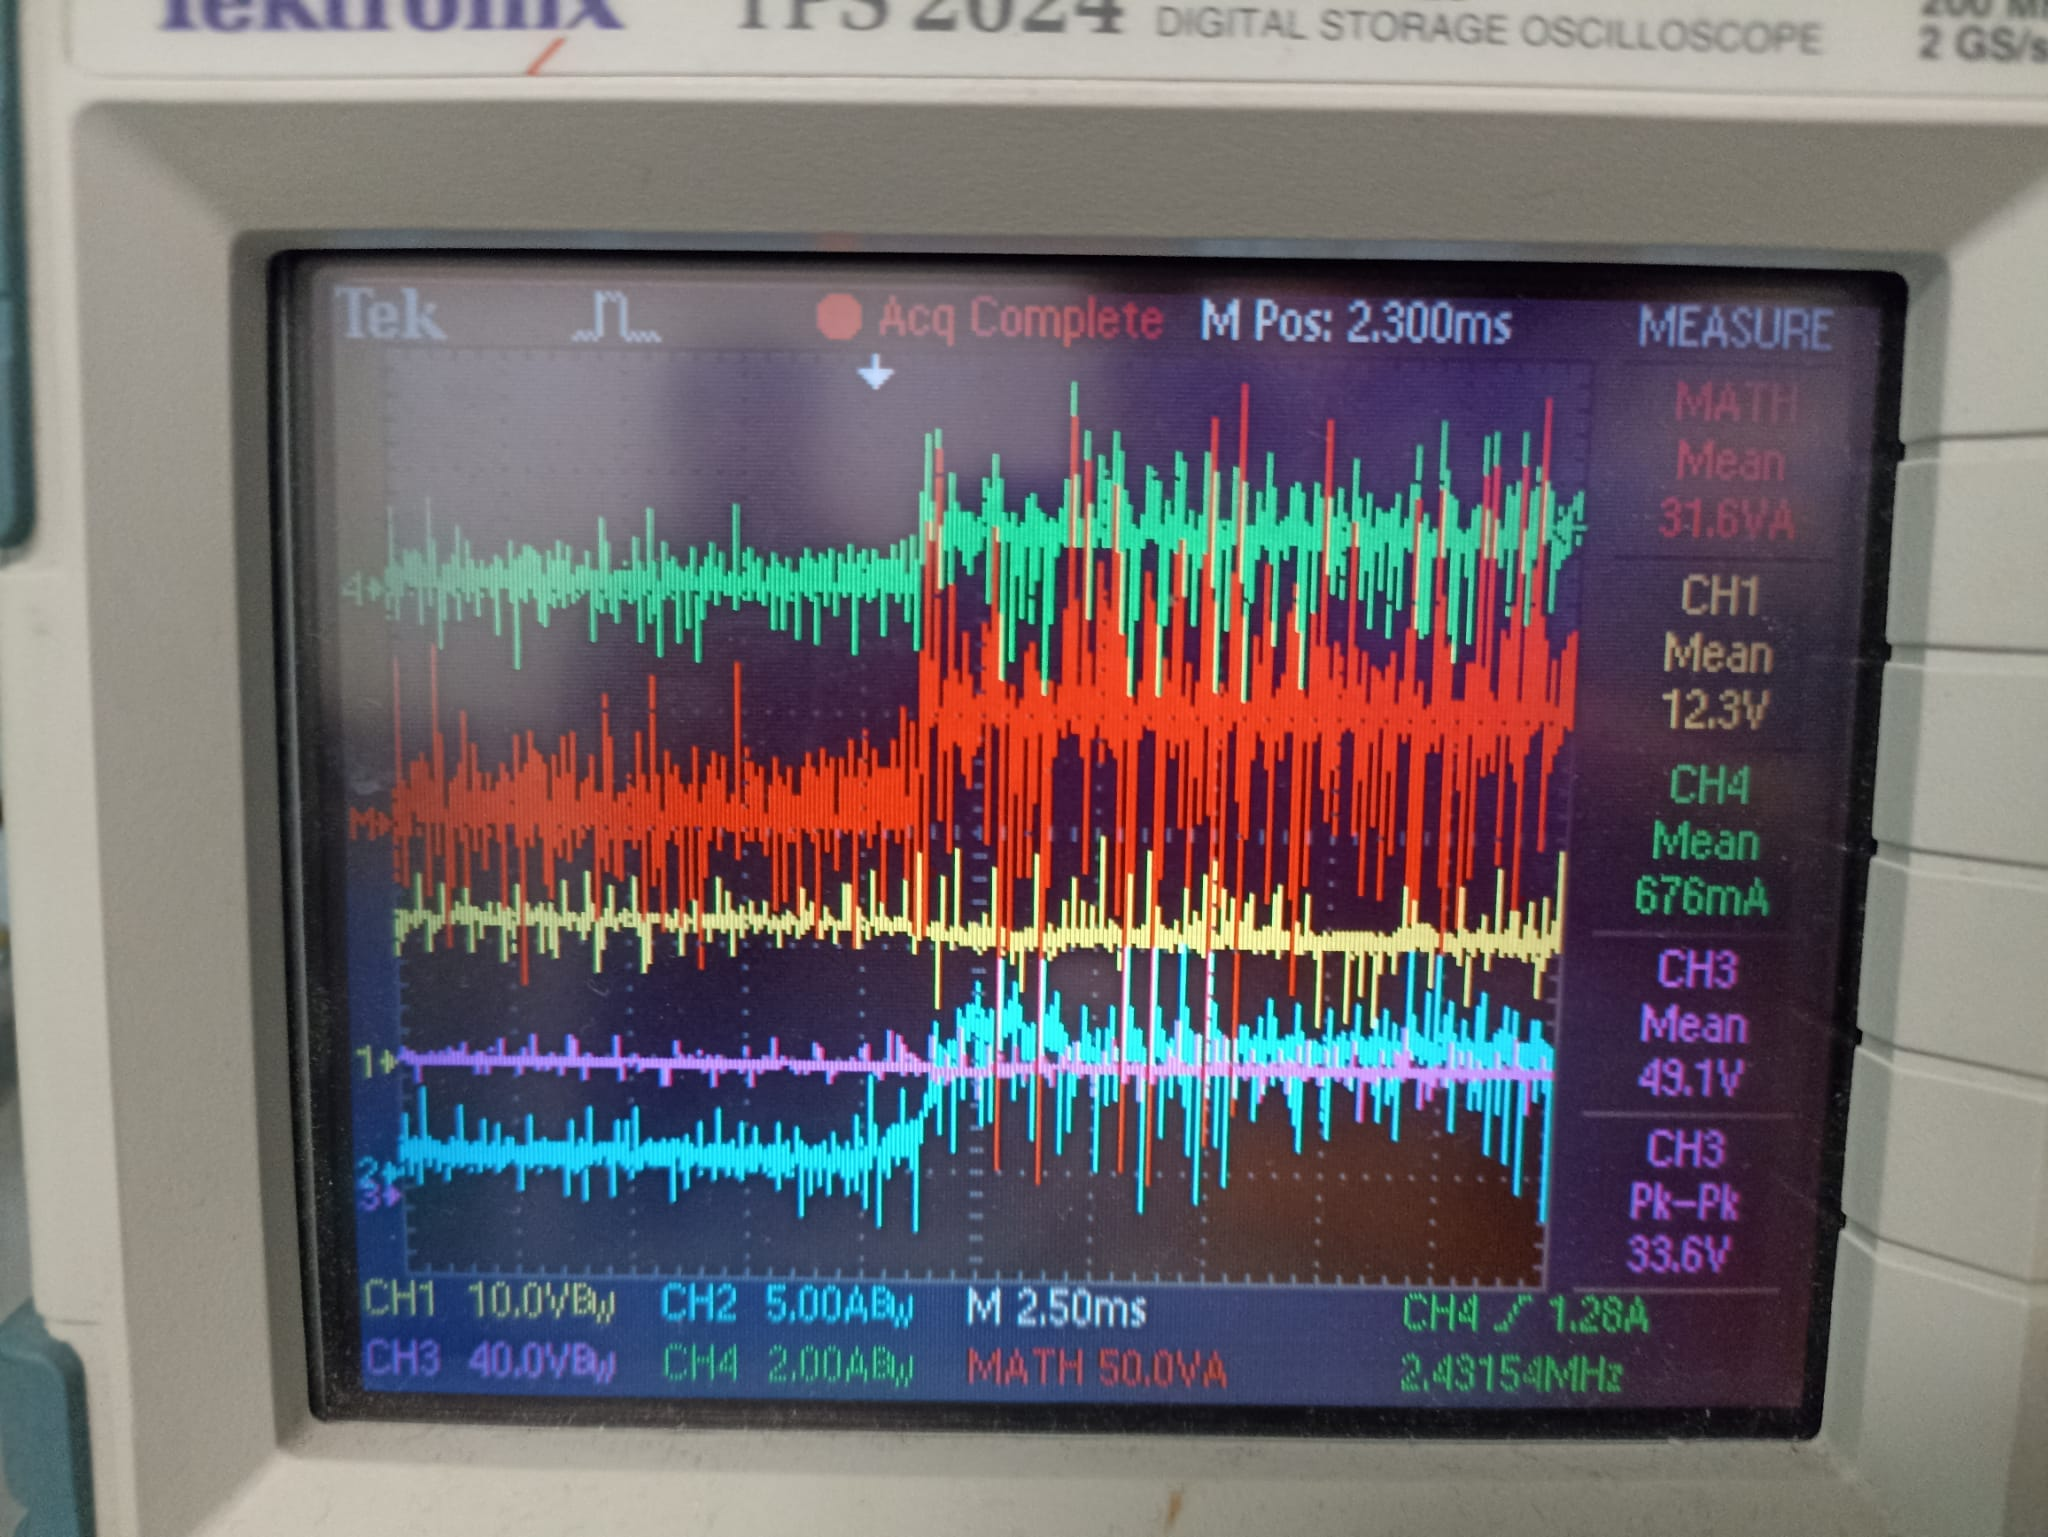
\includegraphics[width = \textwidth]{img/in12loachange.jpeg}
        \caption{Response to load change to full load at 12V input}
        \label{fig:load-respo-12}
    \end{figure}

    Figure \ref{fig:load-respo-12} is the response to load change at 12V. \\

    The efficiency is calculated at full load for 12V and 18V as 69\% and 74\%, respectively. Overall, except for the low efficiency (which is discussed to be expected for this flyback topology with this switching frequency and input-output voltage ranges) the control and regulation performance of the converter is satisfactory.
    
\section{Discussions  \& Conclusions}
In this report, the design process of a 48V-48W flyback converter is discussed extensively. It is observed that the control performance is robust during transients such as sudden load changes, and output voltage is consistently 48V, with a ripple less than 2\%. Snubber circuits are necessary for both primary and secondary sides to protect switching elements during turn-off moments of the switch, due to leakage inductance. However, the losses in the snubber circuit reduced the efficiency significantly. Hence, from an efficiency standpoint, it is observed that another topology such as two switch flyback would be more appropriate since it reduces the effects of the switching off the leakage inductance current and reduces the voltage stresses on the elements. Note that if one uses a lower switching frequency such as 50kHz, the subber losses will be reduced as well as other losses in the circuit, increasing the efficiency. In conclusion, flyback converter topology is still a simple and convinient topology with its simple control and low component count, making it a viable solution for isolated DC-DC converter applications.


\lstset{language=Matlab,%
    %basicstyle=\color{red},
    breaklines=true,%
    morekeywords={matlab2tikz},
    keywordstyle=\color{blue},%
    morekeywords=[2]{1}, keywordstyle=[2]{\color{black}},
    identifierstyle=\color{black},%
    stringstyle=\color{mylilas},
    commentstyle=\color{mygreen},%
    showstringspaces=false,%without this there will be a symbol in the places where there is a space
    numbers=left,%
    numberstyle={\tiny \color{black}},% size of the numbers
    numbersep=9pt, % this defines how far the numbers are from the text
    emph=[1]{for,end,break},emphstyle=[1]\color{red}, %some words to emphasise
    %emph=[2]{word1,word2}, emphstyle=[2]{style},    
}




\begin{thebibliography}{00}
    \bibitem{core}https://www.ferroxcube.com/upload/media/product/file/Pr\_ds/E30\_15\_7.pdf
    \bibitem{ic} https://ozdisan.com/entegre-devreler-ics/guc-entegreleri/dc-dc-voltaj-kontrolorleri/UC3843AN/732711
    \bibitem{mos} https://ozdisan.com/Product/Detail/594986/CSD19534Q5A
    \bibitem{diode} https://www.digikey.com/en/products/detail/diodes-incorporated/PDS3200-13/697102 
    \bibitem{cap} https://www.digikey.com/en/products/detail/samsung-electro-mechanics/CL31B225KCHSNNE/3888796
    \bibitem{clamp} https://www.digikey.com/en/products/detail/epcos-tdk-electronics/B66232A2010X000/3915550
    \bibitem{dcm} https://www.icbanq.com/icbank\_data/online\_seminar\_image/Flyback\_CCMVsDCM\_Rev1p2.pdf
    \bibitem{caps}
    https://www.ti.com/lit/an/slta055/slta055.pdf
\end{thebibliography}

\end{document}
